\documentclass[msc, classic, a4paper]{ufbathesis}
\usepackage[utf8]{inputenc}
\usepackage[brazil]{babel}
\usepackage{fancyvrb}
\usepackage[alf]{abntex2cite}
\usepackage{graphicx}
\usepackage{multicol}
\usepackage{enumitem}
\usepackage{float}
\usepackage{rotating}
\usepackage{tipa}
\usepackage{textcomp}
\usepackage{multirow}
\DeclareGraphicsExtensions{.pdf}

\defenseyear{2016}
\date{08 de Julho de 2016}
\adviser[f]{Profa. Dra. Christina von Flach G. Chavez}
\coadviser{Prof. Dr. Paulo Roberto Miranda Meirelles}

\title{
  Um estudo sobre a complexidade estrutural e o custo de mudança das
  ferramentas de análise estática de código-fonte
}

\author{Joenio Marques da Costa\\
  {\small joenio@joenio.me}
}

\begin{document}

\frontpage
\frontmatter
\presentationpage

\resumo

(pendente)
%Análise estática de código-fonte é um tema em constante evolução, ferramentas
%deste domínio continuam a ser desenvolvidas tanto na academia quanto na
%indústria, compreender os aspectos que refletem na manutenabilidade destas
%ferramentas é uma atividade primordial do ponto de vista dos desenvolvedores
%destas ferramentas. Neste sentido uma das abordagens é a observação dos valores
%de métricas de código-fonte, de forma a jogar luz sobre aspectos arquiteturais
%importantes que justifiquem ou denunciem problemas em sua qualidade interna.
%Assim utilizamos abordagens encontradas na literatura especializada sobre
%métricas de código-fonte para observação da complexidade estrutural e custo de
%mudança das ferramentas deste domínio de aplicação.

\begin{keywords}

  complexidade estrutural, custo de mudança, ferramentas de análise estática, engenharia de software.

\end{keywords}

\tableofcontents
\listoffigures
\listoftables

\mainmatter

%------------------------------------------%

%%

%%   * amadurecer as hipoteses, usar apenas paulo percentis, nao lanza, partir de chance cost
%%     enfatizar em change cost, deixar claro contribuicao, deixar claro contexto e problema
%%     questao de pesquisa nao deve citar thresholds, usar caracterizacao para separar entre
%%     linguagens e escolher um gold para cada e fazer estudo longitudinal, comparar longitudinalmente
%%     usando a numero de mudanças, num release com muitas mudanças teve aumento ou reducao no
%%     custo de mudança e na complexidade estrutural? 
%%   
%%   Piccinini and Gregory (2013) studied the nature of complexity in project and programs (set of related projects)
%%   through a systematic literature review. B
%%   
%%   lamantia2008: Our results
%%   provide positive evidence that DSM and DRT can
%%   inform important aspects of large-scale software
%%   structure and evolution, having the potential to guide
%%   software architecture design activities.
%%   
%%   Designers have long recognized the value of
%%   modularity. Constantine’s low-coupling, high-cohesion
%%   principle has been well known since the 1970’s [17].
%%   Parnas’s information hiding criterion [12] has
%%   remained influential for decades. Designers are
%%   educated to seek modular architectures to better
%%   accommodate expected changes and to enable parallel
%%   development.
%%   
%%   Baldwin and Clark’s theory, which is based on
%%   Steward’s [17] design structure matrix (DSM)
%%   modeling approach (described below), argues that
%%   design rules can be used to resolve interdependencies
%%   and create modular architectures by specifying the
%%   interface between modules. Sullivan et al. [18] applied
%%   this approach to Parnas’s [13] small but canonical Key
%%   Word in Context (KWIC) design example. They show
%%   that DSM models and design rule theory can precisely
%%   capture Parnas’s information hiding criterion.
%%   
%%   24.pdf: Complexity measures are very useful in identifying complex program units. Numerous
%%   research studies investigated the relationship between program complexity and maintain-
%%   ability [27]. These studies have found that complex systems requires a lot of e ort in
%%   maintaining them. Simplifying your components usually leads to reducing the maintenance
%%   cost. Large values for CC hinder the software evolution since they make the program both di
%%   cult to change and to understand [23].
%%   
%%   Software complexity is considered a major player in the software engineering research and
%%   practice [7, 6], and it is the result of the design decision, algorithm choices, and the
%%   implementation details, also it can be used to predict several quality characteristics; such as
%%   maintainability [18, 6]. For example, high complex modules have been found to be most
%%   prone to faults [30]. Therefore, monitoring and controlling of a given software is very
%%   essential to the its project success.

%% Segundo definição PMBOK\cite{Pmbok2013} {\it threshold} é traduzido como ``Limite'':
%% 
%% \begin{quote}
%% Um valor de custo, de tempo, de qualidade,
%% técnico ou de recurso usado como parâmetro e
%% que pode ser incluído nas especificações do
%% produto. Ultrapassar o limite deve provocar
%% alguma ação, como a geração de um relatório de
%% exceções.
%% \end{quote}
%% 
%% Lorenz and Kidd propose threshold
%% values for several object-oriented metrics for C++ and
%% Smalltalk based on their experience with selected C++
%% and Smalltalk projects [11]. - Object-oriented software metrics: a practical guide
%% 
%% \cite{El2001}
%% 
%% Bowen (Bowen, 1984) proposed component size thresholds between 23-76 source
%% statements based on his own analysis. After a lengthy critique of size
%% thresholds, Dunn and Ullman (Dunn and Ullman, 1979) suggest two pages of
%% source code listing as an indicator of an overly large component. Woodfield et
%% al. (1981) suggest a maximum threshold of 70 LOC.
%% 
%% For example, Lorenz and
%% Kidd (Lorenz and Kidd, 1994), based on their experiences with Smalltalk and
%% C++ projects, recommended an inheritance nesting level threshold of 6,
%% indicating that inheritance up to a certain point is not detrimental.
%% 
%% A recent series of studies led by the author investigated thresholds for object-
%% oriented metrics (Benlarbi et al., 2000; El-Emam, Benlarbi, Goel, Melo et al.,
%% 2000; Glasberg et al., 2000). The first study demonstrated that an absence of
%% size thresholds for object-oriented classes (El-Emam, Benlarbi, Goel, Melo et
%% al., 2000). The remaining two studies demonstrated that an absence of threshold
%% effects for a subset of the metrics described earlier (Benlarbi et al., 2000;
%% Glasberg et al., 2000). The results are consistent across all of the three studies:
%% there are no thresholds for contemporary object-oriented metrics, including class
%% size.
%% 
%% \cite{Shatnawi2006}
%% There were enormous empirical studies that validated
%% Object-Oriented (OO) metrics as predictors of software
%% quality [1][4][6]. However, there is still a dearth of studies
%% that identified the threshold values of OO metrics.
%% 
%% Bender pointed out that these
%% thresholds should only be considered as valid threshold
%% values if the prediction model’s assumption, i.e. a
%% constant risk below the threshold, is plausible [2]. Bender
%% proposed a quantitative method for identifying threshold
%% values from a logistic regression curve. In this paper, we
%% identify the threshold values of CK [5] metrics using
%% Bender methodology [2].
%% Metrics
%%     VARL1  VARL2
%% CBO 24     10
%% RFC 161    55
%% WMC 102    33
%% 
%% \cite{Sant2008}
%% The problem is far from being new and it
%% characterizes intrinsically any metrics-based approach. In most of the cases setting
%% the threshold values is a highly empirical process and it is guided by similar past
%% experiences and by hints from metrics’ authors (Lorenz & Kidd, 1994).
%% 
%% \cite{Clauset2009} faz um estudo detalhado da power-law em dados empiricos, n eh sobre metricas de software, teorico sobre estatistica
%% 
%% \cite{Ferreira2009}
%% evidenciam valores
%% que podem ser tomados como referência para as medidas das
%% métricas.
%% 
%% ainda está em aberto a definição
%% dos valores desejáveis para essas métricas, o que restringe
%% o uso efetivo de métricas na produção de software.
%% 
%% V ALORES REFER ÊNCIA PARA M ÉTRICAS OO
%% Fator Nı́vel Métrica Valor Referência
%% 
%% Conectividade
%% Sistema: COF Bom: até 0,02 - Regular: entre 0,02 e 0,14 - Ruim: maior ou igual a 0,14
%% Classe: # conexões aferentes Bom: 1 - Regular: entre 1 e 20 - Ruim: maior ou igual a 20
%% 
%% Ocultação de Informação
%% Classe: # atributos públicos Bom: 0 - Regular: entre 0 e 8 - Ruim: maior ou igual a 8
%% 
%% Tamanho da Interface
%% Classe: # métodos públicos Bom: 0 a 10 - Regular: entre 10 e 40 - Ruim: maior ou igual a 40
%% 
%% Herança
%% Classe: DIT (profundidade na árvore de herança) Valor tı́pico: 2
%% 
%% Coesão Interna
%% Classe: LCOM (ausência de coesão) Bom : 0 - Regular: entre 0 e 20 - Ruim: maior ou igual a 20
%% 
%% \cite{Shatnawi2010}
%% The focus of the study is to identify threshold values of software metrics using receiver
%% operating characteristic curves.
%% 
%% This method has not been used before to identify OO metric threshold values.
%% 
%% very
%% few have identified threshold values of metrics and suggested guidelines on how to interpret and
%% apply these values.
%% 
%% Table X. Candidate threshold values.
%% Metrics Threshold values
%% RFC 44
%% CTM 33
%% CBO 13
%% WMC 24
%% NOO 9
%% 
%% Although we analyzed only one system in our study, we believe that the research results can
%% be generalized to the OO systems that are similar to Eclipse—an industrial-strength system that is
%% continuously evolving with thousands of classes.
%% 
%% \cite{Herbold2011}
%% Table 2 Threshold values for the metrics to measure the maintainability
%% 
%% WMC Java 100 Benlarbi et al. (2000)
%% CBO Java 5 Benlarbi et al. (2000)
%% RFC Java 100 Benlarbi et al. (2000)
%% NORM Java 3 Lorenz and Kidd (1994)
%% LOC Java 500 Adapted from Copeland (2005)
%% NOM Java 20 Adapted from Copeland (2005)
%% NSM Java 4 Lorenz and Kidd (1994)
%% 
%% \cite{Ferreira2012}
%% define limites por dominio, por tipo de software e por tamanho
%% 
%% \cite{Zhang2013}
%% o contexto influencia a distribuicao das metricas, ou seja, linguagem
%% de programacao afeta, o dominio, etc...
%% 
%% Contexts of software systems are considered in Ferreira et
%% al. [14]’s work. They propose to identify thresholds of six
%% object-oriented software metrics using three context factors:
%% application domain, software types and system size (in terms
%% of the number of classes).
%% 
%% Este autor => application domain, pro-
%% gramming language, and the number of changes,
%% 
%% Open source software systems are characterized by
%% Capiluppi et al. [22] using 12 context factors: age, appli-
%% cation domain, programming language, size (in terms of
%% physical occupation), the number of developers, the number
%% of users, modularity level, documentation level, popularity,
%% status, success of project, and vitality.
%% 
%% Number of Changes (NC): describes the total number of
%% commits made to a software system. It might be more difficult
%% to maintain heavily-modified software systems than lightly-
%% modified ones.
%% 
%% Este autor => The most influential factors are application
%% domain, programming language, and the number of changes.
%% 
%% \cite{Oliveira2015}
%% Our preliminary results indicate
%% that good quality applications—as cited by experts—respect
%% metric thresholds. In contrast, we observed that noncompliant
%% applications are not largely viewed as requiring more effort to
%% maintain than other applications.
%% 
%% To address the challenge of identifying thresholds that have to
%% In this section we summarize the proposed technique for
%% be followed by many but not all methods, classes or components extracting relative thresholds from a Corpus, a benchmark of
%% we have introduced in previous work the notion of a relative software applications [6], [7]. This technique derives thresholds
%% threshold [6], [7]. Relative thresholds are represented by pairs represented by pairs [p, k], such that p% of the classes in an
%% (p, k) such that p% of the classes in an application should have application should have M ≤ k. Therefore, a relative threshold
%% M ≤ k, where M is a given source code metric and p is the tolerates (100 − p)% of classes with M > k. As an example,
%% minimal percentage of classes in each application that should we can derive a relative threshold as follows: at least 75% of
%% respect the upper limit k.
%% 
%% For each application, we evaluate their percentage of classes
%% respecting the k-value of the proposed relative threshold. The
%% results are summarized in Table IV. For instance, the relative
%% threshold for NOA is (75, 5) and the table shows that 100%
%% of the classes of PetitParser have five attributes or less.
%% 
%% introduz o conceito de threshold relatives (bom p eu usar igual)
%% 
%% \cite{Gil2016}
%% code
%% metrics such as lines of code are extremely context dependent and their distri-
%% bution differs from project to project.
%% 
%% metric values are so sensitive
%% to context, that their measurement in one project offers little prediction regarding
%% their measurement in another project.
%% 
%% % ---
%% 
%% terceiro:
%% 
%% As proposições da teoria proposta por terceiro:
%% 
%% P7 A complexidade estrutural influencia positivamente o esforço necessário para a ati-
%% vidade de compreensão de software, um aumento
%% na complexidade do software implica em um aumento no esforço necessário para
%% que desenvolvedores consigam compreender a arquitetura do software.
%% 
%% P8 O esforço necessário para compreensão de um sistema de software influencia positi-
%% vamente o esforço necessário para realizar atividades de manutenção, um aumento
%% no esforço para compreensão acarreta um aumento no esforço necessário para rea-
%% lizar atividades de manutenção.
%% 
%% P9 O esforço necessário para atividades de manutenção influencia positivamente os cus-
%% tos de projetos de software.
%% Explicação: Se os desenvolvedores têm maior dificuldade para compreender e mo-
%% dificar sistemas de software, os custos do projeto de manutenção de tal sistema
%% tendem a subir. Os desenvolvedores precisam de mais tempo para realizar as mu-
%% danças, o que, por consequência, faz com que o projeto consiga alcançar menos
%% resultados com os recursos disponı́veis.
%% 
%% P7 é considerada como proposição válida com base na literatura existente (Darcy et
%% al., 2005; Midha, 2008) (capı́tulo 3), e é considerada como justificativa para os estudos
%% realizados.
%% P8 e P9, propondo que o esforço de compreensão influencia positivamente no esforço
%% de manutenção e que este influencia nos custos do projeto, são consideradas axiomas.
%% Isto é, elas são assumidas como verdadeiros dentro do nosso domı́nio de análise, e servem
%% de ponto de partida para inferir outros fatos na nossa teoria.
%% 
%% ---
%% 
%% Outra possibilidade de trabalho futuro é explorar diferentes aspectos da complexi-
%% dade estrutural. A métrica utilizada neste trabalho para complexidade estrutural de um
%% projeto representa a complexidade estrutural média entre os seus módulos. O uso apenas
%% da média não leva em consideração a distribuição da complexidade entre os módulos, ou
%% seja, a variância. Dois projetos, ou dois momentos no histórico de um mesmo projeto, que
%% possuam a mesma complexidade estrutural média mas variâncias diferentes, podem apre-
%% sentar desafios diferentes à atividade de manutenção. Por exemplo, uma baixa variância
%% implica que a complexidade é distribuı́da de forma mais uniforme entre os módulos, o que
%% pode indicar um problema estrutural grave cuja resolução demandaria bastante esforço.
%% Já uma variância alta pode indicar que o excesso de complexidade estrutural está loca-
%% lizado num subconjunto do módulos, o que pode eventualmente ser solucionado através
%% de um esforço localizado de reengenharia. Este tipo de análise pode ajudar a identificar
%% problemas de design em sistemas de software.

\xchapter{Introdução}{}

"Ocorrências não reprodutíveis não têm significado para a ciência" \cite{popper2004logica}.

\section{Motivação}

Em 2010, ... contar o cenário que envolve Analizo.

Eu, como engenheiro de software pesquisador e parte do ecossistema do software
acadêmico de análise estática Analizo estou interessado em saber como melhor
investir recursos no ecossistema do projeto Analizo com o objetivo de fazê-lo
mais útil e acessível para todo o campo de pesquisa, uma vez que percebo que os
projetos de software do meu campo sofrem da existência de muitos projetos, com
poucos usuários, com ciclos de vida curtos, que terminam em paralelo ao
financiamento inicial, comunidades desconectadas e paralelas,
incompatibilidades entre projetos, e tentativas aparentemente não coordenadas
de ``reiniciar'' tudo ({\it re-boots}).

Mas antes de saber como atingir este objetivo é necessário compreender como
este problema ocorre e se ele realmente acontece no ecossistema de software
acadêmico de análise estática.

% é interessante realmente apresentar o Analizo como um case de sucesso

%software acadêmicos sofrem de {\it ``dysfunctional chaotic churn''}.
% O ecossistema de software acadêmico sofre de um fenômeno chamado de
% desordem caótica disfuncional ({\it ``dysfunctional chaotic churn''}).

\section{Apresentação}

A Ciência moderna depende de software. Novos softwares são constantemente
criados e desenvolvidos durante pesquisas científicas, seja pelo próprio pesquisador,
seja por colaboradores. 
Estes softwares resolvem problemas comuns de pelo menos metade dos cientistas 
de todas as áreas da Ciência, em atividades de coleta ou análise, 
e em outras atividades de pesquisa.

Estes softwares variam em tamanho e finalidade: alguns são simples
scripts para automatizar tarefas repetitivas, enquanto outros são utilizados para
coleta, análise ou transformação de dados. Alguns softwares são projetos maduros e
carregam boa parte do conhecimento desenvolvido ao longo da própria pesquisa, e
costumam ter uma maior promoção por parte dos seus autores e um maior
reconhecimento por parte da comunidade científica.

O domínio e objetivo da pesquisa também implicam em particularidades do software: 
um software para coleta de dados numa pesquisa em engenharia de
software certamente terá características e requisitos distintos de um software
para o mesmo fim em outro domínio, por exemplo,  antropologia ou medicina.
Em um mesmo domínio, softwares para análise de dados podem variar
enormemente entre sí, dependendo do objetivo da pesquisa e das atividades realizadas.
\'{E} natural acreditar, portanto, que existe demanda suficiente para a
criação de softwares para os mais diversos campos de atuação e aplicação da
Ciência.

A criação destes softwares tem motivações variadas:  alguns cientistas publicam
seus softwares juntamente com dados e outros artefatos, outros fazem um esforço
adicional para documentar e incentivar o seu uso e adoção, alguns não
consideram seus softwares dignos de publicação, outros não dão visibilidade a
sua existência mesmo quando são publicados sob as melhores práticas da
engenharia de software.

Independente da finalidade, tamanho ou motivação, todo software tem o potencial
de voltar a ser útil em outros momentos ou lugares, para o autor original,
ou para pesquisadores enfrentando problemas semelhantes aos dos autores originais.
Não é difícil imaginar que o problema enfrentado por um pesquisador pode, em
algum momento, ser enfrentado por outros pesquisadores, criando assim uma ótima
oportunidade de colaboração entre pesquisas e pesquisadores, sendo o software
um excelente vetor de ajuda mútua em ambas as direções.

Apesar disso, cientistas tem percebido que os softwares desenvolvidos na
academia sofrem de {\it ``dysfunctional chaotic churn''}, ou seja, a existência
de muitos projetos, com poucos usuários, com ciclos de vida curtos, que
terminam em paralelo ao financiamento inicial, comunidades desconectadas e
paralelas, incompatibilidades entre projetos, e tentativas aparentemente não
coordenadas de ``reiniciar'' tudo ({\it re-boots}).

%Este cenário, além de desacelerar o progresso geral da ciência gerando
%retrabalho, faz surgir questionamentos sobre as conclusões dessas pesquisas,
%especialmente quando grande parte dos pesquisadores não sabem o quão confiável
%seus softwares são.

Este problema apesar de ser percebido por muitos cientistas carece de
evidências, neste trabalho investigamos como ele se manifesta em pesquisas da
engenharia de software, em especial, em publicações de análise estática, uma
área com uma longa e respeitável tradição em pesquisas sobre a criação de novas
ferramentas, métodos e algoritmos.

\section{Escopo}

O objetivo geral desta pesquisa é explorar como o {\it ``dysfunctional chaotic
churn''} se manifesta entre os projetos de software de análise estática,
respondendo as seguintes questões:

\begin{itemize}
  \item Projetos de software acadêmico de análise estática tem contribuidores além dos autores iniciais?
  \item Os projetos incentivam ativamente a contribuição?
  \item Os espaços dos projetos são abertos e transparentes?
  \item Os projetos fazem um pedido explícito e claro de reconhecimento?
\end{itemize}

Que tal perguntas assim?
\begin{itemize}

  \item Os projetos sustentáveis tem contribuidores além dos autores iniciais?
  \item Os projetos sustentáveis tem mais contribuidores?
  \item Os artigos de projetos sustentáveis são mais lidos, mais citados?
  \item Os autores de projetos sustentáveis tem mais publicações com o uso de software do que os autores?
  \item Os projetos são mais fáceis de manter?  de usar? 
\end{itemize}



Estas questões darão importantes indícios sobre a qualidade do software acadêmico de
análise estática desenvolvido na academia, especialmente sobre a capacidade de serem 
encontrados, compartilhados e co-desenvolvidos.

\section{Metodologia de trabalho}

(apresentar aqui um resumo do capítulo \ref{metodologia})

Objetivo específico: caracterizar software acad publicado quanto a ...
Objetivo específico: caracterizar o tipo de citação / menção d
  \item Os projetos tem contribuidores além dos autores iniciais?
  \item Os projetos incentivam ativamente a contribuição?
  \item Os espaços dos projetos são abertos e transparentes?
  \item Os projetos fazem um pedido explícito e claro de reconhecimento?

\section{Contribuições}

(pendente)

\section{Organização do texto}

(pendente)

%O capítulo \ref{fundamentacao} apresenta os fundamentos teóricos necessários
%para a compreensão deste trabalho.
%
%O capítulo \ref{metodologia} apresenta a estratégia de pesquisa adotada nos
%estudos.
%
%O capítulo \ref{sustentabilidade-tecnica} traz um estudo sobre a
%sustentabilidade técnica e a disponibilidade dos softwares acadêmicos de
%análise estática.
%
%O capítulo \ref{complexidade-ferramentas} descreve um estudo sobre a
%manutenabilidade dos softwares acadêmicos de análise estática.
%
%O capítulo \ref{conclusoes} apresenta as considerações finais e discute os
%resultados deste trabalho.

% A Retrospective Study of Academic Software Projects
% (estudo restropectivo parece um bom termo, uma busca rápida no google-scholar retornou muita coisa da área de saúde)



%------------------------------------------%

% A Preliminary Literature Review which indicates: 
% (i) that you have studied the work of the major authors in your research field 
% (ii) that you are familiar with the major themes relevant to that subject area 
% (iii) what further investigations you intend to pursue as part of this dissertation. 
% You should bear in mind that you are reviewing the literature in order to develop sharper, 
% more insightful and focused research questions about your topic. 
% Therefore, your literature review should lead to and justify your research objectives and questions.

% continuar a partir de:
% /home/joenio/src/bibliografia/Papers/Replication of Controlled Experiments in Empirical Software Engineering - A Survey.pdf

\xchapter{Fundamentação teórica}
{Este capítulo apresenta conceitos necessários para a compreensão do trabalho.}
\label{fundamentacao}

%\section{Software acadêmico}
%
%% Anúncio em destaque no ACM DL: Reproducibility of Results in the ACM Digital Library 
%% http://dl.acm.org/docs/reproducibility.cfm
%
%% ciencia aberta e desenvolvimento sustentavel
%% https://ocsdnet.org/open-and-collaborative-science-using-knowledge-as-a-pathway-to-sustainable-development/
%
%Segundo \citeonline{hettrick_2014_14809} software acadêmico ({\it research
%software}) é todo software usado para gerar, processar ou analisar resultados
%de pesquisas com intenção de ser publicados (seja num jornal, revista,
%conferência, monografia, livro ou tese). Software de pesquisa pode ser qualquer
%coisa entre poucas linhas escritas por você mesmo, até mesmo um software
%desenvolvido profissionalmente. Software que não gera, processa ou analisa
%resultados - como por exemplo um editor de textos, ou o uso de navegadores web
%- não são considerados softwares de pesquisa, segundo esta definição.
%
%%% Softwares acadêmicos são softwares desenvolvidos no decorrer de pesquisas
%%% científicas como parte de um estudo a ser publicado (seja num jornal, revista,
%%% conferência, monografia, livro ou tese), podem ser pequenos scripts contendo
%%% poucas linhas de código, protótipos, ou mesmo produtos de software completos
%%% que demonstram ou refletem os resultados de uma pesquisa, costumam ser
%%% utilizados para gerar, processar ou analisar resultados, mas podem ser para
%%% qualquer outro fim, basta que seja um dos artefatos gerado na pesquisa, será
%%% considerado software acadêmico.
%%% 
%%% Tais softwares podem ser encontrados na literatura pelo nome de {\it research
%%% tool} \cite{Portillo12}, {\it research-originated software} \cite{Kon2011},
%%% %{\it research software} \cite{hettrick_2014_14809} ou
%%% {\it academic software} \cite{allen2017engineering}, e costumam ser citados
%%% pelos seus autores como uma contribuição do estudo, seja principal ou
%%% secundária, alguns autores criam softwares acadêmicos como meio para atingir os
%%% resultados da pesquisa e não descrevem muito bem o software.
%%% 
%%% %, traduzido para software acadêmico para evitar o
%%% %termo {\it software de pesquisa}, a palavra {\it research} em português {\it
%%% %pesquisa} pode ser facilmente confundida com ferramentas ou sistemas de
%%% %pesquisa, como sites de pesquisa por exemplo,
%%% 
%%% % este artigo \cite{howison2016software} faz exatamento o mesmo estudo que estou fazendo!
%%% 
%%% Copiar e usar exatamente esta linha de pensamento e argumentos:
%%% Yet, the visibility of software in the scientific record is in
%%% question, leading to concerns, expressed in a series of
%%% National Science Foundation (NSF)- and National Institutes
%%% of Health–funded workshops, about the extent that scientists
%%% can understand and build upon existing scholarship (e.g.,
%%% Katz et al., 2014; Stewart, Almes, & Wheeler, 2010). In
%%% particular, the questionable visibility of software is linked to
%%% concerns that the software underlying science is of question-
%%% able quality. These quality concerns are not just technical,
%%% but extend to the appropriateness of software for wide
%%% sharing, and its ability to facilitate the codevelopment that
%%% would make efficient use of limited scholarly funding
%%% (Howison & Herbsleb, 2013; Katz et al., 2014).
%%% The link is two-fold: First, when software is not visible, it
%%% is often excluded from peer review; second, its lack of
%%% visibility, or the particular form of visibility, means that
%%% incentives to produce high-quality, widely shared, and code-
%%% veloped software may be lacking. A well-functioning system
%%% would assist not only the goals of understanding and trans-
%%% parency, but also the goals of aiding replication (Stodden
%%% et al., 2010), complementing the availability of publications
%%% such that “the second researcher will receive all the benefits
%%% of the first researcher’s hard work” (King, 1995, p. 445).
%%% The situation with software is broadly analogous (but not
%%% identical) to that of data in publications; indeed, all data are
%%% processed by software in some form (Borgman et al., 2012).
%%% Nonetheless, there are relevant differences. Accordingly, our
%%% inquiry into the visibility of software in scholarly commu-
%%% nication is complementary to recent interest in data citation.
%%% In sum, then, the relationship of software to the scholarly
%%% 
%%% 
%%% Como não existe ainda amadurecimento suficiente sobre como citar softwares e
%%% outros artefatos em pesquisas científicas, não temos um padrão de como fazê-lo,
%%% cada autor cita à sua maneira, muitas vezes ao longo do texto, outras em seções
%%% específicas sobre a implementação do software, nem semprem informam onde
%%% encontrar uma cópia do software, ou ainda nem sobre o modelo em que o software
%%% é distribuído, ou se é de alguma forma distribuído ao público.
%%% 
%%% Os softwares acadêmicos neste estudo serão aquelas citados pelo autor como
%%% contribuição do estudo, então toda vez que citarmos software acadêmico estamos
%%% falando de artefatos de software citados pelo autor como contribuição do estudo.

\section{Ciência aberta}

Over the past fifteen years the scholarly communications agenda
has progressed gradually. Currently we are experiencing a strong
tendency among all research stakeholders to engage with the
practice of OS. Lately, research funders require the sharing not
only of the research results they have funded, but also of the
procedures and data that are being generated during the research
conduct. Researchers, on the other side, are keen on observing
their research results being used for the improvement of the
society and are forced by their funders to demonstrate the impact
of their research. At the same time, higher academic institutions
aim to join the OS agenda as well, since they see the opportunity
of great economic benefits and savings. While OS is the possible
answer to all these factors, the stakeholders’ inability to
understand the requirements for the application of OS can be a
suspensory factor for the OS implementation and evolution.
The aim of the FOSTER project is to advance the stakeholders'
knowledge on the usefulness of OS and explain the technicalities,
strategies and best practices using which OS can be applied. As an
attempt to educate the largest number of researchers possible,
FOSTER has created an e-leanring portal, which contains quality
assured information relating to the topic and it is open to everyone
in the world. The platform contains two types of information:
learning material and online courses. The classification of these
two types is supported by an OS taxonomy, where related terms
are applied both in the portal's material and also in the courses.
With the use of the taxonomy, users are in the position to
understand the OS domain and the concepts around it.
The main goal of the FOSTER project, which is mainly achieved
through the portal functionalities, is not only to educate the
research stakeholders on OS, but also to build a community of
researchers, librarians, software developers, funders and research
administrators who are interested in OS in order to advance the
way research is being conducted and shared. In addition, FOSTER
attempts to provide tools to this community, such as re-usable
content for training and a platform for blended learning and e-
learning courses that the community could run. This OS
advancement is essential for the research promotion and,
consequently, for the benefit of the society as a whole
\cite{Nancy2015}.

Open Science may be practised both
for philosophical and pragmatic reasons. As the
resources produced by open projects are
potentially accessible to public audiences, Open
Science offers both a novel medium for public
access and involvement in the process of science
and an innovative method for real-time science
communication. Does such direct access clear
the stream of communication or muddy the
waters with unfocussed, unclear and unvetted
comment? This paper suggests that adopting an
Open Science approach allows the capture of an
authentic and clear record of research.
However, researchers acknowledge this involves
opening their work up to a different type of
scrutiny \cite{Grand2010}.

Open Science is an emerging approach to the conduct of science, technology and engineering
projects, in which information about the whole of an ongoing investigation is made available
on and through the Internet. Adopting an Open Science approach means the audience for the
research can extend beyond the researchers involved to other researchers and to members of
the public. Thus, Open Science has implications for engineering research, practice,
publishing and public engagement with engineering. This paper reviews the history and
evolution of the Open Science movement, includes some reflections on the related areas of
Open Access, peer-review and public engagement with science and engineering and discusses
data gathered from interviews. The analysis suggests that interviewees have concerns about
issues such as precedence and protection of original work and the time needed to integrate
open science practices into daily work. Successfully working in such collaborations is likely
to require not only common practical tools but also the development of shared language and
understanding between researchers and members of the public. Interviewees recognise the
value of Open Science in collaborative research and its innovative facility to sustain direct
public access to research outputs. It also has the potential to allow members of the public to
make real practical contributions to research \cite{Grand2010Open}.

This white paper was written as a contribution to the “Imagining
Tomorrow’s University: Rethinking scholarship, education, and institu-
tions for an open, networked era” workshop, a joint NIH/NSF-funded
event held 8–9 March 2017 in Rosemont, IL. In this paper, I present an
overview of what I consider open science, its importance, and how it
plays a role in my research agenda. I also discuss challenges faced in
pursuing research openness, and recommend changes to university
leaders to address these barriers \cite{niemeyer2017open}.

Open to All?  Case studies of openness in research
Since the early 1990s, the open access movement has promoted the concept of openness in relation
to scientific research. Focusing initially upon the records of science in the form of the text of articles
in scholarly journals, interest has broadened in the last decade to include a much wider range of
materials produced by researchers. At the same time, concepts of openness and access have also
developed to include various kinds of use, by machines as well as humans.
Academic bodies, including funders and groups of researchers, have set out statements in support
of various levels of openness in research. Such statements often focus upon two key dimensions:
what is made open, and how; and to whom is it made open, and under what conditions? This study
set out to consider the practice of six research groups from a range of disciplines in order to better
understand how principles of openness are translated into practice \cite{Nesta2010}.

\section{Reprodutibilidade}


The lack of replicability and reproducibility of scientific studies based on
computational methods has lead to serious mistakes in published scientific
findings, some of which have been discovered and publicized recently. Many
strategies are currently pursued to improve the situation. This article reports the
first conclusions from the ActivePapers project, whose goal is the development
and application of a computational platform that allows the publication of
computational research in a form that enables installation-free deployment,
encourages reuse, and permits the full integration of datasets and software into
the scientific record. The main finding is that these goals can be achieved with
existing technology, but that there is no straightforward way to adapt legacy
software to such a framework \cite{hinsen2014activepapers}

Reproducibility verification is essential to the practice of the scientific method.
Researchers report their findings, which are strengthened as other independent groups
in the scientific community share similar outcomes. In the many scientific fields
where software has become a fundamental tool for capturing and analyzing data, this
requirement of reproducibility implies that reliable and comprehensive software platforms
and tools should be made available to the scientific community. The tools will empower
them and the public to verify, through practice, the reproducibility of observations that
are reported in the scientific literature. Medical image analysis is one of the fields in
which the use of computational resources, both software and hardware, are an essential
platform for performing experimental work. In this arena, the introduction of the Insight
Toolkit (ITK) in 1999 has transformed the field and facilitates its progress by accelerating
the rate at which algorithmic implementations are developed, tested, disseminated and
improved. By building on the efficiency and quality of open source methodologies, ITK has
provided the medical image community with an effective platform on which to build a daily
workflow that incorporates the true scientific practices of reproducibility verification. This
article describes the multiple tools, methodologies, and practices that the ITK community
has adopted, refined, and followed during the past decade, in order to become one of the
research communities with the most modern reproducibility verification infrastructure. For
example, 207 contributors have created over 2400 unit tests that provide over 84% code
line test coverage. The Insight Journal, an open publication journal associated with the
toolkit, has seen over 360,000 publication downloads. The median normalized closeness
centrality, a measure of knowledge flow, resulting from the distributed peer code review
system was high, 0.46 \cite{McCormick2014}.

Linked Open Science—Communicating, Sharing and Evaluating
Data, Methods and Results for Executable Papers.
Linked Open Science is an approach to solve challenges of an executable paper. It is a combination of four “silver
bullets”: 1) publication of scientific data, metadata, results, and provenance information using Linked Data principles,
2) open source and web-based environments for executing, validating and exploring research, 3) Cloud Computing
for efficient and distributed computing, and 4) Creative Commons for the legal infrastructure. We will use a realistic
scientific research setting related to research on deforestation of the Brazilian Amazon rainforest to provide scenarios
to illustrate the application of Linked Open Science \cite{Kauppinen2011}.

Among empirical software engineering studies, those based on data re-
trieved from development repositories (such as those of source code management,
issue tracking or communication systems) are specially suitable for reproduction.
However their reproducibility status can vary a lot, from easy to almost impossible
to reproduce. This paper explores which elements can be considered to characterize
the reproducibility of a study in this area, and how they can be analyzed to better
understand the type of reproduction studies they enable or obstruct. One of the
main results of this exploration is the need of a systematic approach to asses the
reproducibility of a study, due to the complexity of the processes usually involved,
and the many details to be taken into account. To address this need, a methodology
for assessing the reproducibility of studies is also presented and discussed, as a tool to
help to raise awareness about research reproducibility in this field. The application
of the methodology in practice has shown how, even for papers aimed to be
reproducible, a systematic analysis raises important aspects that render reproduction
difficult or impossible. We also show how, by identifying elements and attributes
related to reproducibility, it can be better understood which kind of reproduction
can be done for a specific study, given the description of datasets, methodologies and
parameters it uses \cite{gonzalez2012reproducibility}.


Science rests on peer review and the wide-spread dissemination of
knowledge. Software engineering research will advance further and
faster if the sharing of data and tools were easier and more wide-
spread. Pragmatic concerns hinder the realization of this ideal: the
time and effort required and the risk of being scooped. We examine
the costs and benefits of facilitating sharing in our field in an effort
to help the community understand what problems exist and find
a solution. We examine how other fields, such as medicine and
physics, handle sharing, describe the value of sharing for replication
and innovation, and address practical concerns such as standards
and warehousing. To launch what we hope will become an ongoing
discussion of solutions in our community, we present some ways
forward that mitigate the risk of sharing — partial sharing, registry,
escrow, and market \cite{barr2010shoulders}.

Computer systems research spans sub-disciplines that in-
clude embedded and real-time systems, compilers, network-
ing, and operating systems. Our contention is that a number
of structural factors inhibit quality research. We highlight
some of the factors we have encountered in our work and ob-
served in published papers and propose solutions that could
both increase the productivity of researchers and the quality
of their output \cite{Vitek2011}.

At various machine learning conferences, at
various times, there have been discussions
arising from the inability to replicate the
experimental results published in a paper.
There seems to be a wide spread view that we
need to do something to address this prob-
lem, as it is essential to the advancement
of our field. The most compelling argument
would seem to be that reproducibility of ex-
perimental results is the hallmark of science.
Therefore, given that most of us regard ma-
chine learning as a scientific discipline, being
able to replicate experiments is paramount.
I want to challenge this view by separating
the notion of reproducibility, a generally de-
sirable property, from replicability, its poor
cousin. I claim there are important differ-
ences between the two. Reproducibility re-
quires changes; replicability avoids them. Al-
though reproducibility is desirable, I contend
that the impoverished version, replicability,
is one not worth having \cite{drummond2009replicability}.

Abstract—This paper is the result of reviewing all papers
published in the proceedings of the former International
Workshop on Mining Software Repositories (MSR) (2004-2006)
and now Working Conference on MSR (2007-2009). We have
analyzed the papers that contained any experimental analysis
of software projects for their potentiality of being replicated.
In this regard, three main issues have been addressed: i) the
public availability of the data used as case study, ii) the public
availability of the processed dataset used by researchers and iii)
the public availability of the tools and scripts. A total number of
171 papers have been analyzed from the six workshops/working
conferences up to date. Results show that MSR authors use
in general publicly available data sources, mainly from free
software repositories, but that the amount of publicly available
processed datasets is very low. Regarding tools and scripts, for
a majority of papers we have not been able to find any tool,
even for papers where the authors explicitly state that they have
built one. Lessons learned from the experience of reviewing the
whole MSR literature and some potential solutions to lower the
barriers of replicability are finally presented and discussed
\cite{robles2010replicating}.



Enquanto pesquisadores publicam artigos descrevendo e divulgando seus
resultados, é raro que façam o mesmo com toda a produção gerada durante a
pesquisa. A maioria dos componentes necessários para a reprodução dos
resultados de uma pesquisa -- por exemplo, códigos fonte e dados -- usualmente
permanecem não publicados. Esse problema fere um dos fundamentos
da ciência de que novas descobertas sejam reproduzidas antes de serem
consideradas parte da base de conhecimento \cite{Stodden2009}.

% Software Carpentry: lessons learned [version 2; referees: 3 approved]
%
% iniciativa voltada a melhorar as habilidades com computação entre os
% pesquisadores de diversas áreas, ajudando a melhorar os resultados,
% facilitar reprodutiblidade, acesso a dados, codigos, etc... reducao de custos
% melhoria de qualidade, etc... faz workshops, eventos, treinamentos, ao longo
% dos varios anos de existencia, ...
%
% Since its start in 1998, Software Carpentry has evolved from a week-long
% training course at the US national laboratories into a worldwide volunteer effort
% to improve researchers' computing skills. This paper explains what we have
% learned along the way, the challenges we now face, and our plans for the
% future.


Nesse sentido, \citeonline{Prlic2012} enfatizam que disponibilizar o código
criado durante pesquisas não apenas aumenta o impacto como também se torna
essencial para outros reproduzirem os resultados encontrados, citam ainda que
manutenabilidade e disponibilidade do software após a publicação é o maior
problema enfrentado pelos pesquisadores que desenvolvem tais softwares.

A replicação desses estudos empíricos pode, e deve, ser realizado, de modo a
averiguar a validade e aumentar o nível de confiança em seus resultados,
replicação costuma ser citado como um importante meio para validar estudos
empíricos e assim aumentar o nível de confiança em seus resultados
\cite{Almqvist2006}. A reprodução dos resultados de pesquisas aumenta o impacto
social das pesquisas e gera economia de tempo e dinheiro para os pesquisadores
e para as instituições \cite{Nesta2010}.

Apesar da preocupação com a reprodutibilidade dos resultados de pesquisas de
forma independente \cite{Stodden2009} e aberta, esta área tem recebido ainda
pouca atenção da comunidade de pesquisa \cite{Nancy2015, Grand2010Open}. Em um
estudo recente, com 88 papers do MSR entre 2004-2011, evidenticou-se que apenas
62\% são replicaveis ou parcialmente replicaveis e que apenas 20\% dos estudos
disponibilizam suas ferramentas \cite{amann2015software}. Um estudo anterior
com 171 papers do MSR evidenciam que, entre outros problemas, a maioria não
disponibilizam publicamente as ferramentas e scripts, mesmo quando os autores
explicitamente afirmam que construíram algum \cite{robles2010replicating},
apenas 2 entre 154 estudos experimentais avaliados fornecem os dados e as
ferramentas necessárias para replicação e futuras pesquisas
\cite{barr2010shoulders}.

Reprodutibilidade ({\it reproducibility}) é a habilidade de replicar um experimento
ou estudo em sua totalidade a fim de confirmar suas hipóteses, seja pelo
autor ou por pesquisadores independentes. Esse conceito é um ponto
central do método científico e continua a receber bastante atenção ainda hoje,
como pode ser verificado em estudos recentes.

% Replicability is not Reproducibility: Nor is it Good Science
%
% I want to challenge this view by separating
% the notion of reproducibility, a generally de-
% sirable property, from replicability, its poor
% cousin. I claim there are important differ-
% ences between the two. Reproducibility re-
% quires changes; replicability avoids them. Al-
% though reproducibility is desirable, I contend
% that the impoverished version, replicability,
% is one not worth having.
% ...
% In this paper, I have claimed that what many in the
% field are advocating is the replicability of published
% experiments. They argue that this meets the repro-
% ducibility requirement inherent to science. My claim
% is that replicability is a poor substitute for scientific
% reproducibility. There may be other good reasons for
% the collecting of software and scripts that are the ba-
% sis of the experimental results published in papers but
% scientific reproducibility is not one.

\citeonline{Stodden2009} preocupada com as barreiras legais para
disponibilidade de artefatos de pesquisa propõe o framework ``{\it Reproducible
Research Standard (RRS)}'', onde sugere formas de usar o licenciamento e as leis
de copyright da melhor forma para manter disponíveis os produtos gerados
durante pesquisas e assim viabilizar reprodutibilidade. \citeonline{Vitek2011}
em um estudo sobre reprodutibilidade e rigor científico destacam a importancia
de se disponibilizar qualquer material suplementar gerado durante uma pesquisa
de modo a possibilitar revisores verificarem e replicarem experimentos. Em
2012, um workshop intitulado ``{\it Reproducible Research: Tools and Strategies for
Scientific Computing}'' \cite{Stodden2012} discutiu, especificamente, iniciativas
e ferramentas voltadas a apoiar pesquisas reprodutíveis.
\citeonline{Krishnamurthi2015}, em um estudo sobre repetibilidade, chamam
atenção para o papel central que os artefatos de software possuem em pesquisas
de ciência da computação e questionam: "Onde está o software nas pesquisas
sobre linguagem de programação?". \citeonline{Stodden2015} demonstram o
projeto "ResearchCompendia.org", uma infraestrtura para reprodutibilidade e
colaboração em ciência computacional. Além destes e tantos outros estudos em
\cite{GithubReproducibilityGuide} é possível acessar um guia sobre como
desenvolver pesquisas cientíticas de forma que promovam a reprodutibilidade.

% A survey of controlled experiments in software engineering
%
% Among
% the 20 replications, five can be considered as close replica-
% tions in the terminology of Lindsay and Ehrenberg [31], i.e.,
% one attempts to retain, as much as is possible, most of the
% known conditions of the original experiment.

% Replication of empirical studies in software engineering: Preliminary findings from a systematic mapping study
%
% The number of replications grew in the last few years, but the
% absolute number of replications is still very small, in particular
% considering the breadth of topics in software engineering. Incentive
% to perform external replications and better standards to report
% empirical studies and their replications are still needed.

Apesar do termo reprodutibilidade ser relativamente concensual entre as várias
áreas da ciência, existem alguns termos relacionados com uma certa diferença
de significado, diante disto, e preocupado em criar uma linguagem comum entre
os pesquisadores, \citeonline{Feitelson2015} propôs as seguintes definições:

\begin{description}

  \item[Repetição (repetition)]
  Refazer exatamente o que outra pessoa fez usando os artefatos originais.

  \item[Replicação (replication)]
  Replicar com precisão exatamente o que outra pessoa fez, recriando os
  artefatos.

  \item[Variação (variation)]
  Repetir ou replicar exatamente o que a outra pessoa fez, mas com alguma
  modificação controlada nos parâmetros.

  \item[Reprodução (reproduction)]
  Recriar o espírito do que outra pessoa fez, usando seus próprios artefatos.

  \item[Corroboração (corroboration)]
  Obter os mesmos resultados de outra pessoa, usando outros meios e
  procedimentos experimentais.

\end{description}

É conhecido que a ciência precisa de reprodutibilidade e corroboração para
realmente fazer progressos, mas a prática de forma abrangente ainda é um
obstáculo. Diante disso \citeonline{Peng2011} sugere adotar soluções
intermediárias, repetição, replicação, variação, e desta forma já teríamos uma
grande melhoria sobre a situação atual onde muitos estudos em engenharia de
software sofrem de dificuldades de repetição \cite{Tang2016} e,
consequentemente, poucos estudos replicando pesquisas da área são encontrados
\cite{da2011replication}.

Mesmo sabendo que todo artefato tem impacto na reprodutibilidade
\cite{gonzalez2012reproducibility}, uma barreira comum para tal prática, e
consequentemente para repetição, replicação e variação é a indisponibilidade do
código fonte. Toda pesquisa que possua qualquer processo computadorizado deve
publicar seus códigos, eles precisam estar disponíveis, mesmo que os dados
correspondentes não estejam, o código deve estar. De acordo com o espectro de
reprodutibilidade (Figura \ref{reproducibility-spectrum}), a disponibilidade de
código é o requisito mínimo e é o primeiro passo para possibilitar validação e
confirmação dos resultados.

\begin{figure}[h]
  \center
  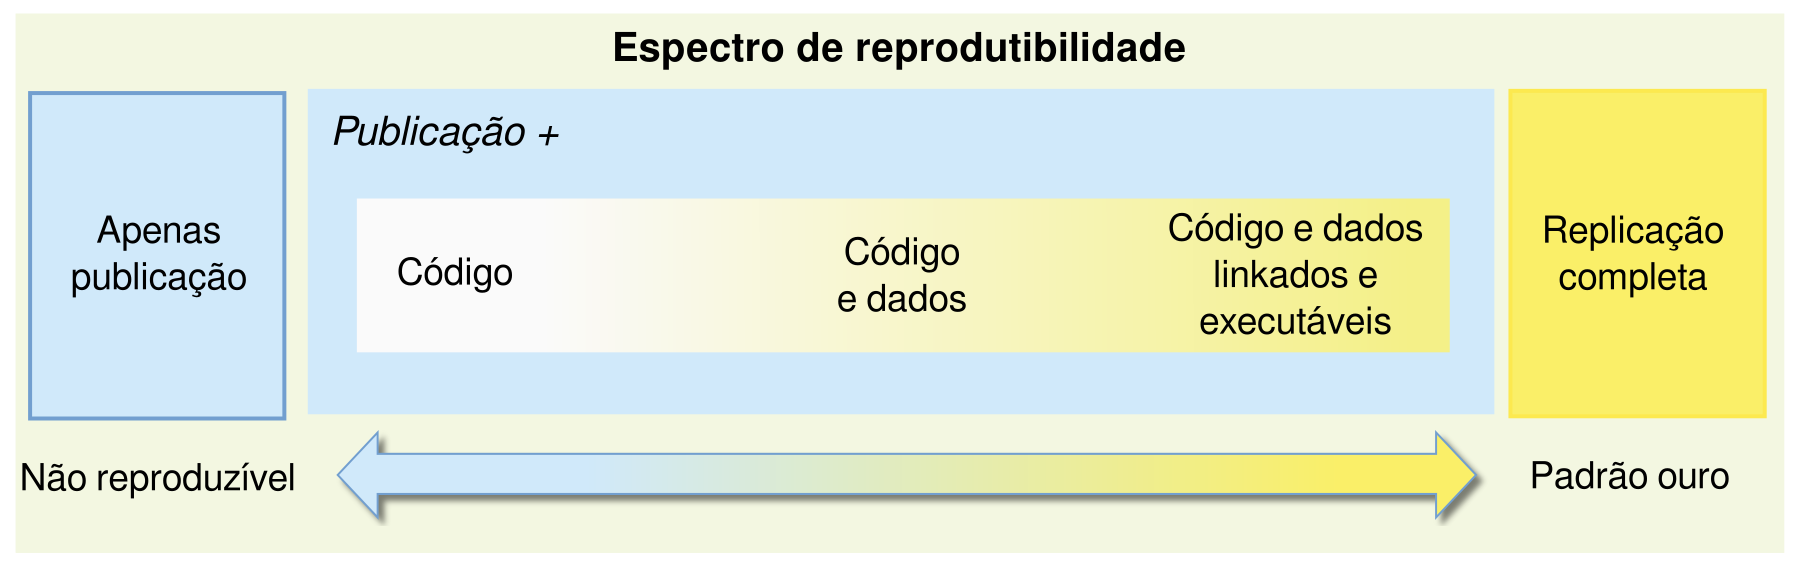
\includegraphics[scale=0.35]{imagens/reproducibility-spectrum-ptbr.png}
  \caption{Espectro de reprodutibilidade \cite{Peng2011}}
  \label{reproducibility-spectrum}
\end{figure}

Apesar das pesquisas reproduzíveis ({\it RR - Reproducible Research}) não
resolverem todos os problemas de validade experimental dos estudos em
engenharia de software, elas ao menos garantem que dados e métodos de análise
estejam disponíveis para inspeção e que os resultados possam ser derivados,
facilitando revisão logo que a publicação acontece. Além disso, é um recurso
valoroso para pesquisadores iniciantes, pesquisas reproduzíveis melhoram o
impacto do próprio estudo, por exemplo, artigos de computação que não
disponibilizam pubicamente dados e códigos possuem menos chances de serem
citados \cite{madeyski2017would}.

A disponibilidade dos softwares científicos tem sido enfatizada também em
discussões sobre sustentabilidade de software, um conceito que diz respeito
à longevidade dos sistemas de software.

%% O surgimento do conteito de engenharia de software baseada em envidências (EBSE
%% - {\it Evidence-Based Software Engineering }) surgiu em um trabalho seminal
%% apresentado em 2004 na {\it International Conference on Software Engineering
%% (ICSE)} e suas ideias e ferramentas, especialmente a revisão sistemática, tem
%% evoluído e amadurecido ao longo do tempo, e tem ajudado a caracterizar e
%% consolidar nosso conhecimento sobre muitos aspectos da pesquisa e práticas da
%% engenharia de software.
%% 
%% Em engenharia de software o termo {\it literatura} foi adicionado formando
%% revisão sistemática de literatura, isto foi feito para evitar confusão com
%% práticas de inspeção de código (comumente definido com o termo revisão) existentes
%% na área.
%% 
%% O objetivo de uma revisão sistemática é buscar e identificar todo material relevante
%% relacionado a um certo tópico (a natureza deste material é determinada pelas
%% questões de pesquisa e a natureza dos participantes intererssados na pesquisa).
%% 
%% Um fator em favor da aceitação dos conceitos da EBSE tem sido a crescente
%% reconhecimento que os resultados de estudos empíricos individuais são frequentemente
%% inconclusivos, e estes tipo de estudos são difícels de replicar com sucesso
%% \cite{sjoberg2005survey}.
%% 
%% Ainda existem poucos estudos replicados \cite{kitchenham2015evidence}.

\section{Sustentabilidade de software} \label{sustentabilidade}

% Software Sustainability: The Modern Tower of Babel

O {\it Dagstuhl Perspective Workshop} é um evento organizado por e para um
pequeno grupo de pesquisadores sêniores de renome internacional, realizado
anualmente na universidade de Dagstuhl\footnote{\url{http://www.dagstuhl.de}}
com o objetivo de refletir sobre o atual estado da ciência da computação.

Através de uma discussão intensiva com foco estratégico o workshop explora
tópicos novos e emergentes da ciência da computação produzindo manifestos que
capturam tendências e desenvolvimentos relacionados aos tópicos explorados.

Realizado desde 2011 o workshop tem explorado diversos tópicos da ciência da
computação, como computação e paleografia, tecnologia da informação como ponte
entre biologia e medicina, métodos de aprendizado de máquina para segurança de
computadores, análise de performance e visualização, entre outros tópicos. Em
sua mais recente edição, o {\it Dagstuhl Perspectives Workshop on ``Engineering
Academic Software''} \cite{allen2017engineering} examinou o estado atual dos
softwares científicos, identificou problemas comuns em seu desenvolvimento,
reconhecimento e sustentabilidade.

Uma das contribuições chave deste workshop é um manifesto contendo um roteiro
para o futuro da engenharia de software profissional e acadêmica, com foco em
instrumentos de suporte para pesquisas em software científico. O manifesto é
expresso em termos de ações ``promessas'' destinado a usuários e
desenvolvedores de softwares científicos, com passos concretos para melhorar o
ambiente em que os softwares são produzidos.

Os compromissos expressados neste manifesto são agrupados em três conceitos gerais:
(i) garantir que softwares científicos sejam {\it citados} apropriadamente;
(ii) promover a {\it carreira} do engenheiro de software desenvolvedor de software científico; e
(iii) medir a qualidade e sustentabilidade do software científico durante e após o seu {\it desenvolvimento}.

No terceiro compromisso, relacionado ao conceito {\it desenvolvimento}, o Dagstuhl Manifesto enfatiza a necessidade de medir a
qualidade e a sustentabilidade dos softwares científicos, e define
sustentabilidade de software como capacidade de perdurar, software sustentável
é aquele que continua a estar disponível no futuro, em novas plataformas e se
atende às novas necessidades \cite{allen2017engineering}.

% campos da engenharia de software, e apesar dos inúmeros entendimentos sobre o
% conceito \cite{venters2014software}, 

Essa definição de sustentabilidade de software é encontrada em mais detalhes no
{\it Karlskrona Manifesto} \cite{becker2014karlskrona}, um documento que alerta
sobre os impactos que os sistemas e a tecnologia da informação causam no futuro
do planeta, convida praticantes e pesquisadores de software a refletir sobre
o tema sustentabilidade na área da ciência da computação.

Sustentabilidade é um conceito guarda chuva composto de múltiplas dimensões, em
sua dimensão técnica, chamada sustentabilidade técnica, temos a preocupação com
a longevidade da informação, dos sistemas, e infraestrutura, e sua adequada
evolução frente as condições do ambiente em constante mudança. Software ocupa
um papel central nessa discussão, ele pode levar a crescentes consumo de
recurso, crescimento da desigualdade social, e influenciar no ganho ou perda de
auto-estima individual.

Se sustentabilidade não for levada em consideração em projetos de software, não
importa qual o domínio ou qual o propósito do software, perde-se a oportunidade
de causar mudanças positivas no planeta e na sociedade.

%Pesquisadores de
%software podem contribuir identificando questões de pesquisa em seu campo para
%ajudar a melhor entender sustentabilidade em projetos de software, Discutir com
%seus pares e pensar sobre como sustentabilidade impacta sua área de pesquisa.
%
%Assim, surge um conjunto de ações que podem ser tomadas pelos diferentes atores
%em direção à garantir sustentabilidade nos projetos de software, ações para
%praticantes de software, pesquisadores, associações profissionais, educadores,
%cientes e usuários.
% 
% 
% Em resumo os dois manifestos, Dagstuhl e Karlskrona, exprimem o conceito de
% sustentabilidade necessários para este estudo, mas é importante citar que
% algumas iniciativas e outros manifestos também estão preocupados com questões
% similares, dentre os quais podemos destacar:
% 
%A ciência aberta e comunidades de pesquisa em software tem sido bastante ativas
%em criar manifestos visando chamadas para ação. Estes manifestos chamam para melhorar
%os softwares e os metadados de bibliografia para citação persistente destes softwares.
%Outros tópicos endereçados nestes manifestos incluem ênfase no acesso ao código fonte.
%
%Agências de financiamento como o {\it US National Science Foundation} estão começando
%a reconhecer produtos de pesquisa como software assim como fazem com as publicações.
%Isto reconhece as contribuições ao softwares assim como primeiro produto de pesquisa.
%
%O {\it Journal of the American Statistical Association (JASA)} irá agora insistir na
%disponibilidade do código e dados durante a revisão dos manuscritos \cite{baker2016scientists}.
%% 
%% \begin{itemize}
%% 
%%   \item Science Code Manifesto \cite{barnes2013science}
%% 
%%     Foco em código fonte escrito especificamente para processar dados de
%%     publicações, afirma que ``todo código fonte escrito especificamente para
%%     processar dados de uma publicação deve estar disponível para os revisores e
%%     leitores do paper''.
%% 
%%   \item FORCE11 Software Citation principles \cite{smith2016software}\footnote{\url{https://www.force11.org/software-citation-principles}}
%% 
%%     Enfatiza persistencia e claridade e diz que ``Software deve ser considerado
%%     um produto legítimo de pesquisas e devem ser possível de serem citados''.
%% 
%%   \item Open Access Pledge \cite{holcombe2011openaccess}\footnote{\url{http://www.openaccesspledge.com}}
%% 
%%     Concentra-se em publicar softwares e papers em locais de {\it open access}.
%% 
%%   \item Open Science Peer Review Oath\footnote{\url{https://f1000research.com/articles/3-271/v2}}
%% 
%%     Concentra-se em potencializar os revisores para exigir acesso aberto aos
%%     softwares, práticas reprodutíveis e revisões transparentes.
%% 
%%   \item UK RSE \cite{ukrse2013}\footnote{\url{http://rse.ac.uk/who}}
%% 
%%     Conscientização sobre a importância e o papel do {\it Research Software
%%     Engineer} através de comunicação e suporta institucional.
%% 
%%   \item Reproducibility manifesto \cite{Barba2012}\footnote{\url{http://lorenabarba.com/gallery/reproducibility-pi-manifesto}}
%% 
%%     Inclui termos para fazer softwares reusáveis por outros. Foco em
%%     reprodutibilidade, deixando sustentabilidade de software fora de questão.
%% 
%%   \item The GeoScience paper of the future initiative \cite{OntoSoft2016}\footnote{\url{http://www.scientificpaperofthefuture.org/gpf/what-is-a-gpf}}
%% 
%%     Possui um conjunto de requerimentos para softwares serem incluidos em
%%     papers.  Focando mais no paper em sí do que no software.
%% 
%%   \item FAIR principles \cite{wilkinson2016fair}\footnote{\url{https://www.nature.com/articles/sdata201618}}
%% 
%%     Foco em dados de pesquisa. O objetivo é fazer eles serem encontráveis,
%%     acessíveis, interoperável e reusável. Estes princípios podem ser
%%     generalizados para aplicar aos softwares.
%% 
%% \end{itemize}

\section{Análise estática de código fonte} \label{analise-estatica}

A análise estática de código fonte é o primeiro passo para coletar informações
necessárias em diversas atividades de verificação, medição e melhoria da
qualidade de produtos de software \cite{Cruz2009, Kirkov2010}. Ela é
realizada com base no código fonte de um programa ou sistema de software, e a
partir daí descobre problemas e propriedades de sua qualidade estrutural
\cite{Chess2007}.

Ferramentas de análise estática estão disponíveis há décadas, em especial,
para programadores. A ferramenta Lint \cite{Johnson1978}, considerada a
primeira ferramenta de análise estática \cite{Gosain2015}, foi criada para
examinar programas escritos em linguagem C e aplicar regras de tipagem mais
estritas do que as regras dos próprios compiladores da linguagem.

%Neste trabalho o nosso interesse reside em compreender características de
%qualidade interna de ferramentas deste domínio de aplicação, do ponto
%de vista de desenvolvedores interessados em manter e evoluir tais ferramentas
%melhorando seus atributos de qualidade interna.
%
%A seção \ref{analise-estatica} apresenta uma definição geral da análise
%estática de código fonte, suas aplicações, sua anatomia, seus formatos de
%representação intermediária e técnicas mais comuns. 

Análise estática de código fonte tem como objetivo prover
informações acerca de um programa a partir do seu código fonte sem
necessidade de execução, e sem requerer qualquer outro artefato do programa
além do próprio código.

É um ramo que possui muitas das suas abordagens em comum com os estudos da
área de análise de programas ({\it program analysis}), especialmente na área de
compiladores, onde atua especialmente nas primeiras etapas do processo de compilação.

A análise estática de código fonte é considerada uma atividade meio com
objetivo de suportar uma variedade de tarefas comuns da engenharia de
software; muitas dessas tarefas são substancialmente úteis em atividades de
manutenção. \citeonline{Binkley2007} define uma lista dessas
atividades, incluindo:

\begin{multicols}{2}
  \begin{itemize}
    \item Análise de performance
    \item Compreensão de programas
    \item Desenvolvimento baseado em modelos
    \item Detecção de clones
    \item Evolução de software
    \item Garantia de qualidade
    \item Localizaçao de falhas
    \item Manutenção de software
    \item Recuperação arquitetural
    \item Testes
  \end{itemize}
\end{multicols}

Seja em qual atividade for, a análise estática possui importância,
pois ao ser capaz de extrair informações diretamente do
código fonte de um programa, pode auxiliar a responder perguntas necessárias
para as diversas atividades de desenvolvimento e evolução de software. Essa
importância se torna ainda mais aparente diante da ``lei'' da tendência para
execução \cite{Harman2010} que indica que todos os tipos de notação tem a
tendência de se tornar executáveis.

\subsection{Usos da análise estática de código fonte} \label{usos}

A análise de programas trata, de modo geral, da descoberta de problemas e
fatos sobre programas, ela pode ser realizada sem a necessidade de executar o
programa (análise estática) ou com informações provenientes de sua execução
(análise dinâmica).

A ideia de que programas de computador podem ser utilizados para analisar
código fonte de outros programas tem uma história de mais de 40 anos.  O
programa PFORT \cite{Ryder1974} foi projetado para localizar potenciais
problemas na portabilidade de código Fortran; em função da diversidade de
dialetos de Fortran, uma compilação sem erros não indicava que o programa
estava correto segundo os padrões da linguagem \cite{Wichmann1995}.

Desde então, ferramentas de análise estática de código fonte têm surgido para
os mais diversos fins -- muitas delas a partir das pesquisas e
desenvolvimentos da área de compiladores.  O {\it parser} utilizado nessas
ferramentas têm funcionalidades análogas aos analisadores usados em
compiladores \cite{Anderson2008}.

O uso de tais ferramentas tem se
tornado mais comum no ciclo de desenvolvimento de
software, sendo aplicadas em uma infinidade de atividades distintas visto que o
campo de aplicação destas ferramentas é bastante variado, cobrindo diferentes
objetivos. De acordo com \citeonline{Chess2007}, as atividades em que análise
estática de código fonte é empregada, destacam-se:

\begin{description}

  \item \textit{Verificação de tipos}. 
    A forma mais amplamente utilizada de análise estática, e uma das quais os
    programadores estão mais familiarizados, é a checagem de tipo.
    Previne que acidentalmente atribuam valores de forma incorreta a
    variáveis. Ainda, ao capturar erros em tempo de compilação, esta checagem
    de tipo previne erros em tempo de execução.

  \item \textit{Verificação de estilo}. 
    Os verificadores de estilo são um tipo de análise estática que aplicam regras
    de forma mais superficial do que os verificadores de tipo. São regras
    relacionadas a espaços em branco, nomes, funções depreciadas, comentários,
    estrutura do programa, entre outros. Os erros reportados por verificadores de
    estilo são aqueles que afetam a leitura e a manutenabilidade do
    código fonte, não indicando potenciais erros em tempo de execução como
    fariam os verificadores de tipo.

  \item \textit{Compreensão de programas}. 
    Ferramentas de compreensão de programa ajudam programadores a terem uma visão
    clara frente a grandes programas de computador, ou seja, programas com
    alto volume de código fonte. Ambientes de desenvolvimento integrados (IDE)
    geralmente incluem funcionalidade de compreensão, por exemplo, ``encontrar
    todos os usos de um certo método'' ou ``encontrar a declaração de uma
    variável global''. Análises mais avançadas chegam a incluir, por exemplo,
    refatoração automática. Estas ferramentas de compreensão também são úteis
    para programadores interessados em entender código fonte escrito por
    outros programadores.

  \item \textit{Verificação de programas}.
    Ferramentas de verificação de programa aceitam como entrada uma especificação
    e um conjunto de código fonte e tenta provar que o código está deacordo
    com a especificação. Quando a especificação é uma descrição completa de
    todo o programa, a ferramenta de verificação poderá realizar uma checagem
    de equivalência para garantir que o código fonte e a especificação
    combinam de forma exata. Programadores raramente têm acesso a uma
    especificação detalhada suficientemente para ser usada numa checagem de
    equivalência, o trabalho de criar esta especificação pode ser maior do que
    o trabalho de escrever o próprio código fonte do programa, desta forma
    este tipo de verificação formal raramente acontece.

  \item \textit{Localização de bugs}. 
    Um localizador de bugs está
    preocupado em apontar locais onde o programa, possivelmente, irá se
    comportar de forma inesperada. A maioria das ferramentas de localização de
    bugs são fáceis de usar porque costumam vir com um conjunto de regras
    ({\it bug idioms}) para descrição de padrões de código que indicam bugs.
    Algumas destas ferramentas costumam usar os mesmos algoritmos utilizados
    por ferramentas de verificação de propriedade.

  \item \textit{Avaliação de segurança}. 
    Ferramentas de análise estática para segurança usam as mesmas técnicas
    encontradas nas outras ferramentas, mas por ter um propósito diferente,
    identificar problemas de segurança, aplicam estas técnicas de forma diferente.
    As primeiras ferramentas de segurança (ITS4, RATS, Flawfinder) eram pouco mais
    do que um {\it ``grep''} melhorado; na maior parte, elas escaneavam o código
    procurando por funções como por exemplo {\it ``strcpy()''} que são
    facilmente usadas de forma inadequada e devem ser inspecionadas
    manualmente no processo de revisão de código fonte.

\end{description}

\subsection{Anatomia da análise de código fonte} \label{anatomia}

Ferramentas de análise estática de código fonte estão organizadas em partes ou
componentes, responsáveis por implementar três funções básicas: a) extração de dados, b) geração de representação
intermediária, e c) análise \cite{Cruz2009, Binkley2007}.

\begin{description}

  \item \textit{Extração de dados}.
    O processo de recuperar dados para futuro processamento ou armazenamento é
    chamado de extração de dados. 

    O primeiro componente da análise de código fonte é a extração de dados,
    responsável por ler o código fonte do programa e gerar uma ou mais
    representações intermediárias. Em essência, este componente converte a sintaxe
    de um programa em uma outra sintaxe abstrata e mais adequada para análise
    posterior.

  \item \textit{Representação intermediária}.
    Exportar os dados extraídos para uma representação intermediária é uma
    estratégia comum para facilitar análise e transformação de dados e
    possivelmente adição de metadados.

    Os dados obtidos na extração precisam ser representados em um formato mais
    abstrato. Esta é a responsabilidade do segundo componente da análise de
    código fonte: armazenar os dados coletados usando uma representação
    intermediária em formato mais adequado para análise automática, abstraindo
    aspectos particulares do programa e da linguagem de programação.

    Alguns tipos de representação intermediária têm sua origem na área de
    compiladores, entre os formatos mais comuns, destacam-se:

    \begin{multicols}{2}
      \begin{itemize}
        \item Árvore sintática abstrata
        \item Grafo de fluxo de controle
        \item Árvore sintática abstrata decorada
        \item Grafo de dependência de módulos
        \item Atribuição estática única
        \item Grafo de dependência de valores
      \end{itemize}
    \end{multicols}

    Estas representações podem ser utilizadas tanto na análise estática quanto
    na análise dinâmica. O uso de um ou outro formato depende do tipo de
    análise e seu propósito. Pode-se combinar diferentes tipos no sentido de
    enriquecer e estruturar a informação extraída.

  \item \textit{Análise}.
    Este componente é responsável por realizar inferências a partir dos dados
    representados internamente. O processo requer que as informações
    armazenadas estejam interconectadas e também interrelacionadas com
    conhecimento anterior. Esta análise pode gerar conhecimento quantitativo
    ou qualitativo, como, por exemplo, métricas de software ou mineração de
    dados, respectivamente. Técnicas de visualização podem ser usadas para
    apoiar este processo.

    Diversas técnicas foram desenvolvidas ao longo do tempo para realizar
    análise, algumas delas são brevemente descritas na seção \ref{tecnicas}.

\end{description}

\subsection{Formatos de representação intermediária} \label{formatos}

Essencialmente, um formato de representação intermediária é uma abstração precisa
das propriedades de um programa representado em um domínio menor. Os
compiladores normalmente constroem esta representação a fim de possuir um
modelo do programa sendo compilado, é comum que compiladores utilizem diversos
formatos durante o curso da compilação.

Em ferramentas de análise estática estes formatos são utilizados durante a
fase de análise para cumprir diversos objetivos, como por exemplo, calcular
métricas de código fonte. A métrica de complexidade ciclomática de McCabe
\cite{McCabe1976}, por exemplo, é definida com base no grafo de fluxo de controle ({\it Control Flow Graph - CFG}) do
programa com o seguinte cálculo $CC = e - n + 2p$. Onde: {\bf e} é o número de
arestas; {\bf n} é o número de nós; e {\bf p} é o número de componentes
fortemente conectados no grafo.

Assim, percebe-se que cada formato de representação intermediária pode ter fins
e objetivos bastante distintos, dentre os formatos mais comuns podemos destacar
\cite{Nielson2015, Stanier2013, Cruz2009, Ramalho1996}:

\begin{description}

  \item \textit{Árvore sintática abstrata}.
    A árvore sintática abstrata (AST - {\it Abstract Syntax Tree}) representa um
    programa tratando os elementos do código fonte como operadores e
    operandos organizados em nós numa árvore, este formato de representação é
    muito popular em tradutores {\it
    source-to-source}\footnote{http://en.wikipedia.org/wiki/Source-to-source\_compiler}.

  \item \textit{Grafo de fluxo de controle}.
    O grafo de fluxo de controle (CFG - {\it Control Flow Graph} ou {\it Call Graph}) é um grafo direcionado
    representando a estrutura de controle de um programa e sua sequência de
    instruções, onde as arestas mostram os possíveis caminhos de execução. Este
    formato é amplamente utilizado em métodos formais para otimização de
    código fonte.

  \item \textit{Grafo de fluxo de dados}.
    O grafo de fluxo de dados (DFG - {\it Data Flow Graph}) é também um grafo
    direcionado onde as arestas representam o fluxo de dados entre as
    operações do programa, este formato pode ser visto como um companheiro do
    grafo de fluxo de controle (CFG) e pode ser gerado ao longo de uma mesma
    análise.

  \item \textit{Árvore sintática abstrata decorada}.
    Árvore sintática abstrata decorada (DAST - {\it Decorated Abstract Syntax Tree}) é
    uma árvore sintática abstrata (AST) melhorada através de um processo de
    definiçao de atributos para os símbolos do programa de forma declarativa
    com uso de uma Gramática de
    Atributos\footnote{https://en.wikipedia.org/wiki/Attribute\_grammar}.

  \item \textit{Grafo de dependência de módulos}.
    O grafo de dependência de módulos (MDG - {\it Module Dependence Graph}) é um grafo
    onde os módulos são representados como nós e as arestas representam as
    relacões entre eles, indicando dependência entre os mesmos.

  \item \textit{Atribuição estática única}.
    Atribuição estática única (SSA - {\it Static Single Assignment}) pode ser vista
    como uma variação ou uma propriedade de outros formatos de representação
    intermediária, é um método que faz cada variável ser atribuída apenas uma única
    vez, facilitando a descoberta de informaçoes sobre os dados representados.

  \item \textit{Grafo de dependência de valores}.
    O grafo de dependência de valores (VDG - {\it Value Dependence Graph}) é uma
    variação que melhora (ao menos para algumas análises) os resultados
    obtidos a partir da atribuição estática única (SSA). Ele representa tanto
    o fluxo de controle quanto o fluxo de dados e assim simplifica a análise.

\end{description}

\subsection{Técnicas de análise} \label{tecnicas}

Inúmeras técnicas e métodos distintos podem ser utilizados pelas ferramentas
de análise estática, seja com o objetivo de verificação de tipos, localização
de bugs, compreensão de programas, avaliação de segurança, ou outra finalidade
qualquer. Segundo \citeonline{German2003, Li2010, Hofer2010} as técnicas e
métodos mais comumente encontrados nas ferramentas atuais são:

\begin{description}

  \item \textit{Análise léxica}.
    A análise léxica é responsável por quebrar o programa em pequenos fragmentos
    (ou {\it tokens}) e verificar se estes fragmentos são palavras válidas
    para uma dada linguagem. A análise léxica não leva em consideração a
    sintaxe do programa, sua semântica ou a interação entre módulos.

  \item \textit{Combinação de padrões de texto}.
    A combinação de padrões de texto ({\it Text-based Pattern Matching}) é a
    maneira mais simples e rápida de procurar vulnerabilidades num código
    fonte.

  \item \textit{Inferência de tipos}.
    A inferência de tipos ({\it Type inference}) refere-se a identificar o
    tipo de variáveis e funções e avaliar se o acesso a elas está em
    conformidade com as regras da linguagem. Linguagens de programação com
    sistema de tipagem incluem mecanismos deste tipo de análise.

  \item \textit{Análise de fluxo de dados}.
    A análise de fluxo de dados ({\it Data flow analysis}) resume-se a coletar
    informação semântica do código fonte do programa, e com métodos algébricos
    deduzir a definição e uso das variáveis em tempo de compilação. O objetivo
    é mostrar que nenhum caminho de execução do programa acessa uma variável
    sem definição ou atribuição prévia.

  \item \textit{Verificação de regra}.
    A verificação de regra ({\it Rule checking}) consiste em checar a segurança
    do programa através de um conjunto de regras pré-estabelecidas.

  \item \textit{Análise de restrição}.
    A análise de restrição ({\it Constraint analysis}) consiste em gerar
    e resolver restrições no processo de análise de um programa.

  \item \textit{Comparação caminho}.
    Comparação caminho ({\it Patch comparison}) inclui comparação de caminho de
    código fonte e de código-binário e é usada principalmente para encontrar
    brechas de vulnerabilidade já ``conhecidas'' e previamente divulgadas por
    fornecedores e praticantes da indústria de software.

  \item \textit{Execução simbólica}.
    A execução simbólica ({\it Symbolic execution}) é usada para representar
    as entradas de um programa através do uso de valores simbólicos ao invés
    de dados reais, produz expressões algébricas sobre a entrada dos símbolos
    do programa durante o processo de implementação e pode detectar
    possibilidade de erros.

  \item \textit{Interpretação abstrata}.
    Interpretação abstrata ({\it Abstract interpretation}) é uma descrição
    formal da análise do programa. Pelo fato de apenas controlar atributos de
    programa de preocupaçao dos usuários, a interpretação da análise semântica
    é similar ao seu significado semântico real.

  \item \textit{Prova de teoremas}.
    Prova de teoremas ({\it Theorem proving}) é baseada na análise semântica do
    programa. Converte o programa em fórmulas lógicas e então tenta provar que
    o programa é um teorema válido usando regras e axiomas.

  \item \textit{Verificação de modelo}.
    O processo de verificação de modelos ({\it Model checking}) primeiro constrói
    um modelo formal do programa tal como uma máquina de estados ou um grafo
    direcionado, então examina e compara o modelo para verificar se o sistema
    cumpre as características pré-definidas. Esta técnica requer a definição e
    descrição das propriedades que devem ser verificados por um pedaço de
    software.

  \item \textit{Verificação formal}.
    Verificação formal ({\it Formal Checking} ou {\it Compliance Analysis}) é o
    processo de provar de forma automatizada que o código do programa está
    correto em relação a uma especificação formal dos seus requisitos.

  \item \textit{Análise de fluxo da informação}.
    Análise de fluxo da informação ({\it Information Flow Analysis}) identifica
    como a execução de uma unidade de código cria dependência entre entradas e
    saídas.

  \item \textit{Verificação de sintaxe}.
    Verificação de sintaxe ({\it Syntax Checks}) tem o objetivo de encontrar
    violação de regras tais como expressões mal-formadas ou fora do padrão.

  \item \textit{Verificação de intervalo}.
    A análise de verificação de intervalo ({\it Range Checking}) tem o objetivo
    de verificar que os valores dos dados permanecem dentro de intervalos
    especificados, bem como manter a precisão especificada.

\end{description}

Diante a variedade e a constante evolução da área de análise estática
\citeonline{Novak2010} fez um estudo propondo uma taxonomia e um conjunto de
dimensões para caracterização de ferramentas de análise estática, mais detalhes
sobre essas dimensões e categorias serão exploradas no Capítulo
\ref{caracterizacao-ferramentas}, no qual apresentaremos uma caracterização de
softwares científicos estudados neste trabalho.

\section{Complexidade estrutural} \label{complexidade}

%% Métricas de software podem ser classificadas em métricas de processo, métricas
%% de projeto e métricas de produto.
%% 
%% Métricas de processo medem atributos relacionados ao ciclo de desenvolvimento
%% e manutenção de software. Métricas de projeto indicam se a execução do
%% processo está progredindo conforme planejado (por exemplo, relação entre o
%% tamanho do software entregue e o esforço total dispendido em seu
%% desenvolvimento).
%% 
%% Métricas de produto medem atributos de produtos e artefatos, como documentos,
%% diagramas, código fonte e arquivos binários. Neste trabalho,
%% apenas métricas de produto serão utilizadas.
%% 
%% Métricas de produto podem ser classificadas em internas (medem propriedades
%% visíveis apenas aos desenvolvedores) ou externas (medem propriedades visíveis
%% aos usuários) \cite{Mohamed1994}.
%% 
%% Neste trabalho, são utilizadas métricas de produto e, especificamente,
%% métricas de código fonte, que cobrem aspectos de tamanho, complexidade e
%% qualidade que podem ser medidos a partir do código fonte de um software.
%% 
%% Métricas de software tem um escopo bastante abrangente, e o termo está
%% associado com muitas atividades da engenharia de software: Medidade e modelos
%% para estimativa de custo e esforço, Coleção de dados, Modelos e medidas de
%% qualidade, Modelos de confiabilidade, Métricas de segurança, Métricas
%% estruturais e de complexidade, Avaliação de maturidade de capacidade,
%% Gerenciamento através de métricas, Avaliação de métodos e ferramentas.
%% 
%% \subsection{Métricas de código fonte} \label{metricas-de-codigo}
%% 
%% As propriedades visíveis aos desenvolvedores podem ser medidas através de
%% métricas de código fonte. A observação e o monitoramento de seus valores podem
%% indicar aspectos relevantes à manutenibilidade de um programa. Dentre as
%% inúmeras métricas de código fonte nosso interesse está em métricas que indicam
%% características relevantes à modularidade de um produto de software,
%% complexidade estrutural e custo de mudança.

%Structural and Complexity Metrics
%Desirable quality attributes like reliability and maintainability cannot be
%measured until some operational version of the code is available. Yet, we
%wish to be able to predict which parts of the software system are likely to be
%less reliable, more difficult to test, or require more maintenance than oth-
%ers, even before the system is complete. As a result, we measure structural
%attributes of representations of the software that are available in advance
%of (or without the need for) execution; then, we try to establish empiri-
%cally predictive theories to support quality assurance, quality control, and
%quality prediction. These representations include control flow graphs that
%usually model code and various unified modeling language (UML) dia-
%grams that model software designs and requirements. Structural metrics
%can involve the arrangement of program modules, for example, the use
%and properties of design patterns. These models and related metrics are
%described in Chapter 9.

Do ponto de vista de métricas, neste trabalho, estamos interessados, de fato, na métrica
de complexidade estrutural SC ({\it Structural Complexity}), uma medida da
complexidade de projetos de sistema de software proposta por
\citeonline{Darcy2005} como indicador da complexidade dos sistemas de software
em relação à sua estrutura interna e ao relacionamento entre os seus
componentes.

Complexidade é um tema bastante amplo, e para compreender onde os
sistemas de softwares se encaixam neste contexto precisamos definir brevemente
o que vem a ser sistemas complexos.

Sistemas complexos são sistemas no qual grandes redes de componentes sem
controle central dão origem a um comportamento
coletivo complexo, com processamento sofisticado de informação, e adaptação
através de aprendizado ou evolução \cite{Mitchell2009}. As seguintes
características são comuns a todos os sistemas complexos:

\begin{description}

  \item[Comportamento coletivo complexo.] Apesar de serem compostos por
  elementos bastante simples individualmente, sistemas complexos podem exibir
  comportamentos coletivos bastante sofisticados.

  \item[Troca de sinais e processamento de informação.] Em cada um destes
  sistemas, seus componentes individuais consomem e produzem informação entre
  si. Parte do comportamento do sistema envolve transformação dessa informação.

  \item[Adaptação.] Sistemas complexos adaptam-se a novas situações de forma a
  aumentar suas chances de sobrevivência diante de novas condições em seu
  ambiente.

\end{description}

Os sistemas complexos podem ser classificados como naturais ou artificiais, os
sistemas naturais são aqueles cuja constituição não tem participação humana, ao
contrário dos sistemas artificiais que são projetados por humanos, com
objetivos e funções previamente definidos \cite{Simon1996}. Neste sentido,
sistemas de software podem ser caracterizados como sistemas complexos
artificiais, pois exibem comportamento coletivo complexo, realizam trocas de
sinais e processamento de informação e passam por adaptação para se adequar a
mudanças em seu ambiente.

Sistemas de software são compostos por componentes, em geral, chamados de
módulos, que possuem tanto estado quanto comportamento próprios,
módulos individuais de um sistema de software são simples quando comparados com
o sistema como um todo. Módulos produzem informação para outros módulos
através de parâmetros em chamadas de sub-rotinas e consomem informação através
dos valores de retornos destas chamadas. O fluxo contínuo de novos requisitos e
de mudanças no ambiente operacional de sistemas de software força-os a se
manter em constante evolução em busca de “sobrevivência”.

Esta medida é, possivelmente, um indicativo de problemas na manutenibilidade de
sistemas de software, em especial sobre o esforço necessário para atividades de
manutenção \cite{Terceiro2012}. Ela está relacionada a como os módulos de um
programa estão organizados bem como à estrutura interna de cada módulo. Esta
métrica pode dar indícios importantes sobre características arquiteturais de um
programa de software e pode explicar seus atributos de qualidade interna.

%Modularity
%Modularity describes the logical partitioning of software into several parts, components, and modules.
%Software will be easy to understand and change when composed of independent modules.
%“A Software Maintainability Evaluation Methodology”, 1981
%\cite{kumar2012survey}

%Faz um experimento usando CBO LCOM e outras metricas como preditor de manutenabilidade...
%\cite{Dagpinar2003}

%A complexidade de um sistema de software pode ser de três tipos: a complexidade
%do problema, a complexidade procedural, e a complexidade do projeto do sistema.
%Esta última é o foco deste trabalho.
%A complexidade do problema está relacionada ao domínio do problema.
%A complexidade procedural está relacionada à estrutura lógica da programa, em es-
%pecial do seu comprimento, em termos de número de tokens, linhas de código fonte, ou
%estruturas de controle. Este último tipo é o que iremos estudar neste trabalho.
%
%Os sistemas complexos podem naturais ou artificiais, uma colônia de formigas
%por exemplo pode ser caracterizado como um sistema complexo natural, onde
%individualmente cada formiga se apresenta como criatura relativamente simples,
%com instintos básicos como procurar alimento, responder a estímulos químicos
%vindos de outras formigas, combater intrusos, etc. No entanto, quando
%observadas coletivamente em uma colônia, as formigas aparentam ser muito mais
%sofisticadas. Elas são capazes de se organizar em diferentes atividades, criar
%estruturas complexas dentro de seu formigueiro, e de encontrar o caminho mais
%curto para uma fonte de alimento.
%
%Os sistemas naturais são aqueles cuja constituição não tem participação humana.
%Sistemas artificiais são projetados por humanos, com objetivos e funções
%definidos.  Sistemas artificiais podem ou não serem projetados à imagem de um
%sistema natural, e durante a sua concepção eles são discutidos em termos tanto
%de suas características (o que eles são) como de necessidades que eles devem
%satisfazer (o que eles deveriam ser) \cite{Simon1996}.
%
%É importante ressaltar que esta caracterização de sistemas de software como
%sistemas complexos diz respeito à estrutura interna dos sistemas, ou seja, aos
%componentes que o constituem e ao relacionamento entre estes componentes. Não
%foram considerados outros aspectos importantes de sistemas complexos, como por
%exemplo o seu relacionamento com o ambiente externo.
%
%como uma combinação das métricas de acoplamento (CBO) e coesão (LCOM4), 
%
%Sistemas de software, no entanto, se
%diferenciam dos sistemas complexos naturais pelo fato de serem projetados;
%consequentemente, o seu processo evolucionário não é intrinsecamente parte do
%seu comportamento, mas fruto da ação consciente de seus desenvolvedores.
%
%\cite{Tegarden1995}
%
%"The implication of this result is that, when
%designing, implementing, and maintaining software to control complexity, both coupling and cohesion should be considered jointly,
%instead of independently" Darcy 2005
%
%Many studies have demonstrated a significant correlation between
%LOC and the cyclomatic number. The researchers usually suggest that
%this correlation proves that cyclomatic number increases with size; that
%is, larger code is more complex code. However, careful interpretation of
%the measures and their association reveals only that the number of deci-
%sions increases with code length, a far less profound conclusion. The cyclo-
%matic number may be just another size measure. Chapter 9 contains more
%detailed discussion of validation for the McCabe measures.
%
%{\bf SC} {\it Structural Complexity (Complexidade estrutural)}: mede a
%complexidade do software \cite{Darcy2005} combinando os valores de CBO e LCOM4.

\citeonline{Darcy2005} definem complexidade estrutural como uma combinação de
acoplamento e coesão. Estes são dois conceitos complementares: enquanto o
acoplamento reflete o relacionamento entre módulos, a coesão nos fornece uma
visão da organização dos componentes internos de um módulo e seus
relacionamentos.

Uma formalização da métrica proposta por \citeonline{Darcy2005} pode ser
expressa da seguinte maneira, para um projeto $p$ e seu conjunto de módulos
$M(p)$, a complexidade estrutural $SC(p)$ de $p$ é:

\begin{equation}
SC(p) = \frac
{ \displaystyle \sum_{m \in M(p)} CBO(m) \times LCOM4(m) }
{ |M(p)| }
\end{equation}

Esta medida de complexidade estrutural é portanto a complexidade
estrutural média entre todos os módulos do sistema.

\begin{itemize}

  \item {\bf CBO} {\it Coupling Between Objects (Acoplamento entre objetos)}:
    mede o acoplamento entre objetos do software \cite{Chidamber1994}
    calculando em nível de classe o número total de acessos à outras classes do
    mesmo sistema, é comum ser também chamada de Fan-out da classe. CBO é então
    definida pela seguinte fórmula:

\begin{equation}
\label{formula-cbo}
CBO(C) = \sum_{i=1}^{n} cliente(C, Ci)
\end{equation}

Onde:

\begin{equation}
cliente(Ci, Cj) =
  \begin{cases}
    1 \text{ se } Ci \Rightarrow Cj \wedge Ci \neq Cj \\
    0 \text{ caso contrario} \\
  \end{cases}
\end{equation}

A notação $ Ci \Rightarrow Cj $ indica acesso à atributos, variáveis, métodos ou funções
entre módulos ou classes.

Apesar de ser possível formalizar a métrica CBO através da fórmula acima, sua descriçao original é
bastante complexa, levando à implementações variadas do seu cálculo
\cite{Lincke2008}. A definição original, por exemplo, inclui explicitamente
acoplamento via herança \cite{Harrison1998}, no entando não deixa claro como
deve ser tratado métodos herdados \cite{Briand1999}. A definição original
afirma também que apenas chamadas explícitas (e não chamadas implicitas) de
construtores são contabilizadas. Algumas definições de CBO incluem não apenas $
cliente(Ci, Cj) $ mas também a recíproca $ cliente(Cj, Ci) $ de forma que o valor
final inclui classes que ela acessa somado ao número de classes do sistema que
a acessam \cite{Sant2008}.

Quanto mais as classes forem independentes, mais fácil é reutilizá-las e menos
arriscado é modificá-las. Classes mais acopladas precisam de mais rigor em
testes, pois mais partes do sistema dependem delas.

  \item {\bf LCOM4} {\it Lack of Cohesion in Methods (Ausência de coesão em
    métodos)}: mede o grau de falta de coesão em métodos \cite{Hitz1995}.

O cálculo de LCOM4 é dado através de grafo não-orientado em que os nós ou
vértices são os métodos e atributos de uma classe e as arestas são acessos à
métodos e atributos. O cálculo desta métrica pode ser formalizado como a
seguir \cite{Silva2012}.

Seja $ X $ uma classe qualquer e $ M_x $ o conjunto de métodos desta classe,
considere um grafo simples não-orientado $ G_x(V, E) $, sendo:

\begin{equation}
V = M_x
\text{ e }
E = \{ \langle m, n \rangle \in V \times V \}
\end{equation}

Onde:
\begin{equation}
(\exists i \in Ix : (m \text{ accessos } i) \land (n \text{ accessos } i)) \lor (m \text{ chamadas } n) \lor (n \text{ chamadas } m)
\end{equation}

O valor da métrica LCOM4 para uma classe $ X $ é então definido como o número
de componentes conectados do grafo $ G_x (1 \leq LCOM(x) \geq | M_x |)$.

Coesão entre os métodos de uma classe é uma propriedade desejável, portanto o
valor ideal para esta métrica é 1. Se uma classe tem diferentes conjuntos de
métodos não relacionados entre si, é um indício de que a classe deveria ser
refatorada em classes menores e mais coesas.

\end{itemize}


%------------------------------------------%

\xchapter{Revisão estruturada}{}

Copiar localmente todos os artigos em formato PDF de todas as edições das
conferências SCAM - Source Code Analysis and Manipulation Working
Conference\footnote{http://www.ieee-scam.org} e ASE - Automated Software
Engineering\footnote{http://ase-conferences.org}.

Acessar o cada edição do evento e fazer cópia local de
cada artigo, armazenar os artigos separados por edição, uma pasta para
cada ano.

Segue os títulos de todos os artigos analisados.

%# Papers tools da conferencia estao no IEEE Xplore?
%
%(enviei em 16/nov email para os chairs da trilha ferramentas do SCAM 2014
%perguntando onde encontro os papers da trilha ferramentas)
%
%17/11 - Foutse Khomh respondeu informando que no IEEEXplore tem tudo,
%incluindo os tools papers.
%
%uma leitura superficial
%para encontrar referencia e link sobre ferramenta desenvolvida
%resultou nos seguintes papers com ferramenta disponível livremente:
%
%SCAM 2010/05601817.pdf Wrangler (OK) - mas erlang nao pode ser analisado
%
%9 novas ferramentas, verificar qual linguagem é utilizada em cada uma delas:
%
%* Wrangler        | erlang
%
%Podemos analizar todas exceto Wrangler em erlang, então são 9 ferramentas.
%Somando a ferramenta SourceMeter encontrada no levantamento anterior dos anos
%2001, 2002, 2013, 2014. Temos total de 9 ferramentas da academia para anlisar.


\section{SCAM - Source Code Analysis and Manipulation Working Conference}

Todos os artigos em formato PDF foram obtidos de forma manual através da área
da
conferência\footnote{http://ieeexplore.ieee.org/xpl/conhome.jsp?punumber=1000715}
no IEEE Xplore.

\subsection{SCAM 2001}

http://ieeexplore.ieee.org/xpl/mostRecentIssue.jsp?punumber=7667

\begin{enumerate}[itemsep=-1ex]
  \item A Case Study in Detecting Software Security Vulnerabilities using Constraint Optimization
  \item A Hybrid Program Slicing Framework
  \item An Object Level Transformation Technique to Improve the performance of Embedded Applications
  \item A source-to-source compiler for generating dependable software
  \item Analysis and Manipulation of Distributed Multi-Language Software Code
  \item Application Maintenance Using Software Agents
  \item Detecting Dead Statements for Concurrent Programs
  \item Finding Code on the World Wide Web: A Preliminary Investigation
  \item Flow Insensitive Points-to Sets
  \item Identifying Clones in the Linux Kernel
  \item JMangler – A Framework for Load-Time Transformation of Java Class Files
  \item Library Transformations
  \item Measurement and Analysis of Runtime Profiling Data for Java Programs
  \item Preserving the Documentary Structure of Source Code in Language-based Transformation Tools
  \item Program Slicing: Methods and Applications
  \item Restructuring Web Applications via Transformation Rules
  \item Smell the Coffee! Uncovering Java Analysis Issues
  \item Software Engineering by Source Transformation - Experience with TXL
  \item Static Slicing and Parametric Polymorphism
  \item The Formal Transformation Approach to Source Code Analysis and Manipulation
  \item Type Infeasible Call Chains
  \item Using Automated Source Code Analysis For Software Evolution
  \item Using Data Flow Analysis to Infer Type Information in Java Bytecode
\end{enumerate}

\subsection{SCAM 2002}

\begin{enumerate}[itemsep=-1ex]
  \item Parallel Support for Source Code Analysis and Modification
  \item Towards Measurement of Testability of Concurrent Object-Oriented Programs using Fault Insertion: A Preliminary Investigation
  \item An Extensible Metrics Extraction Environment for Object-oriented Programming Languages
  \item Evaluating Clone Detection Tools for Use during Preventative Maintenance
  \item A Simple Mathematically Based Framework for Rule Extraction Using Wide Spectrum Language
  \item VADA: A Transformation-based System for Variable Dependence Analysis
  \item Combining source transformation and operator overloading techniques to compute derivatives for MATLAB programs
  \item Mechanized Operational Semantics of WSL
  \item Handling Preprocessor-Conditioned Declarations
  \item Grammar Programming in TXL
  \item An Interprocedural amorphous slicer for WSL
  \item Dynamic Slicing Object-Oriented Programs for Debugging
  \item Construction of the System Dependence Graph for Web Application Slicing
  \item Predicate-Based Dynamic Slicing of Message Passing Programs
  \item Using Dependence Graphs as a Support to Document Programs
  \item Precise Call Graph Construction in the Presence of Function Pointers
  \item Semantics Guided Filtering of Combinatorial Graph Transformations in Declarative Equation-Based Languages
  \item Visualization of Exception Propagation for Java using Static Analysis
\end{enumerate}

\subsection{SCAM 2003}

http://ieeexplore.ieee.org/xpl/mostRecentIssue.jsp?punumber=8773

\begin{enumerate}[itemsep=-1ex]
  \item (listar o nome dos artigos aqui)
\end{enumerate}

\subsection{SCAM 2004}

http://ieeexplore.ieee.org/xpl/mostRecentIssue.jsp?punumber=9523

\begin{enumerate}[itemsep=-1ex]
  \item (listar o nome dos artigos aqui)
\end{enumerate}

\subsection{SCAM 2005}

http://ieeexplore.ieee.org/xpl/mostRecentIssue.jsp?punumber=10344

\begin{enumerate}[itemsep=-1ex]
  \item (listar o nome dos artigos aqui)
\end{enumerate}

\subsection{SCAM 2006}

http://ieeexplore.ieee.org/xpl/mostRecentIssue.jsp?punumber=4026839

\begin{enumerate}[itemsep=-1ex]
  \item (listar o nome dos artigos aqui)
\end{enumerate}

\subsection{SCAM 2007}

http://ieeexplore.ieee.org/xpl/mostRecentIssue.jsp?punumber=4362882

\begin{enumerate}[itemsep=-1ex]
  \item (listar o nome dos artigos aqui)
\end{enumerate}

\subsection{SCAM 2008}

http://ieeexplore.ieee.org/xpl/mostRecentIssue.jsp?punumber=4637522

\begin{enumerate}[itemsep=-1ex]
  \item (listar o nome dos artigos aqui)
\end{enumerate}

\subsection{SCAM 2009}

http://ieeexplore.ieee.org/xpl/mostRecentIssue.jsp?punumber=5279860

\begin{enumerate}[itemsep=-1ex]
  \item (listar o nome dos artigos aqui)
\end{enumerate}

\subsection{SCAM 2010}

http://ieeexplore.ieee.org/xpl/mostRecentIssue.jsp?punumber=5600365

\begin{enumerate}[itemsep=-1ex]
  \item (listar o nome dos artigos aqui)
\end{enumerate}

\subsection{SCAM 2011}

http://ieeexplore.ieee.org/xpl/mostRecentIssue.jsp?punumber=6063701

\begin{enumerate}[itemsep=-1ex]
  \item (listar o nome dos artigos aqui)
\end{enumerate}

\subsection{SCAM 2012}

http://ieeexplore.ieee.org/xpl/mostRecentIssue.jsp?punumber=6389882

\begin{enumerate}[itemsep=-1ex]
  \item (listar o nome dos artigos aqui)
\end{enumerate}

\subsection{SCAM 2013}

http://ieeexplore.ieee.org/xpl/mostRecentIssue.jsp?punumber=6636284

\begin{enumerate}[itemsep=-1ex]
  \item Empirical Investigation of SEA-Based Dependence Cluster Properties
  \item Characterization and Assessment of the Linux Configuration Complexity
  \item Criticality of Defects in Cyclic Dependent Components
  \item Code Clustering Workbench
  \item ForkSim: Generating Software Forks for Evaluating Cross-Project Similarity Analysis Tools
  \item Empirical Evidence of Large-Scale Diversity in API Usage of Object-Oriented Software
  \item Aspectual Source Code Analysis with GASR
  \item Driving a Sound Static Software Analyzer with Branch-and-Bound
  \item PtrTracker: Pragmatic Pointer Analysis
  \item Tracing with a Minimal Number of Probes
  \item A State Alteration and Inspection-based Interactive Debugger
  \item Proteum/FL: a Tool for Localizing Faults using Mutation Analysis
  \item GeCoS: A Framework for Prototyping Custom Hardware Design Flows
  \item Review Efforts Reduction by Partitioning of Static Analysis Warnings
  \item JSN OSE : Detecting JavaScript Code Smells
  \item Determining Dynamic Coupling in JavaScript Using Object Type Inference
  \item CodeMetropolis – code visualisation in MineCraft
  \item MetricMiner: Supporting Researchers in Mining Software Repositories
  \item Assembler Restructuring in FermaT
  \item A Hidden Markov Model to Detect Coded Information Islands in Free Text
  \item Fix-it: An Extensible Code Auto-Fix Component in Review Bot
  \item sql-schema-comparer: Support of Multi-Language Refactoring with Relational Databases
  \item A Relational Symbolic Execution Algorithm for Constraint-Based Testing of Database Programs
  \item Ontological Interpretation of Object-Oriented Programming Abstractions
\end{enumerate}

\subsection{SCAM 2014}

http://ieeexplore.ieee.org/xpl/mostRecentIssue.jsp?punumber=6970367

\begin{enumerate}[itemsep=-1ex]
  \item Effect of clone information on the performance of developers fixing cloned bugs
  \item Automatic Identification of Important Clones for Refactoring and Tracking
  \item A Comparative Study of Bug Patterns in Java Cloned and Non-cloned Code
  \item A Change-Type Based Empirical Study on the Stability of Cloned Code
  \item C/C++ Thread Safety Analysis
  \item Toolset and Program Repository for Code Coverage- Based Test Suite Analysis and Manipulation
  \item The E KEKO /X Program Transformation Tool
  \item Flowgen: Flowchart-Based Documentation Framework for C++
  \item PESTO: A Tool for Migrating DOM-based to Visual Web Tests
  \item Pangea: A Workbench for Statically Analyzing Multi-Language Software Corpora
  \item Total ADS: Automated Software Anomaly Detection System
  \item ACUA: API Change and Usage Auditor
  \item Bulk Fixing Coding Issues and Its Effects on Software Quality: Is It Worth Refactoring?
  \item Instrumentation of Annotated C Programs for Test Generation
  \item Scalable Security Verification of Software at Compile Time
  \item Impact of Code Refactoring Using Object-Oriented Methodology on a Scientific Computing Application
  \item Concolic Fault Abstraction
  \item On the Accuracy of Forward Dynamic Slicing and Its Effects on Software Maintenance
  \item Efficient Utilization of Secondary Storage for Scalable Dynamic Slicing
  \item SENSA: Sensitivity Analysis for Quantitative Change-Impact Prediction
  \item Seeing Is Slicing: Observation Based Slicing of Picture Description Languages
  \item Explaining Why Methods Change Together
  \item Studying Fine-Grained Co-evolution Patterns of Production and Test Code
  \item Supplementary Bug Fixes vs. Re-opened Bugs
  \item Semantic Versioning versus Breaking Changes: A Study of the Maven Repository
  \item Fast Flow Analysis with Godel Hashes
  \item A Parallel On-Demand Algorithm for Computing Interprocedural Dominators
  \item Are Object Graphs Extracted Using Abstract Interpretation Significantly Different from the Code?
  \item Bit-Level Taint Analysis
  \item Pruning, Pushdown Exception-Flow Analysis
  \item On Automatically Generating Commit Messages via Summarization of Source Code Changes
  \item On the Use of Context in Recommending Exception Handling Code Examples
  \item A Pattern Search Method for Unpreprocessed C Programs Based on Tokenized Syntax Trees
  \item Identifying Source Code Reuse across Repositories Using LCS-Based Source Code Similarity
\end{enumerate}

\subsection{SCAM 2015}

http://ieeexplore.ieee.org/xpl/mostRecentIssue.jsp?punumber=7321933

\begin{enumerate}[itemsep=-1ex]
  \item (listar o nome dos artigos aqui)
\end{enumerate}


\section{ASE - Automated Software Conference}

Até o ano de 1996 a conferencia se chamava KBSE - Knowledge-Based Software
Engineering Conference

http://ieeexplore.ieee.org/xpl/conhome.jsp?punumber=1000410

A partir de 1997 passou a se chamar ASE - Automated Software Conference.

http://ieeexplore.ieee.org/xpl/conhome.jsp?punumber=1000064

\subsection{ASE/KBSE 1991}

http://ieeexplore.ieee.org/xpl/mostRecentIssue.jsp?punumber=5069

\begin{enumerate}[itemsep=-1ex]
  \item A Knowledge-based Interface To Promote Software Understanding
  \item Domain-specific Representations In The KBSA Concept Demo
  \item LARGE Software System Maintenance
  \item A Learning-based Software Engineering Environment
  \item Active Assistance For Domain Modeling
  \item Using Domain Knowledge To Synthesize Routing Software
  \item Implementation Of An Activity Coordination System
  \item Domain Modeling - Evolving Research
  \item Lockheed Environment For Automatic Programming
  \item A Knowledge-based Approach To Software System Understanding
  \item CTPLAN: A Planning-based Approach To Automatically Detecting Flaws In Concurrent Algorithms
  \item Composite System Design: The Good News And The Bad News
  \item The KBSA Requirements/specification Facet: ARIES
  \item Acquiring Software Design Schemas: A Machine Learning Perspective
  \item Analogical Matching For Specification
  \item Rule Chaining In MARVEL: Dynamic Binding Of Parameters
  \item KBRAS: Knowledge-based Requirements Acquisition System
  \item Directions For Future KBSA Research
  \item Representation And Maintenance of process knowledge for large Scale Systems development
  \item The Role Of Analogy In Specification Derivation
  \item Encouraging The Adoption Of KBSE Technology: What Needs To Happen First?
  \item Sharing And Reuse Of Requirements Knowledge
  \item Motivating Adoption Of KBSA: Issues, Arguments, And Strategies
  \item A Knowledge And Deduction Based Software Retrieval Tool
  \item Functional Representation And Program Debugging
  \item Requirement Directed Automatic Instrumentation Generation For Program Monitoring And Measuring
  \item The Knowledge-based Software Assistant: A Program Summary
  \item Complex Objects In Knowledge-based Requirement Engineering
\end{enumerate}

\subsection{ASE/KBSE 1992}

http://ieeexplore.ieee.org/xpl/mostRecentIssue.jsp?punumber=421

\begin{enumerate}[itemsep=-1ex]
  \item A knowledge-based software development environment for scientific model-building
  \item Domain-oriented design environments
  \item Prototyping VDM specifications with KIDS
  \item Program concept recognition
  \item Software synthesis shell SOFTEX/S
  \item A code synthesis experiment
  \item Towards a logic-based reconstruction of software configuration management
  \item Track assignment in an air traffic control system: a rational reconstruction of system design
  \item Educating knowledge-based software engineers
  \item Explorations on the formal frontier of distributed system design
  \item Reusing database queries in analogical domains
  \item Automatic composition of data structures to represent relations
  \item Transformation of a semi-formal specification to VDM
  \item Knowledge-based constraint-driven software synthesis
  \item Knowledge-based support for scientific programming
  \item DoD's software technology plans: what do they mean for KBSE, and what does it mean for them?
  \item A knowledge-based software process library for process-driven software development
  \item Simulating the Gries/Dijkstra design process
  \item Software reuse through view type clusters
  \item Efficiently computing derived performance data
  \item Program understanding-does it offer hope for aging software?
  \item Domain abstractions in requirements engineering: an exemplar approach?
  \item Managing design knowledge to provide assistance to large-scale software development
  \item Software design by reusing architectures
  \item CAESAR: a system for case based software reuse
\end{enumerate}

\subsection{ASE/KBSE 1993}

http://ieeexplore.ieee.org/xpl/mostRecentIssue.jsp?punumber=921

\begin{enumerate}[itemsep=-1ex]
  \item A knowledge based framework for developing and customizing schedulers
  \item Articulation: an integrated approach to the diagnosis, replanning, and rescheduling of software process failures
  \item An experiment in applying knowledge-based software engineering technology
  \item The knowledge base maintenance assistant
  \item Validation of rule-based reactive systems by sound scenario generalization
  \item Development of an expert assistant for software evaluation using a hybrid approach
  \item A common architecture to encourage reuse of natural language/text processing tools
  \item The ARIES Simulation Component (ASC)
  \item Inquire: predicate-based use and reuse
  \item A knowledge base for software test refinement
  \item GRIT-an extended REFINE for more executable specifications
  \item Diagrams for software synthesis
  \item An analogy-based retrieval mechanism for software design reuse
  \item Transformational approach to transportation scheduling
  \item Observations on using empirical studies on developing a knowledge-based software engineering tool
  \item Towards supporting design phase synthesis
  \item An implementation of bounded obligations
  \item Accelerating browsing by automatically inferring a user's search goal
  \item Operations for evolving specifications
  \item Interactive elaboration of generic designs
  \item Knowledge requirements for the automatic generation of project management reports
\end{enumerate}

\subsection{ASE/KBSE 1994}

http://ieeexplore.ieee.org/xpl/mostRecentIssue.jsp?punumber=995

\begin{enumerate}[itemsep=-1ex]
  \item Software technology risk advisor
  \item Critical success factors for knowledge-based software engineering applications
  \item An augmented pattern matcher as a tool to synthesize conceptual descriptions of programs
  \item Knowledge-based risk assessment and cost estimation
  \item Using machine learning to synthesize search programs
  \item A cooperative program understanding environment
  \item A formal approach to reusing more general components
  \item A formal approach to domain-oriented software design environments
  \item Integrating object-oriented paradigms and logic programming: the OPLA language
  \item User interface design assistance for large-scale software development
  \item Agent-based support for communication between developers and users in software design
  \item Graphical support for code-level software understanding
  \item A flexible rule-chaining engine for process-based software engineering
  \item Composing reusable software components through views
  \item Abstract data structure recognition
  \item Intelligent assistance for software construction: a case study
  \item Evolution and reuse of formal specifications using decision structures
  \item Systematic incremental validation of rule-based reactive systems
  \item A framework for distributed system designs
  \item Task-oriented and similarity-based retrieval
  \item Formal specification tools for test coverage analysis
  \item Application of REFINE Language Tools to software quality assurance
  \item AMPHION: automatic programming for subroutine libraries 
\end{enumerate}

\subsection{ASE/KBSE 1995}

http://ieeexplore.ieee.org/xpl/mostRecentIssue.jsp?punumber=3518

\begin{enumerate}[itemsep=-1ex]
  \item Searching for a global search algorithm
  \item An empirical evaluation of KBSA technology
  \item Test sequences as plans: an experiment in using an AI planner to generate system tests
  \item Automating changes of data type in functional programs
  \item Towards an epistemology for software representations
  \item Classification and retrieval of reusable components using semantic features
  \item A transformation system for interactive reformulation of design optimization strategies
  \item Legal issues in knowledge-based software engineering
  \item An interface between different software development environments
  \item Specification and animation of a bank transfer
  \item Towards high-level deductive program synthesis based on type theory
  \item Interactive explanation of software systems
  \item Classifying software components using design characteristics
  \item From object-oriented to knowledge-based programming (NUT system development experience)
  \item Domain-oriented software process re-engineering with software synthesis shell SOFTEX/S
  \item META-AMPHION: synthesis of efficient domain-specific program synthesis systems
  \item A model for decision maintenance in the WinWin collaboration framework
  \item Knowledge-based program synthesis for a geometric constraint satisfaction system
  \item Application of a decision support mechanism to the business rules lifecycle
  \item CACHET: an interactive, incremental-attribution-based program transformation system for deriving incremental programs
  \item Portability by automatic translation a large-scale case study
  \item Representing object models as theories
  \item Logical frameworks as a basis for verification tools: a case study 
\end{enumerate}

\subsection{ASE/KBSE 1996}

http://ieeexplore.ieee.org/xpl/mostRecentIssue.jsp?punumber=4065

\begin{enumerate}[itemsep=-1ex]
  \item Constructing transition models of AI planner behavior
  \item Applying plan recognition algorithms to program understanding
  \item Integrating software process models and design rationales
  \item Addressing complexity, coordination, and automation in software development with the KBSA/ADM
  \item Extending design environments to software architecture design
  \item Complementing semi-formal specifications with Z
  \item Trusting your assistant
  \item Using knowledge-based transformations to reverse-engineer COBOL programs
  \item Set differentiation: a method for the automatic generation of filtering algorithms
  \item Synthesis of local search algorithms by algebraic means
  \item Deductive synthesis of numerical simulation programs from networks of algebraic and ordinary differential equations
  \item Knowledge-based re-engineering of legacy programs for robustness in automated design
  \item A knowledge-based toolkit for software visualisation
  \item Software synthesis for trade-off design
  \item Synthesis of schedulers for planned shutdowns of power plants 
\end{enumerate}

\subsection{ASE 1997}

http://ieeexplore.ieee.org/xpl/mostRecentIssue.jsp?punumber=5003

\begin{enumerate}[itemsep=-1ex]
  \item Mapping software architectures to efficient implementations via partial evaluation
  \item TESS: automated support for the evolution of persistent types
  \item Application of formal methods to the development of a software maintenance tool
  \item Interactive component-based software development with Espresso
  \item Automatic synthesis of recursive programs: the proof-planning paradigm
  \item Correct-schema-guided synthesis of steadfast programs
  \item Modelling the application domains of software engineering technologies
  \item Reactive system validation using automated reasoning over a fragment library
  \item Strategies of structural synthesis of programs
  \item Precise specification and automatic application of design patterns
  \item An automated object-oriented testing for C++ inheritance hierarchy
  \item On the verification of VDM specification and refinement with PVS
  \item Facilitating an automated approach to architecture-based software reuse
  \item A static analysis for program understanding and debugging
  \item Mechanising requirements engineering: reuse and the application of domain analysis technology
  \item Modeling software processes by using process and object ontologies
  \item A contribution to program comprehension by program analysis: application to numerical programs
  \item Specification and verification of the Co4 distributed knowledge system using LOTOS
  \item Processing natural language requirements
  \item Enhancing the component reusability in data-intensive business programs through interface separation
  \item Research directions for automated software verification: using trusted hardware
  \item Data flow analysis within the ITOC information system design recovery tool
  \item Exploiting domain-specific knowledge to refine simulation specifications
  \item Automated configuration of distributed applications from reusable software architectures
  \item Towards semantic-based object-oriented CASE tools
  \item Moving proofs-as-programs into practice
  \item Feedback handling in dynamic task nets
  \item Genetic algorithms for dynamic test data generation
  \item Formally specifying engineering design rationale
  \item NORA/HAMMR: making deduction-based software component retrieval practical
  \item Using KIV to specify and verify architectures of knowledge-based systems
  \item Tools supporting the creation and evolution of software development knowledge
  \item Augmenting abstract syntax trees for program understanding
  \item Declarative specification of software architectures
  \item A structured approach for synthesizing planners from specifications
  \item From formal specifications to natural language: a case study
  \item Retrieving software components that minimize adaptation effort
  \item A metric-based approach to detect abstract data types and state encapsulations
  \item Distributed cooperative formal methods tools
  \item Applying concept formation methods to object identification in procedural code
  \item Formal specification of human-computer interaction by graph grammars under consideration of information resources
  \item Towards a design assistant for distributed embedded systems
  \item Modular flow analysis for concurrent software
  \item Automatic high-quality reengineering of database programs by temporal abstraction
  \item A formal automated approach for reverse engineering programs with pointers
  \item Extracting objects from legacy imperative code
  \item Notes on refinement, interpolation and uniformity
\end{enumerate}

\subsection{ASE 1998}

http://ieeexplore.ieee.org/xpl/mostRecentIssue.jsp?punumber=5935

\begin{enumerate}[itemsep=-1ex]
  \item ASSISTing exit decisions in software inspection
  \item Towards the automated debugging and maintenance of logic-based requirements models
  \item Task oriented software understanding
  \item Automated software test data generation for complex programs
  \item Statically checkable design level traits
  \item An empirical study of the evolution of a software system
  \item An automated approach for supporting software reuse via reverse engineering
  \item Testing using log file analysis: tools, methods, and issues
  \item Synthesizing software architecture descriptions from Message Sequence Chart specifications
  \item Requirements engineering and verification using specification animation
  \item The very idea of software development environments: a conceptual architecture for the arts' environment paradigm
  \item On detecting and handling inconsistencies in integrating software architecture design and performance evaluation
  \item Identifying pre-conditions with the Z/EVES theorem prover
  \item Schema-guided synthesis of constraint logic programs
  \item Automating UI generation by model composition
  \item ADLscope: an automated specification-based unit testing tool
  \item Explanation based scenario generation for reactive system models
  \item Dowsing: a tool framework for domain-oriented browsing of software artifacts
  \item Component-based software process support
  \item Reusability hypothesis verification using machine learning techniques: a case study
  \item A coordination system approach to software workflow process evolution
  \item Parameterising (algebraic) specifications on diagrams
  \item Automated knowledge acquisition and application for software development projects
  \item Automated integrative analysis of state-based requirements
  \item An automated framework for structural test-data generation
  \item A tool for automated system analysis based on modular specifications
  \item Planware-domain-specific synthesis of high-performance schedulers
  \item Detection of exclusive OR global predicates
  \item From Z to BON/Eiffel
  \item A visualization concept for hierarchical object models
  \item Developing the designer's toolkit with software comprehension models
  \item Planning equational verification in CCS
  \item Don't verify, abstract!
  \item Explaining synthesized software
  \item Management of evolving specifications using category theory
  \item Development, assessment, and reengineering of language descriptions
  \item Illustrating object-oriented library reuse by example: a tool-based approach
  \item Specification-based testing of Ada units with low encapsulation
  \item Brewing fresh Java from legacy Lisp-an experiment in automated reverse engineering
  \item A design pattern based approach to generating synchronization adaptors from annotated IDL
  \item A configurable automatic instrumentation tool for ANSI C
  \item Programmatic testing of the Standard Template Library containers
  \item Towards a theory for integration of mathematical verification and empirical testing
  \item Specification-based browsing of software component libraries 
\end{enumerate}

\subsection{ASE 1999}

http://ieeexplore.ieee.org/xpl/mostRecentIssue.jsp?punumber=6516

\begin{enumerate}[itemsep=-1ex]
  \item Modular and incremental analysis of concurrent software systems
  \item Siddhartha: a method for developing domain-specific test driver generators
  \item Fixing some transformation problems
  \item Implementing effective automatic cryptographic protocol analysis
  \item Combining fault avoidance, fault removal and fault tolerance: an integrated model
  \item Beyond components-connections-constraints: dealing with software architecture difficulties
  \item Applying test automation to type acceptance testing of telecom networks: a case study with customer participation
  \item AML: an Architecture Meta-Language
  \item A formal ontology for re-use of software architecture documents
  \item An integration of deductive retrieval into deductive synthesis
  \item An approach to automatic code generation for safety-critical systems
  \item A comparative study between linear programming verification (LPV) and other verification methods
  \item An approach to software requirements elicitation using precepts from activity theory
  \item Verification of picture generated code
  \item Enhancing annotation visibility for software inspection
  \item An automatic and optimized test generation technique applying to TCP/IP protocol
  \item Component-based systems as an aid to design validation
  \item Automatic synthesis of control software for an industrial automation control system
  \item Towards adaptive web agents
  \item Separating concerns in direct manipulation user interfaces
  \item Towards automatic imperative program synthesis through proof planning
  \item vUML: a tool for verifying UML models
  \item Evolving object-oriented designs with refactorings
  \item Automatic proofs of properties of simple C-- modules
  \item Exploration harnesses: tool-supported interactive discovery of commercial component properties
  \item NAVCo: negotiation-based adaptive view coordination
  \item Automatically detecting mismatches during component-based and model-based development
  \item A metric based technique for design flaws detection and correction
  \item A visualization tool for constraint program debugging
  \item Automatic generation of test oracles: from pilot studies to application
  \item Deductive synthesis of event-based software architectures
  \item Automatically structuring textual requirement scenarios
  \item Data mining library reuse patterns in user-selected applications
  \item Automatic software clustering via Latent Semantic Analysis
  \item Automated translation of UML models of architectures for verification and simulation using SPIN
  \item Dynamic accommodation of change: automated architecture configuration of distributed systems
  \item Towards discovery, specification, and verification of component usage
  \item Retrenchment: extending the reach of refinement
  \item An ML editor based on proofs-as-programs
  \item Industrial applications of software synthesis via category theory
  \item System for automated validation of embedded software in multiple operating configurations
  \item Rule-based strategic reflection: observing and modifying behaviour at the architectural level
  \item UNA based iterative test data generation and its evaluation
  \item Architectural element matching using concept analysis
  \item Development of a constraint-based airlift scheduler by program synthesis from formal specifications
  \item UMLAUT: an extendible UML transformation framework
  \item An overview of Lutess a specification-based tool for testing synchronous software
  \item Controlled natural language can replace first-order logic
  \item Software test generation using refinement types
  \item Advanced modelling and verification techniques applied to a cluster file system 
\end{enumerate}

\subsection{ASE 2000}

http://ieeexplore.ieee.org/xpl/mostRecentIssue.jsp?punumber=7013

\begin{enumerate}[itemsep=-1ex]
  \item An overview of a method and its support tool for generating B specifications from UML notations
  \item Automatic derivation of Petri net based distributed specification with optimal allocation of resources
  \item Controlled automation of consistency enforcement
  \item Semantic abstraction rules for class diagrams
  \item Automated security checking and patching using TestTalk
  \item Using Little-JIL to coordinate agents in software engineering
  \item New visual interface for engineering use case models
  \item A group critic system for object-oriented analysis and design
  \item Non-interference analysis for mixed criticality code in avionics systems
  \item Towards explicit representation of architectural design assumptions
  \item Automating the composition of middleware configurations
  \item Generating test data for branch coverage
  \item A DSL approach to improve productivity and safety in device drivers development
  \item Specialization patterns
  \item Simultaneous checking of completeness and ground confluence
  \item Model checking programs
  \item Translating use cases to sequence diagrams
  \item Mutation operators for specifications
  \item A transformational viewpoint on design patterns
  \item Combining the best attributes of qualitative and quantitative risk management tool support
  \item Practical large scale what-if queries: case studies with software risk assessment
  \item Computing interfaces in Java
  \item Java model checking
  \item $\pi$-SPACE: a formal architecture description language based on process algebra for evolving software systems
  \item Test sequences generation from LUSTRE descriptions: GATEL
  \item A declarative approach for designing and developing adaptive components
  \item Identification of potentially infeasible program paths by monitoring the search for test data
  \item Exploring the design of an intentional naming scheme with an automatic constraint analyzer
  \item The use of abduction and recursion-editor techniques for the correction of faulty conjectures
  \item Issues for the automatic generation of safety critical software
  \item Exploring and validating the contributions of real-world knowledge to the diagnostic performance of automated database design tools
  \item Extending UML to support domain analysis
  \item Circular coinductive rewriting
  \item Management of change in structured verification
  \item An experiment in scientific program understanding
  \item Using graph rewriting to specify software architectural transformations
  \item Formal construction of the Mathematically Analyzed Separation Kernel
  \item A comparison of questionnaire-based and GUI-based requirements gathering
  \item Representing technology to promote reuse in the software design process
  \item CM-Builder: an automated NL-based CASE tool
  \item Toward the automatic assessment of evolvability for reusable class libraries
  \item Finding comparatively important concepts between texts
  \item Upgrading legacy instances of reactive systems
  \item Renaming detection 
\end{enumerate}

\subsection{ASE 2001}

http://ieeexplore.ieee.org/xpl/mostRecentIssue.jsp?punumber=7763

\begin{enumerate}[itemsep=-1ex]
  \item Design rationale for software maintenance
  \item Higher order function synthesis through proof planning
  \item Automatic test data generation for programs with integer and float variables
  \item Enforcing business policies through automated reconfiguration
  \item Automated software engineering using concurrent class machines
  \item A tool for lazy verification of security protocols
  \item The synthesis of a Java card tokenisation algorithm
  \item Scalable consistency checking between diagrams - the VIEWINTEGRA approach
  \item A new way of automating statistical testing methods
  \item Automatically restructuring programs for the Web
  \item A concurrency test tool for Java monitors
  \item Modeling class operations in B: Application to UML behavioral diagrams
  \item Developing generative frameworks using XML
  \item A UML validation toolset based on abstract state machines
  \item Generating EDI message translations from visual specifications
  \item Action Language Verifier
  \item Acceptance based assurance
  \item Amphion/NAV: deductive synthesis of state estimation software
  \item Adequate reverse engineering
  \item Automatic verification of Java design patterns
  \item Certifying domain-specific policies
  \item Monitoring programs using rewriting
  \item Verify properties of mobile code
  \item Tailoring a COTS group support system for software requirements inspection
  \item Automated conversion from a requirements document to an executable formal specification
  \item Providing early feedback in the development cycle through automated application of model checking to software architectures
  \item Static consistency checking for distributed specifications
  \item Connectors synthesis for deadlock-free component based architectures
  \item Towards an evolutionary formal software development
  \item Shared variables interaction diagrams
  \item Strategies for automated specification-based testing of synchronous software
  \item Security specification and verification
  \item AGATE, access graph based tools for handling encapsulation
  \item TestEra: a novel framework for automated testing of Java programs
  \item Generation of functional test sequences from B formal specifications presentation and industrial case-study
  \item Wins and losses of algebraic transformations of software architectures
  \item Better reasoning about software engineering activities
  \item Unfriendly COTS integration - instrumentation and interfaces for improved plugability
  \item Semi-automated verification of Erlang code
  \item Specification modeling and validation applied to a family of network security products
  \item Programs are abstract data types
  \item Enhancing partial-order reduction via process clustering
  \item Tracing execution of software for design coverage
  \item Automated validation of software models
  \item Program execution based module cohesion measurement
  \item Automated test-data generation from formal models of software
  \item Automated check of architectural models consistency using SPIN
  \item Test purposes: adapting the notion of specification to testing
  \item Modeling and verification of distributed real-time systems based on CafeOBJ
  \item Implementation of specification conjunction and domain interaction in Rosetta
  \item An automated tool for analyzing Petri nets using Spin
  \item Exploiting heap symmetries in explicit-state model checking of software
  \item Model checking for an executable subset of UML
  \item Context-aware browsing of large component repositories
  \item Composition and refinement of behavioral specifications
  \item Model-checking real-time concurrent systems
  \item Automating the performance and reliability analysis of enterprise information systems
  \item Generation of distributed system test-beds from high-level software architecture descriptions
  \item Automatic translation from UML specifications to B
  \item Formally testing fail-safety of electronic purse protocols
  \item Combining static analysis and model checking for software analysis
  \item A technique for mutation of Java objects
  \item Identification of high-level concept clones in source code
  \item Instantiating and detecting design patterns: putting bits and pieces together
  \item An analysis-revision cycle to evolve requirements specifications
  \item Automata-based verification of temporal properties on running programs
  \item Towards a precise definition of the OMG/MDA framework
  \item Knowledge base approach to consistency management of UML specifications 
\end{enumerate}

\subsection{ASE 2002}

http://ieeexplore.ieee.org/xpl/mostRecentIssue.jsp?punumber=8183

\begin{enumerate}[itemsep=-1ex]
  \item SeDiTeC-testing based on sequence diagrams
  \item Dependence management for dynamic reconfiguration of component-based distributed systems
  \item A model of planning and enactment support in complex software development projects
  \item From early requirements to user interface prototyping: a methodological approach
  \item Adding value to formal test oracles
  \item No Java without caffeine: A tool for dynamic analysis of Java programs
  \item Generating product-lines of product-families
  \item Towards usable and relevant model checking techniques for the analysis of dependable interactive systems
  \item A temporal logic approach to the specification of reconfigurable component-based systems
  \item CpprofJ: aspect-capable call path profiling of multi-threaded Java applications
  \item Report on the workshop on the state of the art in automated software engineering
  \item Experience report on automated procedure construction for deductive synthesis
  \item A framework for automatic debugging
  \item An approach to rapid prototyping of large multi-agent systems
  \item Predicting software stability using case-based reasoning
  \item Process support for tools interoperability
  \item What makes finite-state models more (or less) testable?
  \item Semantic links and co-evolution in object-oriented software development
  \item Interfaces for modular feature verification
  \item Automatic test case optimization using a bacteriological adaptation model: application to .NET components
  \item VIATRA - visual automated transformations for formal verification and validation of UML models
  \item Combining and adapting software quality predictive models by genetic algorithms
  \item Distributed modular model checking
  \item Generative design patterns
  \item Knowledge-based synthesis of numerical programs for simulation of rigid-body systems in physics-based animation
  \item Automatic verification of any number of concurrent, communicating processes
  \item Automating requirements traceability: Beyond the record \& replay paradigm
  \item Monitoring requirements: a case study
  \item Automatic synthesis of distributed systems
  \item Analyzing dependencies in large component-based systems
  \item On CASE tool usage at Nokia
  \item Automated validation of class invariants in C++ applications
  \item Generating test data for functions with pointer inputs
  \item Towards certifying domain-specific properties of synthesized code
  \item Constructing CORBA-supported oracles for testing: a case study in automated software testing
  \item Adapting applications on the fly
  \item Deviation analysis through model checking
  \item System testing for object-oriented frameworks using hook technology
  \item Enabling iterative software architecture derivation using early non-functional property evaluation
  \item Automatic inter-procedural test case generation
  \item Identifying cause and effect relations between events in concurrent event-based components
  \item Automatic validation of deployed J2EE components using aspects
  \item Model-based tests of truisms
  \item Systematic bridging the gap between requirements and OO design
  \item Assumption generation for software component verification
  \item Generating expected results for automated black-box testing 
\end{enumerate}

\subsection{ASE 2003}

http://ieeexplore.ieee.org/xpl/conhome.jsp?punumber=1000064

\begin{enumerate}[itemsep=-1ex]
  \item VUML: a viewpoint oriented UML extension
  \item Model-based verification of Web service compositions
  \item Refactoring C with conditional compilation
  \item On the automatic evolution of an OS kernel using temporal logic and AOP
  \item A model-driven approach to non-functional analysis of software architectures
  \item Automatic generation of content management systems from EER-based specifications
  \item Debugging overconstrained declarative models using unsatisfiable cores
  \item Visual specification of concurrent systems
  \item Architecture style-based calculi for non-functional properties
  \item XRay views: understanding the internals of classes
  \item Automated environment generation for software model checking
  \item Automated software testing using a metaheuristic technique based on Tabu search
  \item Automating component adaptation for reuse
  \item An approach for tracing and understanding asynchronous architectures
  \item Analysis of inconsistency in graph-based viewpoints: a category-theoretical approach
  \item Fault localization with nearest neighbor queries
  \item Testing database transaction concurrency
  \item Automatically inferring concern code from program investigation activities
  \item Automation for exception freedom proofs
  \item Semi-automatic fault localization and behavior verification for physical system simulation models
  \item Specification and synthesis of hybrid automata for physics-based animation
  \item Graph rewriting and transformation (GReAT): a solution for the model integrated computing (MIC) bottleneck
  \item An incremental approach to task-specific information delivery in SE processes
  \item An infrastructure to support meta-differencing and refactoring of source code
  \item What test oracle should I use for effective GUI testing?
  \item A Java component model for evolving software systems
  \item Unspeculation
  \item Extending diagnosis to debug programs with exceptions
  \item Automated requirements-based generation of test cases for product families
  \item Parallel breadth-first search LTL model-checking
  \item Certifying measurement unit safety policy
  \item Visual constraint diagrams: runtime conformance checking of UML object models versus implementations
  \item Aspectizing server-side distribution
  \item Model checking software requirement specifications using domain reduction abstraction
  \item An empirical study on groupware support for software inspection meetings
  \item Deriving user interface requirements from densely interleaved scientific computing applications
  \item Tool-assisted unit test selection based on operational violations
  \item Overview of OpenModel-based validation with partial information
  \item A type system for statically detecting spreadsheet errors
  \item Depiction and playout of multi-threaded program executions
  \item SPQR: flexible automated design pattern extraction from source code
  \item Generating design pattern detectors from pattern specifications
  \item A pragmatic study of binary class relationships
  \item A new structural coverage criterion for dynamic detection of program invariants
  \item Detecting requirements interactions: a three-level framework
  \item Applying AutoBayes to the analysis of planetary nebulae images
  \item Predicting fault prone modules by the Dempster-Shafer belief networks
  \item The feature signatures of evolving programs
  \item DeCo: a declarative coordination framework for scientific model federations
  \item Automating relative debugging
  \item Test suite design for code generation tools
  \item A programmable client-server model: robust extensibility via DSLs
  \item Communicating requirements using end-user GUI constructions with argumentation
  \item Theoretical foundations of updating systems
\end{enumerate}

\subsection{ASE 2004}

http://ieeexplore.ieee.org/xpl/mostRecentIssue.jsp?punumber=9305

\begin{enumerate}[itemsep=-1ex]
  \item Establishment of automated regression testing at ABB: industrial experience report on 'avoiding the pitfalls'
  \item ScriptEase: generative design patterns for computer role-playing games
  \item Combining the box structure development method and CSP
  \item Adaptable concern-based framework specialization in UML
  \item RCAT: a performance analysis tool
  \item CodeCrawler - polymetric views in action
  \item Evaluating clone detection techniques from a refactoring perspective
  \item Modeling and simulation of context-aware mobile systems
  \item Test-suite reduction for model based tests: effects on test quality and implications for testing
  \item Automated support for framework selection and customization
  \item Instant and incremental transformation of models
  \item Collaborative tools for mobile requirements acquisition
  \item A scalable approach to user-session based testing of Web applications through concept analysis
  \item Verifying interactive Web programs
  \item Validating personal requirements by assisted symbolic behavior browsing
  \item Automatic method completion
  \item Using a structure-based configuration tool for product derivation
  \item Automating traceability for generated software artifacts
  \item Refactoring use case models on episodes
  \item Property-oriented test generation from UML Statecharts
  \item Rostra: a framework for detecting redundant object-oriented unit tests
  \item Modeling behavior in compositions of software architectural primitives
  \item T-UPPAAL: online model-based testing of real-time systems
  \item Analyzing interaction orderings with model checking
  \item A computational framework for supporting software inspections
  \item Automated analysis of timing information in UML diagrams
  \item Automated data mapping specification via schema heuristics and user interaction
  \item Evaluation of tool support for architectural evolution
  \item An environment for building a system out of its requirements
  \item Verifiable concurrent programming using concurrency controllers
  \item CHET: a system for checking dynamic specifications
  \item The education of a software engineer
  \item Requirements monitoring for service-based systems: towards a framework based on event calculus
  \item Automated dynamic reconfiguration using AI planning
  \item Parameterized interfaces for open system verification of product lines
  \item From testing to diagnosis: an automated approach
  \item A differencing algorithm for object-oriented programs
  \item ScriptEase: generating scripting code for computer role-playing games
  \item Architecture for generating Web-based, thin-client diagramming tools
  \item Aspect mining using event traces
  \item A statistical model to locate faults at input levels
  \item Helping object-oriented framework use and evaluation by means of historical use information
  \item Mapping template semantics to SMV
  \item Interactive visualization of concurrents programs [concurrents read concurrent]
  \item On-the-fly generation of k-path tests for C functions
  \item Data-mining synthesised schedulers for hard real-time systems
  \item Experiences integrating and scaling a performance test bed generator with an open source CASE tool
  \item Modeling Web-based dialog flows for automatic dialog control
  \item Inferring specifications to detect errors in code
  \item Using transient/persistent errors to develop automated test oracles for event-driven software
  \item A dataflow language for scriptable debugging
  \item Consistency checking in an infrastructure for large-scale generative programming
  \item Heuristic search with reachability tests for automated generation of test programs
  \item COMPASS: tool-supported adaptation of interactions
  \item A case study in JML-based software validation
  \item Automated performance validation of software design: an industrial experience
  \item A case study of coverage-checked random data structure testing
  \item Understanding aspects via implicit invocation
  \item Using a genetic algorithm and formal concept analysis to generate branch coverage test data automatically
  \item Combination model checking: approach and a case study
  \item Context-aware code certification
  \item ISPIS: a framework supporting software inspection processes
  \item Decision support for test management in iterative and evolutionary development
  \item Formal framework for automated analysis and verification of Web-based applications 
  \item Group support for distributed collaborative concurrent software modeling
\end{enumerate}

\subsection{ASE 2005}

http://dl.acm.org/citation.cfm?id=1101908\&CFID=841024589\&CFTOKEN=75079163

\begin{enumerate}[itemsep=-1ex]
  \item The power of software
  \item Virtual humans: lessons learned in integrating a large-scale AI project
  \item Designing and implementing a family of intrusion detection systems
  \item Exploiting predicate structure for efficient reachability detection
  \item Application of design for verification with concurrency controllers to air traffic control software
  \item Efficient temporal-logic query checking for presburger systems
  \item A component model for internet-scale applications
  \item Automating the performance management of component-based enterprise systems through the use of redundancy
  \item UMLDiff: an algorithm for object-oriented design differencing
  \item Identifying traits with formal concept analysis
  \item Precise identification of composition relationships for UML class diagrams
  \item On dynamic feature location
  \item Blowtorch: a framework for firewall test automation
  \item An analysis of rule coverage as a criterion in generating minimal test suites for grammar-based software
  \item Automatic test factoring for java
  \item ClassSheets: automatic generation of spreadsheet applications from object-oriented specifications
  \item Generation of visual editors as eclipse plug-ins
  \item Clearwater: extensible, flexible, modular code generation
  \item Secure sharing between untrusted users in a transparent source/binary deployment model
  \item Automating experimentation on distributed testbeds
  \item AMNESIA: analysis and monitoring for NEutralizing SQL-injection attacks
  \item Timna: a framework for automatically combining aspect mining analyses
  \item A parameterized interpreter for modeling different AOP mechanisms
  \item A generic approach to supporting diagram differencing and merging for collaborative design
  \item Visualization-based analysis of quality for large-scale software systems
  \item Automatic verification of design patterns in Java
  \item Optimized run-time race detection and atomicity checking using partial discovered types
  \item Reasoning about real-time statecharts in the presence of semantic variations
  \item Automated replay and failure detection for web applications
  \item Locating faulty code using failure-inducing chops
  \item Empirical evaluation of the tarantula automatic fault-localization technique
  \item Automated test generation for engineering applications
  \item Let's agree to disagree
  \item A similarity-aware approach to testing based fault localization
  \item Process support to help novices design software faster and better
  \item The PLUSS toolkit?: extending telelogic DOORS and IBM-rational rose to support product line use case modeling
  \item A strategy for efficient verification of relational specifications, based on monotonicity analysis
  \item Quasi-random testing
  \item Constraint-based test data generation in the presence of stack-directed pointers
  \item QoS-aware dynamic service composition in ambient intelligence environments
  \item A visual language and environment for composing web services
  \item Learning to verify branching time properties
  \item Simon: modeling and analysis of design space structures
  \item Lattice-based adaptive random testing
  \item A unified fitness function calculation rule for flag conditions to improve evolutionary testing
  \item A threat-driven approach to modeling and verifying secure software
  \item Automated path generation for software fault localization
  \item EA-Miner: a tool for automating aspect-oriented requirements identification
  \item yagg: an easy-to-use generator for structured test inputs
  \item Determining the cost-quality trade-off for automated software traceability
  \item A uniform deductive approach for parameterized protocol safety
  \item A component-based development framework for supporting functional and non-functional analysis in control system design
  \item A rigorous approach for proving model refactorings
  \item Compositional reasoning for port-based distributed systems
  \item Model-based self-monitoring embedded programs with temporal logic specifications
  \item Specialization and extrapolation of software cost models
  \item NFRs-aware architectural evolution of component-based software
  \item Code security analysis with assertions
  \item Data mining and cross-checking of execution traces: a re-interpretation of Jones, Harrold and Stasko test information
  \item Properties and scopes in web model checking
  \item Synthesis of correct and distributed adaptors for component-based systems: an automatic approach
  \item A context-sensitive structural heuristic for guided search model checking
  \item Test input generation for red-black trees using abstraction
  \item Testing in resource constrained execution environments
  \item Prufrock: a framework for constructing polytypic theorem provers
  \item Bamboo: an architecture modeling and code generation framework for configuration management systems
  \item Using communicative acts in high-level specifications of user interfaces for their automated synthesis
  \item A tool for automatic UML model consistency checking
  \item Automated population of causal models for improved software risk assessment
  \item Introduction to doctoral symposium
  \item Automated generation of testing tools for domain-specific languages
  \item Constructing interaction test suites with greedy algorithms
  \item Verifying the correctness of hume programs: an approach combining deductive and algorithmic reasoning
  \item A model transformation approach to automatic model construction and evolution
  \item Formal support for merging and negotiation
  \item In regression testing selection when source code is not available
  \item Specification and automated processing of security requirements (SAPS'05)
  \item Software security assurance tools, techniques and metrics (SSATTM)
  \item 3rd international workshop on traceability in emerging forms of software engineering (TEFSE 2005)
  \item Software certificate management (SoftCeMent'05)
  \item 2nd Workshop on the state of the art in automated software engineering
\end{enumerate}

\subsection{ASE 2006}

http://ieeexplore.ieee.org/xpl/mostRecentIssue.jsp?punumber=4019543

\begin{enumerate}[itemsep=-1ex]
  \item Verifying Specifications with Proof Scores in CafeOBJ
  \item Winning the DARPA Grand Challenge: A Robot Race through the Mojave Desert
  \item Automatic Property Checking for Software: Past, Present and Future
  \item Automated Information Aggregation for Scaling Scale-Resistant Services
  \item Generating Domain-Specific Visual Language Editors from High-level Tool Specifications
  \item An Automated Formal Approach to Managing Dynamic Reconfiguration
  \item Differencing and Merging of Architectural Views
  \item An Empirical Comparison of Automated Generation and Classification Techniques for Object-Oriented Unit Testing
  \item Command-Form Coverage for Testing Database Applications
  \item Automatic Identification of Bug-Introducing Changes
  \item Modularity Analysis of Logical Design Models
  \item A Portable Compiler-Integrated Approach to Permanent Checking
  \item Integrating and Scheduling an Open Set of Static Analyses
  \item Reverse Engineering of Design Patterns from Java Source Code
  \item ArchTrace: Policy-Based Support for Managing Evolving Architecture-to-Implementation Traceability Links
  \item Automating Software Traceability in Very Small Companies: A Case Study and Lessons Learne
  \item Bogor/Kiasan: A k-bounded Symbolic Execution for Checking Strong Heap Properties of Open Systems
  \item Security Analysis of Crypto-based Java Programs using Automated Theorem Provers
  \item Accurate Centralization for Applying Model Checking on Networked Applications
  \item Using Decision Trees to Predict the Certification Result of a Build
  \item Managing the Complexity of Large Free and Open Source Package-Based Software Distributions
  \item Concurrent Engineering support in Software Engineering
  \item Mining Aspects from Version History
  \item Identifying Refactorings from Source-Code Changes
  \item Sieve: A Tool for Automatically Detecting Variations Across Program Versions
  \item From Capability Specifications to Code for Multi-Agent Software
  \item An Instant Message-Driven User Interface Framework for Thin Client Applications
  \item Using communicative acts in interaction design specifications for automated synthesis of user interfaces
  \item Annotation Inference for Safety Certification of Automatically Generated Code (Extended Abstract)
  \item A Unified Model for Product Data Management and Software Configuration Management
  \item Human-Friendly Line Routing for Hierarchical Diagrams
  \item Contradiction Finding and Minimal Recovery for UML Class Diagrams
  \item Programming Language Inherent Support for Constrained XML Schema Definition Data Types and OWL DL
  \item A methodology for automated test generation guided by functional coverage constraints at specification level
  \item An Automated Approach for Goal-driven, Specification-based Testing
  \item Effective Generation of Interface Robustness Properties for Static Analysis
  \item Automatic Generation of Detection Algorithms for Design Defects
  \item Software Library Usage Pattern Extraction Using a Software Model Checker
  \item Automated Round-trip Software Engineering in Aspect Weaving Systems
  \item Towards Automatic Assertion Refinement for Separation Logic
  \item Automated Reasoning on Aspects Interactions
  \item Detecting Precedence-Related Advice Interference
  \item Round-Trip Engineering of Framework-Based Software using Framework-Specific Modeling Languages
  \item Integrated Variability Modeling of Features and Architecture in Software Product Line Engineering
  \item Software Connectors for Highly Distributed and Voluminous Data Intensive Systems
  \item Coverage Metrics to Measure Adequacy of Black-Box Test Suites
  \item Management of Incomplete and Inconsistent Views
  \item Energy-Awareness in Distributed Java-Based Software Systems
  \item LSS: A Tool for Large Scale Scenarios
  \item A new web browser including a transferable function to Ajax codes
  \item Tobias-Z: An executable formal specification of a test generator
  \item Model-driven Monitoring: Generating Assertions from Visual Contracts
  \item The Rearranger - A New Assembler Utility
  \item TOPCASED Combining Formal Methods with Model-Driven Engineering
  \item UML-based Service Discovery Tool
  \item Automated Verification Tool for DHTML
  \item Mock-object generation with behavior
  \item Domain-specific Model Checking Using The Bogor Framework
  \item Testing Tools and Techniques: A Mini-Tutorial on Evaluation Methods for ASE
\end{enumerate}

\subsection{ASE 2007}

http://dl.acm.org/citation.cfm?id=1321631\&CFID=841024589\&CFTOKEN=75079163

\begin{enumerate}[itemsep=-1ex]
  \item Exploring the neighborhood with dora to expedite software maintenance
  \item Netstub: a framework for verification of distributed java applications
  \item Modeling bug report quality
  \item Diconic addition of failsafe fault-tolerance
  \item Ensuring consistency in long running transactions
  \item Assertion-based repair of complex data structures
  \item Automatic code stylizing
  \item Keyword programming in java
  \item Towards supporting awareness of indirect conflicts across software configuration management workspaces
  \item Combined static and dynamic mutability analysis
  \item Sequential circuits for program analysis
  \item Residual dynamic typestate analysis exploiting static analysis: results to reformulate and reduce the cost of dynamic analysis
  \item Directed test generation using symbolic grammars
  \item Nighthawk: a two-level genetic-random unit test data generator
  \item An aspect-oriented weaving mechanism based on component and connector architecture
  \item Towards automatic model synchronization from model transformations
  \item An automated model-based debugging approach
  \item Context-aware statistical debugging: from bug predictors to faulty control flow paths
  \item Object ownership profiling: a technique for finding and fixing memory leaks
  \item Parseweb: a programmer assistant for reusing open source code on the web
  \item Automatic extraction of framework-specific models from framework-based application code
  \item Pallino: automation to support regression test selection for cots-based applications
  \item Feature location via information retrieval based filtering of a single scenario execution trace
  \item Clustering support for automated tracing
  \item Inferring structural patterns for concern traceability in evolving software
  \item Finding errors in components that exchange xml data
  \item A dynamic birthmark for java
  \item Effective memory protection using dynamic tainting
  \item An automated approach to monitoring and diagnosing requirements
  \item The business case for automated software engineering
  \item Testing concurrent programs using value schedules
  \item Effective random testing of concurrent programs
  \item Automated gui testing guided by usage profiles
  \item Efficiently monitoring data-flow test coverage
  \item Synthesizing client load models for performance engineering via web crawling
  \item Synthesis of test purpose directed reactive planning tester for nondeterministic systems
  \item Towards automated consistency checks of product line requirements specifications
  \item Automated detection of api refactorings in libraries
  \item Improving evolutionary class testing in the presence of non-public methods
  \item Behavioral adaptation of component compositions based on process algebra encodings
  \item A buffer overflow benchmark for software model checkers
  \item Checking threat modeling data flow diagrams for implementation conformance and security
  \item Coevolving programs and unit tests from their specification
  \item Combining environment generation and slicing for modular software model checking
  \item Covering array sampling of input event sequences for automated gui testing
  \item Direct-dependency-based software compatibility testing
  \item Driving the selection of cots components on the basis of system requirements
  \item Efficient unit test case minimization
  \item An energy consumption framework for distributed java-based systems
  \item Evacon: a framework for integrating evolutionary and concolic testing for object-oriented programs
  \item Extracting rights and obligations from regulations: toward a tool-supported process
  \item Extraction of bug localization benchmarks from history
  \item Feature interaction analysis: a maintenance perspective
  \item A framework and tool supports for testing modularity of software design
  \item Improving uml profile design practices by leveraging conceptual domain models
  \item An infrastructure for autonomic system development: the selflet approach
  \item Iterative model-driven development of adaptable service-based applications
  \item An approach to mining call-usage patternswith syntactic context
  \item Mining concepts from code with probabilistic topic models
  \item Mining modal scenario-based specifications from execution traces of reactive systems
  \item Model-driven derivation of product architectures
  \item Modular and generic programming with interpreterlib
  \item Reducing irrelevant trace variations
  \item Rteq: modeling and validating infinite-state hard-real-time systems
  \item IMP: a meta-tooling platform for creating language-specific ides in eclipse
  \item Scheduling of conflicting refactorings to promote quality improvement
  \item An evaluation scheme of adaptive configuration techniques
  \item Assisting potentially-repetitive small-scale changes via semi-automated heuristic search
  \item Model checking concurrent linux device drivers
  \item Test automation for kernel code and disk arrays with virtual devices
  \item Towards leveraging model transformation to support model-based testing
  \item Unit testing concurrent software
  \item Validating system properties exhibited in execution traces
  \item Verifying C++ with STL containers via predicate abstraction
  \item CodeGenie: using test-cases to search and reuse source code
  \item Decor: a tool for the detection of design defects
  \item DESERT: a decentralized monitoring tool generator
  \item Formal specification generator for KAOS: model transformation approach to generate formal specifications from KAOS requirements models
  \item Integrated tool support for software product line engineering
  \item Mastering combinatorial explosion with the tobias-2 test generator
  \item Smart: a tool for application reference testing
  \item Test suite reduction and prioritization with call trees
  \item The eureka tool for software model checking
  \item Tool support for the compile-time execution structure of object-oriented programs with ownership annotations
  \item Tools for model-based security engineering: models vs. code
  \item UMLtoCSP: a tool for the formal verification of UML/OCL models using constraint programming
  \item Visualizing clone detection results
  \item Adaptation hiding modularity
  \item Automating the identification of variability realisation techniques from feature models
  \item Improving change prediction with fine-grained source code mining
  \item Using information retrieval to support design of incremental change of software
  \item Using traceability to support model-based regression testing
  \item Concolic testing
  \item Tutorial on JML, the java modeling language
  \item Empirical research methods for software engineering
  \item Software reuse and evolution with generative techniques
  \item Meta tools for implementing domain specific visual languages
  \item Rosetta: language support for system-level design
  \item Toward automated software development
  \item Specifying and verifying software
  \item The embarrassing truth about software automation and what should be done about it
  \item Scalable automatic test data generation from modeling diagrams
\end{enumerate}

\subsection{ASE 2008}

http://ieeexplore.ieee.org/xpl/mostRecentIssue.jsp?punumber=4639292

\begin{enumerate}[itemsep=-1ex]
  \item Swarm Verification
  \item Reflections on, and Predictions for, Support Systems for the Development of Programs
  \item Increasing Test Granularity by Aggregating Unit Tests
  \item Random Test Run Length and Effectiveness
  \item Program Analysis with Dynamic Precision Adjustment
  \item IR-Based Traceability Recovery Processes: An Empirical Comparison of "One-Shot" and Incremental Processes
  \item Enabling Automated Traceability Maintenance by Recognizing Development Activities Applied to Models
  \item Incremental Latent Semantic Indexing for Automatic Traceability Link Evolution Management
  \item Automated Verification of Multi-Agent Programs
  \item Validating Real Time Specifications using Real Time Event Queue Modeling
  \item Automatic Inference of Frame Axioms Using Static Analysis
  \item Generating and Evaluating Choices for Fixing Inconsistencies in UML Design Models
  \item Mining Scenario-Based Triggers and Effects
  \item Refining Real-Time System Specifications through Bounded Model- and Satisfiability-Checking
  \item Evaluating Models for Model-Based Debugging
  \item Error Reporting Logic
  \item Efficient Monitoring of Parametric Context-Free Patterns
  \item A Framework for Dynamic Service Discovery
  \item A Methodology and Framework for Creating Domain-Specific Development Infrastructures
  \item Connecting Programming Environments to Support Ad-Hoc Collaboration
  \item Reducing False Positives by Combining Abstract Interpretation and Bounded Model Checking
  \item Unit Testing of Flash Memory Device Driver through a SAT-Based Model Checker
  \item Effort Estimation in Capturing Architectural Knowledge
  \item Test-Suite Augmentation for Evolving Software
  \item Reducing the Cost of Path Property Monitoring Through Sampling
  \item Query-Aware Test Generation Using a Relational Constraint Solver
  \item Inferring Finite-State Models with Temporal Constraints
  \item Type-Checking Software Product Lines - A Formal Approach
  \item Using Simulation to Investigate Requirements Prioritization Strategies
  \item Automated Aspect Recommendation through Clustering-Based Fan-in Analysis
  \item Predictive Typestate Checking of Multithreaded Java Programs
  \item Improving Structural Testing of Object-Oriented Programs via Integrating Evolutionary Testing and Symbolic Execution
  \item Automatic Debugging of Concurrent Programs through Active Sampling of Low Dimensional Random Projections
  \item How Program History Can Improve Code Completion
  \item SpotWeb: Detecting Framework Hotspots and Coldspots via Mining Open Source Code on the Web
  \item Configuration Lifting: Verification meets Software Configuration
  \item Product Line Tools are Product Lines Too: Lessons Learned from Developing a Tool Suite
  \item A specification language for static analysis of student exercises
  \item A Case Study on the Automatic Composition of Network Application Mashups
  \item Predicting Effectiveness of Automatic Testing Tools
  \item Distributed Constraints Maintenance in Collaborative UML Modeling Environments
  \item Software Cost Estimation using Fuzzy Decision Trees
  \item Rhizome: A Feature Modeling and Generation Platform
  \item Combining the Analysis of Spatial Layout and Text to Support Design Exploration
  \item Using Cluster Analysis to Improve the Design of Component Interfaces
  \item Augmenting Counterexample-Guided Abstraction Refinement with Proof Templates
  \item An Assume Guarantee Verification Methodology for Aspect-Oriented Programming
  \item Living with the Law: Can Automation give us Moore with Less?
  \item VCR: Virtual Capture and Replay for Performance Testing
  \item A Case for Automatic Exception Handling
  \item DiffGen: Automated Regression Unit-Test Generation
  \item An Automated Test Code Generation Method for Web Applications using Activity Oriented Approach
  \item The Consistency of Web Conversations
  \item Testing Peers' Volatility
  \item Automated Continuous Integration of Component-Based Software: An Industrial Experience
  \item A Two-Step Approach for Modelling Flexibility in Software Processes
  \item A Generic Approach for Class Model Normalization
  \item XE (eXtreme editor) - bridging the aspect-oriented programming usability gap
  \item Rapid: Identifying Bug Signatures to Support Debugging Activities
  \item Heuristics for Scalable Dynamic Test Generation
  \item Managing Models through Macromodeling
  \item Cleman: Comprehensive Clone Group Evolution Management
  \item Composition of Qualitative Adaptation Policies
  \item A System for Supporting Development of Large Scaled Rich Internet Applications
  \item Discovering Patterns of Change Types
  \item Model-Driven Development of Mobile Personal Health Care Applications
  \item Enforcing Structural Regularities in Source Code using IntensiVE
  \item QuARS Express - A Tool Demonstration
  \item MTSA: The Modal Transition System Analyser
  \item MaramaEML: An Integrated Multi-View Business Process Modelling Environment with Tree-Overlays, Zoomable Interfaces and Code Generation
  \item PtYasm: Software Model Checking with Proof Templates
  \item Semi-Automating Pragmatic Reuse Tasks
  \item DUALLY: A framework for Architectural Languages and Tools Interoperability
  \item Automated Mapping from Goal Models to Self-Adaptive Systems
  \item ADDSS: Architecture Design Decision Support System Tool
  \item APPAREIL: A Tool for Building Automated Program Translators Using Annotated Grammars
  \item Rapid Model-Driven Prototyping and Verification of High-Integrity Real-Time Systems
  \item Save-IDE: An Integrated Development Environment for Building Predictable Component-Based Embedded Systems
  \item The Clem Toolkit
  \item Tool Support for Parametric Analysis of Large Software Simulation Systems
  \item ReqsCov: A Tool for Measuring Test-Adequacy over Requirements
  \item AspectM: UML-Based Extensible AOM Language
  \item Tools for Traceability in Secure Software Development
  \item Unifying Analysis Tools with Rosetta
  \item Model-Driven Development of Mobile Applications
  \item Automated Web Performance Analysis
  \item Automatic Test Generation for LUSTRE/SCADE Programs
  \item Feature Interaction Detection in the Automotive Domain
  \item Towards Good Enough Testing: A Cognitive-Oriented Approach Applied to Infotainment Systems
\end{enumerate}

\subsection{ASE 2009}

http://ieeexplore.ieee.org/xpl/mostRecentIssue.jsp?punumber=5431684

\begin{enumerate}[itemsep=-1ex]
  \item A Petri Net Based Debugging Environment for QVT Relations
  \item Validating Automotive Control Software Using Instrumentation-Based Verification
  \item Semi-automated Test Planning for e-ID Systems by Using Requirements Clustering
  \item A Quantum Algorithm for Software Engineering Search
  \item Understanding the Value of Software Engineering Technologies
  \item Type Inference for Soft-Error Fault-Tolerance Prediction
  \item Evaluating the Accuracy of Fault Localization Techniques
  \item Spectrum-Based Multiple Fault Localization
  \item Towards a Comprehensive Test Suite for Detectors of Design Patterns
  \item Improving API Usage through Automatic Detection of Redundant Code
  \item Clone-Aware Configuration Management
  \item SMT-Based Bounded Model Checking for Embedded ANSI-C Software
  \item Static Validation of C Preprocessor Macros
  \item Looper: Lightweight Detection of Infinite Loops at Runtime
  \item Improving the Efficiency of Dependency Analysis in Logical Decision Models
  \item Explicit Concern-Driven Development with ArchEvol
  \item Design Rule Hierarchies and Parallelism in Software Development Tasks
  \item Automated Test Order Generation for Software Component Integration Testing
  \item A Divergence-Oriented Approach to Adaptive Random Testing of Java Programs
  \item Adaptive Random Test Case Prioritization
  \item Model-Based Customization and Deployment of Eclipse-Based Tools: Industrial Experiences
  \item Self-Repair through Reconfiguration: A Requirements Engineering Approach
  \item Model Checking of Domain Artifacts in Product Line Engineering
  \item Alattin: Mining Alternative Patterns for Detecting Neglected Conditions
  \item Mining Temporal Specifications from Object Usage
  \item Inferring Resource Specifications from Natural Language API Documentation
  \item Specification and Control of Interface Responses to User Input in Rich Internet Applications
  \item Code Completion from Abbreviated Input
  \item Task-First or Context-First? Tool Integration Revisited
  \item Mining Hierarchical Scenario-Based Specifications
  \item Automatic Generation of Object Usage Specifications from Large Method Traces
  \item Efficient Formalism-Independent Monitoring of Parametric Properties
  \item Automatically Recommending Triage Decisions for Pragmatic Reuse Tasks
  \item Mining Health Models for Performance Monitoring of Services
  \item Inferring Method Effect Summaries for Nested Heap Regions
  \item ReAssert: Suggesting Repairs for Broken Unit Tests
  \item Cache-Based Model Checking of Networked Applications: From Linear to Branching Time
  \item State-Space Coverage Estimation
  \item A Framework for State-Space Exploration of Java-Based Actor Programs
  \item Symbolic Deadlock Analysis in Concurrent Libraries and Their Clients
  \item Precise Data Race Detection in a Relaxed Memory Model Using Heuristic-Based Model Checking
  \item A Formal Syntax for Probabilistic Timed Property Sequence Charts
  \item Let the Ants Deploy Your Software - An ACO Based Deployment Optimisation Strategy
  \item Using String Distances for Test Case Prioritisation
  \item Reggae: Automated Test Generation for Programs Using Complex Regular Expressions
  \item A Methodology and Framework to Simplify Usability Analysis of Mobile Applications
  \item An Open Source-Based Approach to Software Development Infrastructures
  \item EA-Analyzer: Automating Conflict Detection in Aspect-Oriented Requirements
  \item An Automated Passive Testing Approach for the IMS PoC Service
  \item Adding Examples into Java Documents
  \item Enhanced Automation for Managing Model and Metamodel Inconsistency
  \item Generating Fixes from Object Behavior Anomalies
  \item Service Substitution Revisited
  \item A Verification-Driven Approach to Traceability and Documentation for Auto-Generated Mathematical Software
  \item Towards Augmenting Requirements Models with Preferences
  \item Automated Comprehension Tasks in Software Exploration
  \item Pointcut Rejuvenation: Recovering Pointcut Expressions in Evolving Aspect-Oriented Software
  \item Applications of Simulation and AI Search: Assessing the Relative Merits of Agile vs Traditional Software Development
  \item Automating the Implementation of Analysis Concerns in Workflow Applications
  \item Static Typing for Ruby on Rails
  \item Towards Automating Class-Splitting Using Betweenness Clustering
  \item Reducing Features to Improve Bug Prediction
  \item Generating Vulnerability Signatures for String Manipulating Programs Using Automata-Based Forward and Backward Symbolic Analyses
  \item Weaving Context Sensitivity into Test Suite Construction
  \item Optimizing a Structural Constraint Solver for Efficient Software Checking
  \item A Case for Automated Debugging Using Data Structure Repair
  \item Generation of Simulation Views for Domain Specific Modeling Languages Based on the Eclipse Modeling Framework
  \item Using Spectrum-Based Fault Localization for Test Case Grouping
  \item Cluster-Based I/O-Efficient LTL Model Checking
  \item A Linear Programming Approach for Automated Localization of Multiple Faults
  \item Lost in Translation: Forgetful Semantic Anchoring
  \item An IDE-based, Integrated Solution to Schema Evolution of Object-Oriented Software
  \item KaitoroBase: Visual Exploration of Software Architecture Documents
  \item phpModeler - A Web Model Extractor
  \item Zoltar: A Toolset for Automatic Fault Localization
  \item Supporting Requirements Validation: The EuRailCheck Tool
  \item Loopfrog: A Static Analyzer for ANSI-C Programs
  \item A Tool Suite for the Generation and Validation of Configurations for Software Availability
  \item A Tool for Attributed Goal-Oriented Requirements Analysis
  \item Jtop: Managing JUnit Test Cases in Absence of Coverage Information
  \item An Automated Tool for Generating UML Models from Natural Language Requirements
  \item AOWP: Web-Specific AOP Framework for PHP
  \item A Modelling Language for Interactive Web Applications
  \item Automated Software Tool Support for Checking the Inconsistency of Requirements
  \item A Holistic Approach to Mobile Service Provisioning
  \item Secure and Usable Requirements Engineering
  \item Goal-Based Testing of Semantic Web Services
  \item Migration from Procedural Programming to Aspect Oriented Paradigm
  \item Improving Component Dependency Resolution with Soft Constraints, Validation and Verification
\end{enumerate}

\section{Artigos selecionados}

(documentar os artigos selecionadas em cada etapa da revisão estruturada)

%# Resumo após segunda rodada
%
%Após uma leitura superficial geral do artigo, permaneceram apenas 7 artigos, abaixo:
%
%* 06975645 | Scalable Security Verification of Software at Compile Time
%* 06975663 | A Pattern Search Method for Unpreprocessed C Programs Based on Tokenized Syntax Trees | incluido
%* 06975640 | Source Meter Sonar Qube Plug-in
%* 06648189 | Proteum/FL: a Tool for Localizing Faults using Mutation Analysis
%* 06648186 | PtrTracker: Pragmatic Pointer Analysis
%* 06648185 | Driving a Sound Static Software Analyzer with Branch-and-Bound
%* 06648184 | Aspectual Source Code Analysis with GASR
%
%Destes, iremos avaliar quais disponibilizam código fonte da ferramenta
%livremente e iremos passar para caracterização prática da ferramenta extraindo
%métricas e arquitetura da ferramenta.
%
%# Artigos selecionados na "primeira rodada"
%
%# SCAM 2001
%
%## 00972661 | A Case Study in Detecting Software Security Vulnerabilities using Constraint Optimization | inc
%
%00972662 | A Hybrid Program Slicing Framework | inc
%00972664 | A source-to-source compiler for generating dependable software | inc
%00972665 | Analysis and Manipulation of Distributed Multi-Language Software Code | inc
%00972667 | Detecting Dead Statements for Concurrent Programs | inc
%00972672 | Library Transformations | inc
%00972676 | Restructuring Web Applications via Transformation Rules | inc
%00972682 | Using Automated Source Code Analysis For Software Evolution | inc
%
%total = 8
%
%# SCAM 2002
%
%01134100 | Parallel Support for Source Code Analysis and Modification | inc
%01134101 | Towards Measurement of Testability of Concurrent Object-Oriented Programs using Fault Insertion: A Preliminary Investigation | inc
%01134102 | An Extensible Metrics Extraction Environment for Object-oriented Programming Languages | inc
%01134105 | VADA: A Transformation-based System for Variable Dependence Analysis | inc
%01134106 | Combining source transformation and operator overloading techniques to compute derivatives for MATLAB programs | inc
%01134108 | Handling Preprocessor-Conditioned Declarations | inc
%01134111 | Dynamic Slicing Object-Oriented Programs for Debugging | inc
%01134114 | Using Dependence Graphs as a Support to Document Programs | inc
%01134115 | Precise Call Graph Construction in the Presence of Function Pointers | inc
%01134116 | Semantics Guided Filtering of Combinatorial Graph Transformations in Declarative Equation-Based Languages | inc
%01134117 | Visualization of Exception Propagation for Java using Static Analysis | inc
%
%total = 11


%------------------------------------------%

\xchapter{Caracterização das ferramentas}
{Este capítulo apresenta a caracterização inicial das ferramentas selecionadas a partir da revisão estruturada.}
\label{caracterizacao-ferramentas}

\section{Ferramentas excluídas da análise}

Segue ferramentas citadas nos artigos incluidos na primeita etapa da revisão
estruturada, os artigos incluidos são apenas aqueles que citavam criação de
alguma ferramenta, demais artigos incluidos na primeira seleção mas que não
criavam nenhuma ferramenta não estão listados aqui.

Os artigos que foram incluidos na primeira selecao e nao estao listados aqui de alguma forma
normalmente nao citavam no artigo o nome da ferramenta, nem onden encontrar, muitas vezes
apenas uma prova de conceito e os autores nao deram pistas sobre a ferramenta.

SCAM 2001/2002

\subsection{ReWeb}

00972676 | Restructuring Web Applications via Transformation Rules | inc

Nome: ReWeb (?)
Função: rewrite rules to Web applications
Url: ?
Escrito em: ?
Licença: ?
Autores do artigo: Filippo Ricca
                   Paolo Tonella
                   Ira D. Baxter

Diz que implementa uma prova de conceito que precisa ser evoluido (em trabalhos futuros)
mas nao diz nome ao certo, nem onde encontrar.

\subsection{DMS}

01134100 | Parallel Support for Source Code Analysis and Modification | inc

Nome: DMS Software Reengineering Toolkit
Função: 
Url: ?
Escrito em: PARLANSE
Licença: ?
Autores do artigo: Ira D. Baxter

Os autores também criaram a linguagem PARLANSE (We designed and implemented PARLANSE)

\subsection{EMBER}

01134102 | An Extensible Metrics Extraction Environment for Object-oriented Programming Languages | inc

Nome: EMBER (Extensible Metrics toolBench for Empirical Research)
Função: 
Url: ?
Escrito em: C/C++ (?)
Licença: ?
Autores do artigo: T.J.Harmer
                   F.G.Wilkie


\subsection{VADA}

01134105 | VADA: A Transformation-based System for Variable Dependence Analysis | inc

Nome: VADA
Função: variable dependence analysis
Url: ?
Escrito em: Prolog (?)
Licença: ?
Autores do artigo: Mark Harman
                   Chris Fox
                   Rob Hierons
                   Lin Hu
                   Joachim Wegener
                   Sebastian Danicic

\subsection{ADiMat}

01134106 | Combining source transformation and operator overloading techniques to compute derivatives for MATLAB programs | inc

Nome: ADiMat
Função: 
Url: ?
Escrito em: ?
Licença: ?
Autores do artigo: C. H. Bischof
                   H. M. Bücker
                   B. Lang
                   A. Rasch
                   A. Vehreschild

Foi implementado usando GNU tools Bison [11] and Flex

\subsection{AMOEBA}

01134116 | Semantics Guided Filtering of Combinatorial Graph Transformations in Declarative Equation-Based Languages | inc

Nome: AMOEBA (Automatic MOdelica Equation Based Analyzer)
Função: 
Url: ?
Escrito em: ?
Licença: ?
Autores do artigo: Peter Bunus
                   Peter Fritzson


\subsection{nome?}

01134117 | Visualization of Exception Propagation for Java using Static Analysis | inc

Nome: is implemented on top of Barat framework
Função: exception propagation analysis 
Url: ?
Escrito em: Java 
Licença: ?
Autores do artigo: Byeong-Mo Chang
                   Jang-Wu Jo

SCAM 2013/2014

\subsection{CCW}

06648181 | Code Clustering Workbench | excluido

O artigo disponibiliza um vídeo sobre a instalação e uso da ferramenta no link
abaixo mas o vídeo não está disponível, acesso em 12/nov/2016:

* http://youtu.be/vP552YRyz-s "Este vídeo não está disponível."

Ferramenta chamada CCW, não é uma ferramenta de análise estática e sim de
clusterização de código, utiliza por baixo uma outra ferramenta chamada
DepFinder.

Mas não informa nenhuma referência sobre o DepFinder, nenhum paper, nenhum
link para a ferramenta. Uma busca do Google retornou algumas ferramentas, as
primeiras são:

https://github.com/gapan/depfinder
A tool that finds dependencies of slackware packages

https://github.com/ericdill/depfinder
Find all the unique imports in your library

(não dá para ter certeza sobre quais destas 2 ferramentas o autor se refere
apenas lendo o artigo)

Resultado: este artigo será excluído da lista de artigos selecionados na
primeiro filtro.

\subsection{GASR}

06648184 | Aspectual Source Code Analysis with GASR | incluido

GASR: a source code analysis tool in the tradition of logic program querying
that reasons over A SPECT J source code.

GASR is a source code analysis tool that works, as-is, on ASPECTJ source code only.

Não diz a licença, aparentemente nao é livre, não informa onde encontrar a
ferramenta.

06648184 | Aspectual Source Code Analysis with GASR

Nome: GASR
Função: análise de código fonte
Url: ??
Escrito em: ??
Licença: ??
Autores do artigo: Johan Fabry
                   Coen De Roover
                   Viviane Jonckers



\subsection{SPALTER}

06648185 | Driving a Sound Static Software Analyzer with Branch-and-Bound | incluido

O artigo apresenta um plugin para o Frama-C chamado SPALTER

Informa que o código fonte pode ser encontrado em:
http://www.sts.tu-harburg.de/research/spalter.html

Referencia ao frama-c
http://blog.frama-c.com/index.php?post/2011/11/18/Analyzing-single-precision-floating-point-constants

Não explicita a licença do SPALTER no artigo

"não parece ser exatamente de análise estática, mas fica na lista por
enquanto, olhar mais de perto depois"

06648185 | Driving a Sound Static Software Analyzer with Branch-and-Bound

Nome: SPALTER
Função: plugin do Frama-C com objetivo de melhorar a precisão do Frama-C
Url: http://www.sts.tu-harburg.de/research/spalter.html
Escrito em: ??
Licença: ??
Autores do artigo: Sven Mattsen - sven.mattsen@tuhh.de
                   Pascal Cuoq - pascal.cuoq@cea.fr
                   Sibylle Schupp - schupp@tuhh.de

Informa que o código fonte pode ser encontrado em na URL acima mas não existe
link para download, uma busca no Google também não ajudou.

+ email enviado aos autores solicitando informações de onde encontrar o código fonte
  em 6/fev/2016
  + o autor respondeu em 08/02 enviando em anexo no email e informou que iria verificar
    com o webmaster a solução para por o link de volta online


\subsection{PtrTracker}

06648186 | PtrTracker: Pragmatic Pointer Analysis | incluido

In this work we present a new pointer analysis tool for C/C++ code...

To demonstrate the practicality of the solution we integrate the pointer
analyzer into the C/C++ bug checking tool Goanna...

Pointer Analysis. A pointer analysis (or alias analysis) de
termines a set of all possible (symbolic) memory locations a
pointer variable might point to during execution.

A ferramenta proposta no artigo chama PtrTracker e faz... a
tool that annotates all pointer dereferences in a program with a set of
possible pointees, which themselves are normal variables

Goanna é uma ferramenta de análise estática...

O artigo não informa licença nem dá pistas de onde fazer download da
ferramenta!

06648186 | PtrTracker: Pragmatic Pointer Analysis

Nome: PtrTracker
Função: análise de código C/C++, integra com a ferramenta Goanna
Url: não informado, não encontrado
Escrito em: ??
Licença: ??
Autores do artigo: Sebastian Biallas
                   Mads Chr. Olesen
                   Franck Cassez
                   Ralf Huuck

\subsection{JSNose}

06648192 | JSNose: Detecting JavaScript Code Smells | excluido

We present an automated
technique, called JSN OSE , to detect these code smells. Our
approach uses a metric-based algorithm, and combines static
with dynamic analysis to detect these smells in JavaScript
code.

We implement our approach in a tool called JSNose,
which is freely available;

extract JavaScript code from all .js and HTML
files, (4) parse the source code into an Abstract Syntax Tree
(AST) and analyze it by traversing the tree

We use the WebScarab proxy to intercept the JavaScrip-
t/HTML code. To parse the JavaScript code to an AST and
instrument the code, we use Mozilla Rhino. 2

Diz que está publicamente disponível mas não informa licença no paper:
http://salt.ece.ubc.ca/content/jsnose/

(JSNose não implementa análise estática de fato, e sim o Mozilla Rhino, este
artigo será excluído da seleção)

\subsection{Flowgen}

06975637 | Flowgen: Flowchart-Based Documentation Framework for C++ | inc 1

Apresenta o Flowgen, parseia arquivos C++ e gera diagramas em formato HTML, usa
anotações (comentários com sintaxe especial). Usa Clang como parser C++

Flowgen is complementary to the widely-used Doxy-
gen documentation tool.

A ferramenta foi avaliada com um estudo do software Vincia

O artigo não cita a licença da ferramenta. Escrito em Python.

\subsection{Pangea}

06975639 | Pangea: A Workbench for Statically Analyzing Multi-Language Software Corpora | excluido

Pangea,
an infrastructure allowing fast
development of static analyses on multi-language corpora.

Estudos que fazem análise de grande base de código-fonte (ex varios projetos)
seguem um fluxo comum de obter os fontes, encontrar forma de analisar código,
analisar o codigo, converter num modelo os dados extraidos, refinar os dados
da análise, finalmente publicar a análise.

Estes passos são comuns a todos estudos, 

corpora by providing a
repository of language-independent object model snapshots.

Este repositório de meta-models podem ser usados por pesquisadores para
facilmente comparar, medir, etc...

Pangea stores cross-language software corpora in a centralized repository

FAMIX-
compliant models using MSE as interchange format.
FAMIX is a well-known object-oriented meta-model and
MSE is the default interchange format between a series
of software analysis tools[2].

(a ideia parece com o que pensei para o codejuicer, mas faz muita coisa, ele
fornece ponta-a-ponta, tanto o repositorio e a infra quanto as ferramentas que
o pesquisados deve usar como cliente desta infra)

Mas é muito interessante, com um comando eu posso fazer download dos modelos
(dados já analisados de um certo projeto), posso também baixar o proprio
codigo fonte (n acho necessario).

O repositório atual (da data do artigo) conta com vários projetos Java e
SmallTalk

Estudos interessantes para eu ler no futuro sobre ideias de repositorios de
dados:

Daniel Rodriguez et al. [6] have recently published a survey
of all the existing software engineering repositories publicly
available. Some of the repositories they mention — The
Sourcerer project dataset [7], software-artifact infrastructure
repository [8] — could be taken into consideration to extend
Pangea.Data.
PROMISE [9] is a collection of intermediate results that
have been obtained from previous analyses. Its goal is to
provide raw materials for empirical studies. The provided data
is user contributed, often uncorrelated and usually focused on
very specific aspects and properties of software systems.
[6] D. Rodriguez, I. Herraiz, and R. Harrison, “On software engineering
repositories and their open problems,” in Realizing Artificial Intelligence
Synergies in Software Engineering (RAISE), 2012 First International
Workshop on, june 2012, pp. 52 –56.
[7] S. Bajracharya, J. Ossher, and C. Lopes, “Sourcerer: An internet-scale
software repository,” in Search-Driven Development-Users, Infrastruc-
ture, Tools and Evaluation, 2009. SUITE ’09. ICSE Workshop on, may
2009, pp. 1 –4.
[8] G. R. Group et al., “Software-artifact infrastructure repository (SIR),”
2009.
[9] T. Menzies, B. Caglayan, E. Kocaguneli, J. Krall, F. Peters, and
B. Turhan. (2012, June) The promise repository of empirical software
engineering data. [Online]. Available: http://promisedata.googlecode.com

(este é um projeto muito interessante mas não é uma ferramenta de análise
estática e sairá da coleção de papers do mapeamento)

\subsection{e-munity}

06975645 | Scalable Security Verification of Software at Compile Time | incluido

Implementa uma extensão do GCC chamada e-munity disponível em:

http://sourceforge.net/p/emunity/code/ci/master/tree/

Não cita a licença no artigo.

06975645 | Scalable Security Verification of Software at Compile Time

Nome: e-munity
Função: verificação de segurança em código fonte
Url: http://sourceforge.net/p/emunity/code/ci/master/tree/
Escrito em: C
Licença: não informa
Autores do artigo: Syrine Tlili
                   José M. Fernandez
                   Abdelfettah Belghith
                   Bilel Dridi
                   Soufien Hidouri

O e-munity é um patch em cima do GCC 4.8.2

* https://ftp.gnu.org/gnu/gcc/gcc-4.8.2/

Os resultados da análise desse projeto seriam basicamente os mesmos do GCC, portanto não
faz sentido considerar tal ferramenta para análise.


\subsection{TEBA}

06975663 | A Pattern Search Method for Unpreprocessed C Programs Based on Tokenized Syntax Trees | incluido

Implementar um parser de código C e também de QUERY, não dá um nome, chama
apenas de "search tool" (mentira o nome é TEBA). É um conjunto de ferramentas, disponível em:

http://tebasaki.jp/src

O estudo realiza aplicacao das ferramentas em projetos open source. Não
informa a licença das ferramentas. Escritas em Perl.

Nome: TEBA
Função: parser de C e QUERY
Url: http://tebasaki.jp/src
Escrito em: Perl
Licença: não informado
Autores to artigo: Atsushi Yoshida and Yoshinari Hachisu
                   Faculty of Science and Engineering, Nanzan University, Seto, Aichi, Japan
                   Email: {atsu, hachisu}@nanzan-u.ac.jp

Caracterização prática:

Link disponível: Sim
Código-fonte disponível: Sim
Último release:  Ver.1.04.2 2014/12/04
Licença: não conhecida, usa licença própria mas permissiva
Author: Atsuhi Yoshida

É um conjunto de ferramentas formado por: cparse.pl join-token.pl
rewrite\_token.pl rewrite.pl id\_unify.pl preg.pl rev\_macro.pl ext\_macro.pl
move\_ifdef.pl

Irei utilizar Analizo para avaliar as ferramentas e por hora Perl não é suportado, então
serão incluídos apenas ferramentas escritas em linguagens suportadas pelo Analizo.

SCAM 2015

\subsection{exceptionChecker.jar}

The use of C++ exception handling constructs: A comprehensive study

07335398.pdf: exceptionChecker.jar mas n consegui extrair o arquivo

\subsection{nome?}

Checking C++ codes for compatibility with operator overloading

07335405.pdf: desenvolve uma ferramenta baseada em clang mas n diz onde achar

\subsection{protopurity}

Detecting function purity in JavaScript

07335406.pdf: implementa https://github.com/jensnicolay/jipda/tree/scam2015/protopurity (mas eh JS)

\subsection{nome?}

07335408.pdf: implementa https://github.com/spreadsheetlab/XLParser parser para formulas excel (C\#)

A grammar for spreadsheet formulas evaluated on two large datasets

\subsection{????}

07335419.pdf: ferramenta para mineração em documentacao de apis https://sites.google.com/a/ncsu.edu/apisim/

Discovering likely mappings between APIs using text mining

(nao eh de analise estatica)

\subsection{nome?}

07335421.pdf: http://cse.iitkgp.ac.in/~chitta/pubs/EquivalenceChecker\_FSMDA.tar.gz

A translation validation framework for symbolic value propagation based equivalence checking of FSMDAs

\subsection{FaultBuster}

07335422.pdf: FaultBuster, http://www.sed.inf.u-szeged.hu/FaultBuster, mas não libera os fontes

FaultBuster: An automatic code smell refactoring toolset

\subsection{AVUS}

Improving prioritization of software weaknesses using security models with AVUS

07335423.pdf: https://github.com/Fraunhofer-AISEC/avus, nao eh de analise estatica


\section{Ferramentas incluídas da análise}

\subsection{AccessAnalysis}

AccessAnalysis é um plugin do Eclipse de análise estática 
para cálculo das métricas IGAT e IGAM
publicadas no artigo ``AccessAnalysis -- A Tool for Measuring the
Appropriateness of Access Modifiers in Java Systems'' do SCAM 2012,
disponível em \url{http://accessanalysis.sourceforge.net}. O código-fonte
utilizado em nosso estudo obtido no site da ferramenta foi o
\texttt{AccessAnalysis-1.2-src.zip}. Características da ferramenta:

\begin{description}

  \item {\it Lançamentos ({\it Releases}) - quantos lançamentos por ano:}
    \begin{table}[h!]
      \centering
      \begin{tabular}{| l | l |}
        \hline
        Ano  & Lançamentos    \\
        \hline
        2012 & 1.2, 1.1, 1.0  \\
        2010 & 0.17           \\
        \hline
      \end{tabular}
    \end{table}
    \begin{itemize}
      \item Obsoleta 0 vezes ao ano - intervalo entre novos lançamentos é maior que 1 ano
    \end{itemize}

  \item {\it Linguagem de programação - em qual linguagem a ferramenta é escrita:}
    \begin{itemize}
      \item Java
    \end{itemize}

\end{description}

\subsection{error-prone}

error-prone é uma ferramenta de localização de bugs construída em cima do
compilador {\it javac} publicada no artigo ``Building Useful Program Analysis
Tools Using an Extensible Java Compiler'' do SCAM 2012 disponível em
\url{http://code.google.com/p/error-prone}. O código-fonte utilizado em nosso
estudo obtido no site da ferramenta foi o \texttt{error-prone-2.0.9.tar.gz}.
Características da ferramenta:

\begin{description}

  \item {\it Lançamentos ({\it Releases}) - quantos lançamentos por ano:}
    \begin{table}[h!]
      \centering
      \begin{tabular}{| l | l |}
        \hline
        Ano  & Lançamentos                                          \\
        \hline
        2016 & 2.0.9, 2.0.8                                         \\
        2015 & 2.0.7, 2.0.6, 2.0.5, 2.0.4, 2.0.3, 2.0.2, 2.0.1, 2.0 \\
        \hline
      \end{tabular}
    \end{table}
    \begin{itemize}
      \item Frequentemente $>=$ 3 vezes ao ano - novas versões da ferramenta são lançadas 3 ou mais vezes por ano
    \end{itemize}

  \item {\it Linguagem de programação - em qual linguagem a ferramenta é escrita:}
    \begin{itemize}
      \item Java
    \end{itemize}

\end{description}

\subsection{EJB}

EJB é uma ferramenta de análise estática para criação de diagramas de sequência
publicada no artigo ``I2SD: Reverse Engineering Sequence Diagrams from
Enterprise Java Beans with Interceptors'' do SCAM 2011, disponível em
\url{https://www.dropbox.com/s/glhg8any43lccgm/EJB.zip}. Características da
ferramenta:

\begin{description}

  \item {\it Lançamentos ({\it Releases}) - quantos lançamentos por ano:}

    {\it A versão obtida foi disponibilizada no Dropbox pelos autores após solicitação
    por email, não há informações sobre o histórico de lançamentos.}

    \begin{itemize}
      \item Obsoleta $0$ vezes ao ano - intervalo entre novos lançamentos é maior que 1 ano
    \end{itemize}

  \item {\it Linguagem de programação - em qual linguagem a ferramenta é escrita:}
    \begin{itemize}
      \item Java
    \end{itemize}

\end{description}

\subsection{Indus}

Indus é uma biblioteca de {\it program
slicing}\footnote{http://en.wikipedia.org/wiki/Program\_slicing} publicada no
artigo ``An Overview of the Indus Framework for Analysis and Slicing of
Concurrent Java Software'' do SCAM 2006, disponível em
\url{http://indus.projects.cis.ksu.edu}.  O projeto está organizado em três
módulos, os seguintes arquivos, contendo o código-fonte dos três módulos,
foram copiados localmente para análise:
\texttt{indus.indus-src-20091220.zip},
\texttt{indus.javaslicer-src-20091220.zip} e
\texttt{indus.staticanalyses-src-20070305.zip}. Características da ferramenta:

\begin{description}

  \item {\it Lançamentos ({\it Releases}) - quantos lançamentos por ano:}
    \begin{table}[h!]
      \centering
      \begin{tabular}{| l | l |}
        \hline
        Ano  & Lançamentos                              \\
        \hline
        2007 & 0.8.1, 0.8.3.10, 0.8.3.11, 0.8.3.12, 0.8.3.15, 0.8.3.1, 0.8.3.6, 0.8.3.7, 0.8.3, 0.8 \\
        2006 & 0.7.0, 0.7.1, 0.7.2.2, 0.7.2             \\
        2005 & 0.6.1, 0.6.2, 0.6.3, 0.6.4.1, 0.6.4, 0.5 \\
        2004 & 0.3, 0.2, 0.1, 0.1a                      \\
        \hline
      \end{tabular}
    \end{table}
    \begin{itemize}
      \item Obsoleta $0$ vezes ao ano - intervalo entre novos lançamentos é maior que 1 ano
    \end{itemize}

  \item {\it Linguagem de programação - em qual linguagem a ferramenta é escrita:}
    \begin{itemize}
      \item Java
    \end{itemize}

\end{description}

\subsection{InputTracer}

InputTracer é uma ferramenta de análise dinâmica de binários x86 em Linux
publicado no artigo ``InputTracer: A Data-flow Analysis Tool for Manual
Program Comprehension of x86 Binaries'' do SCAM 2012 disponível em:
\url{http://www.ida.liu.se/divisions/adit/security/InputTracer}. O
código-fonte utilizado em nosso estudo obtido no site da ferramenta foi o
\texttt{valgrind-inputtracer.tar.gz}.  Características da ferramenta:

\begin{description}

  \item {\it Lançamentos ({\it Releases}) - quantos lançamentos por ano:}
    \begin{table}[h!]
      \centering
      \begin{tabular}{| l | l |}
        \hline
        Ano  & Lançamentos                       \\
        \hline
        2011 & 3.6.1                             \\
        2010 & 3.6.0                             \\
        2009 & 3.5.0, 3.4.1, 3.4.0               \\
        2008 & 3.3.1                             \\
        2007 & 3.3.0, 3.2.3, 3.2.2               \\
        2006 & 3.2.1, 3.2.0, 3.1.1               \\
        2005 & 3.1.0, 3.0.1, 3.0.0, 2.4.1, 2.4.0 \\
        2004 & 2.2.0, 2.2.0, 2.1.2, 2.1.1        \\
        2003 & 2.1.0, 2.0.0, 1.9.6, 1.9.5        \\
        \hline
      \end{tabular}
    \end{table}
    \begin{itemize}
      \item Obsoleta $0$ vezes ao ano - intervalo entre novos lançamentos é maior que 1 ano
    \end{itemize}

  \item {\it Linguagem de programação - em qual linguagem a ferramenta é escrita:}
    \begin{itemize}
      \item C
    \end{itemize}

\end{description}

\subsection{JastAdd}

JastAdd é um sistema para análise de código-fonte através da descrição de
atributos via gramática de atributos (AG) publicado no artigo ``Extending
Attribute Grammars with Collection Attributes -- Evaluation and Applications''
do SCAM 2007 disponível em \url{http://jastadd.cs.lth.se/web}. O código-fonte
utilizado em nosso estudo obtido no site da ferramenta foi o
\texttt{jastadd2-src.zip}. Características da ferramenta:

\begin{description}

  \item {\it Lançamentos ({\it Releases}) - quantos lançamentos por ano:}
    \begin{table}[h!]
      \centering
      \begin{tabular}{| l | l |}
        \hline
        Ano  & Lançamentos                              \\
        \hline
        2016 & 2.2.2, 2.2.1, 2.2.1, 2.2.0               \\
        2015 & 2.1.13, 2.1.12, 2.1.11                   \\
        2014 & 2.1.10, 2.1.9, 2.1.8, 2.1.7              \\
        2013 & 2.1.6, 2.1.5, 2.1.4, 2.1.3, 2.1.2, 2.1.1 \\
        \hline
      \end{tabular}
    \end{table}
    \begin{itemize}
      \item Frequentemente $>=$ 3 vezes ao ano - novas versões da ferramenta são lançadas 3 ou mais vezes por ano
    \end{itemize}

  \item {\it Linguagem de programação - em qual linguagem a ferramenta é escrita:}
    \begin{itemize}
      \item Java
    \end{itemize}

\end{description}

\subsection{Sonar Qube Plug-in}

Sonar Qube Plug-in é um plugin para o SourceMeter que extende a análise de
código Java com o uso do SonarQube publicado no artigo ``SourceMeter SonarQube
plug-in'' do SCAM 2014 disponível em:
\url{http://github.com/FrontEndART/SonarQube-plug-in}. O código-fonte
utilizado em nosso estudo obtido no site da ferramenta foi o
\texttt{SonarQube-plug-in-master.zip}. Características da ferramenta:

\begin{description}

  \item {\it Lançamentos ({\it Releases}) - quantos lançamentos por ano:}
    \begin{table}[h!]
      \centering
      \begin{tabular}{| l | l |}
        \hline
        Ano  & Lançamentos       \\
        \hline
        2016 & 8.0               \\
        2015 & 7.0.5, 7.0.4, 7.0 \\
        \hline
      \end{tabular}
    \end{table}
    \begin{itemize}
      \item Frequentemente $>=$ 3 vezes ao ano - novas versões da ferramenta são lançadas 3 ou mais vezes por ano
    \end{itemize}

  \item {\it Linguagem de programação - em qual linguagem a ferramenta é escrita:}
    \begin{itemize}
      \item Java
    \end{itemize}

\end{description}

\subsection{srcML}

srcML é um formato texto para representação de código-fonte e um conjunto de
ferramentas de transformação {\it source-to-source} publicada no artigo
``Lightweight Transformation and Fact Extraction with the srcML Toolkit'' do
SCAM 2011 disponível em
\url{http://www.sdml.info/projects/srcml/trunk}\footnote{este endereço
retornou "not found" em contato com os autores por email indicaram que o
projeto foi movido para http://www.srcML.org}. O código-fonte utilizado em
nosso estudo obtido no site da ferramenta foi o \texttt{srcML-src.tar.gz}.
Características da ferramenta:

\begin{description}

  \item {\it Lançamentos ({\it Releases}) - quantos lançamentos por ano:}
    \begin{table}[h!]
      \centering
      \begin{tabular}{| l | l |}
        \hline
        Ano  & Lançamentos                                                     \\
        \hline
        2015 & 0.9.5                                                           \\
        2014 & 0.8.0, Trunk 19109c, Trunk 19109b, Trunk 19109                  \\
        2013 & Trunk 17088                                                     \\
        2012 & Trunk 13990, Trunk 13953, Trunk 13925, Trunk 13528, Trunk 12359 \\
        2011 & Trunk 8007, Trunk 7990, Trunk 7481                              \\
        \hline
      \end{tabular}
    \end{table}
    \begin{itemize}
      \item Ocasionalmente $<$ 3 vezes ao ano - novas versões da ferramenta são lançadas menos que 3 vezes ao ano
    \end{itemize}

  \item {\it Linguagem de programação - em qual linguagem a ferramenta é escrita:}
    \begin{itemize}
      \item C++
    \end{itemize}

\end{description}

\subsection{TACLE}

TACLE é um plugin do Eclipse para análise de tipo ({\it Type Analysis}) e
construção de visualizaçao de grafos de chamada ({\it Call Graph}) publicado
no artigo ``Estimating the Run-Time Progress of a Call Graph Construction
Algorithm'' do SCAM 2006 disponível em
\url{http://presto.cse.ohio-state.edu/tacle}\footnote{este link está
indisponível, por email os autores indicaram o endereço
http://web.cse.ohio-state.edu/~rountev/presto/tacle/TACLE\_Download/tacle.html}.
O código-fonte utilizado em nosso estudo obtido no site da ferramenta foi o
\texttt{tacle\_1\_2\_1\_src.zip}. Características da ferramenta:

\begin{description}

  \item {\it Lançamentos ({\it Releases}) - quantos lançamentos por ano:}
    \begin{table}[h!]
      \centering
      \begin{tabular}{| l | l |}
        \hline
        Ano  & Lançamentos  \\
        \hline
        2006 & 1.2.1, 1.2.0 \\
        2005 & 1.1.0, 1.0.0 \\
        \hline
      \end{tabular}
    \end{table}
    \begin{itemize}
      \item Obsoleta $0$ vezes ao ano - intervalo entre novos lançamentos é maior que 1 ano
    \end{itemize}

  \item {\it Linguagem de programação - em qual linguagem a ferramenta é escrita:}
    \begin{itemize}
      \item Java
    \end{itemize}

\end{description}

\subsection{WALA}

WALA é uma ferramenta de análise estática para {\it bytecode} Java publicado
no artigo ``Effective Static Analysis to Find Concurrency Bugs In Java'' do
SCAM 2010 disponível em
\url{http://wala.sourceforge.net/wiki/index.php/Main_Page}. O código-fonte
utilizado em nosso estudo obtido no site da ferramenta foi o
\texttt{WALA-R\_1.3.8.tar.gz}. Características da ferramenta:

\begin{description}

  \item {\it Lançamentos ({\it Releases}) - quantos lançamentos por ano:}
    \begin{table}[h!]
      \centering
      \begin{tabular}{| l | l |}
        \hline
        Ano  & Lançamentos                        \\
        \hline
        2016 & 1.3.9                              \\
        2015 & 1.3.8, 1.3.7                       \\
        2013 & 1.3.6, 1.3.5                       \\
        2012 & 1.3.4, 1.3.3                       \\
        2011 & 1.3.2                              \\
        2010 & 1.3.1                              \\
        2009 & 1.3, 1.2.2                         \\
        2008 & 1.2.1, 1.2, 1.1.3, 1.1.2           \\
        2007 & 1.1.1, 1.1, 1.0.04, 1.0.03, 1.0.02 \\
        2006 & 1.0                                \\
        \hline
      \end{tabular}
    \end{table}
    \begin{itemize}
      \item Ocasionalmente $<$ 3 vezes ao ano - novas versões da ferramenta são lançadas menos que 3 vezes ao ano
    \end{itemize}

  \item {\it Linguagem de programação - em qual linguagem a ferramenta é escrita:}
    \begin{itemize}
      \item Java
    \end{itemize}

\end{description}

\subsection{Clang Static Analyzer}

O {\it Clang Static Analyzer} é uma ferramenta de análise de código-fonte para
localização de bugs em códigos C, C++, e Objective-C disponível em
\url{http://clang-analyzer.llvm.org}. É distribuído junto ao código do próprio
projeto Clang\footnote{http://clang.llvm.org} e em nosso estudo utilizamos o
código em \texttt{cfe-3.7.1.src.tar.xz}. Características da ferramenta:

\begin{description}

  \item {\it Lançamentos ({\it Releases}) - quantos lançamentos por ano:}
    \begin{table}[h!]
      \centering
      \begin{tabular}{| l | l |}
        \hline
        Ano  & Lançamentos                              \\
        \hline
        2016 & 3.8.0, 3.7.1                             \\
        2015 & 3.7.0, 3.6.2, 3.6.1, 3.6.0, 3.5.2, 3.5.1 \\
        2014 & 3.5.0, 3.4.2, 3.4.1, 3.4                 \\
        2013 & 3.3                                      \\
        2012 & 3.2, 3.1                                 \\
        2011 & 3.0, 2.9                                 \\
        2010 & 2.8, 2.7                                 \\
        2009 & 2.6, 2.5                                 \\
        2008 & 2.4, 2.3, 2.2                            \\
        2007 & 2.1, 2.0                                 \\
        2006 & 1.9, 1.8, 1.7                            \\
        2005 & 1.6, 1.5                                 \\
        2004 & 1.4, 1.3, 1.2                            \\
        2003 & 1.1, 1.0                                 \\
        \hline
      \end{tabular}
    \end{table}
    \begin{itemize}
      \item Frequentemente $>=$ 3 vezes ao ano - novas versões da ferramenta são lançadas 3 ou mais vezes por ano
    \end{itemize}

  \item {\it Linguagem de programação - em qual linguagem a ferramenta é escrita:}
    \begin{itemize}
      \item C++
    \end{itemize}

\end{description}

\subsection{Closure Compiler}

{\it Closure Compiler} é um compilador que traduz código JavaScript em outro
JavaScript melhor e mais otimizado, está disponível em
\url{https://developers.google.com/closure/compiler}\footnote{O código fonte do
Closure Compiler pode ser obtido em:
http://github.com/google/closure-compiler} e foi utilizado em nosso estudo o
seguinte lançamento
\texttt{closure-compiler-closure-compiler-parent-v20160619.tar.gz}.
Características da ferramenta:

\begin{description}

  \item {\it Lançamentos ({\it Releases}) - quantos lançamentos por ano:}
    \begin{table}[h!]
      \centering
      \begin{tabular}{| l | l |}
        \hline
        Ano  & Lançamentos                              \\
        \hline
        2016 & v20160619, v20160517, v20160315, v20160208, v20160125 \\
        2015 & v20151216, v20151015, v20150920, v20150901, v20150729, v20150609, \\
             & v20150505, v20150315, v20150126 \\
        2014 & v20141215, v20141120, v20141023, v20140923, v20140814, v20140730, \\
             & v20140625, v20140508, v20140407, v20140303, v20140110 \\
        2013 & v20131118, v20131014, v20130823, v20130722, v20130603, v20130411, \\
             & v20130227, v20110811, v20110322, v20110405, v20110119, v20111003, \\
             & v20111114, v20112023, v20120305, v20120430, v20120711, v20121212, \\
             & v20120917 \\
        \hline
      \end{tabular}
    \end{table}
    \begin{itemize}
      \item Frequentemente $>=$ 3 vezes ao ano - novas versões da ferramenta são lançadas 3 ou mais vezes por ano
    \end{itemize}

  \item {\it Linguagem de programação - em qual linguagem a ferramenta é escrita:}
    \begin{itemize}
      \item Java
    \end{itemize}

\end{description}

\subsection{Cppcheck}

Ferramenta de análise estática de código C/C++ para checagem de vazamento de
memória, erros de alocação, entre outras falhas. Disponível em
\url{http://sourceforge.net/projects/cppcheck}. Em nosso estudo utilizamos o
código em \texttt{cppcheck-1.72.tar.bz2}. Características da ferramenta:

\begin{description}

  \item {\it Lançamentos ({\it Releases}) - quantos lançamentos por ano:}
    \begin{table}[h!]
      \centering
      \begin{tabular}{| l | l |}
        \hline
        Ano  & Lançamentos                                                \\
        \hline
        2016 & 1.74, 1.73, 1.72                                           \\
        2015 & 1.71, 1.70, 1.69 1.68                                      \\
        2014 & 1.67, 1.66, 1.65, 1.64, 1.63                               \\
        2013 & 1.62, 1.61, 1.60.1, 1.60, 1.59, 1.58                       \\
        2012 & 1.57, 1.56, 1.55, 1.54, 1.53                               \\
        2011 & 1.52, 1.51, 1.50, 1.49, 1.48, 1.47                         \\
        2010 & 1.46.1, 1.46, 1.45, 1.44, 1.43, 1.42, 1.41, 1.40           \\
        2009 & 1.39, 1.38, 1.37, 1.36, 1.35, 1.34, 1.33, 1.32, 1.31, 1.30 \\
        \hline
      \end{tabular}
    \end{table}
    \begin{itemize}
      \item Frequentemente $>=$ 3 vezes ao ano - novas versões da ferramenta são lançadas 3 ou mais vezes por ano
    \end{itemize}

  \item {\it Linguagem de programação - em qual linguagem a ferramenta é escrita:}
    \begin{itemize}
      \item C++
    \end{itemize}

\end{description}

\subsection{CQual}

Ferramenta de análise de typo ({\it type-based analysis}) que fornece um
mecanismo leve e prático para especificação e verificação de propriedades de
programas C. Disponível em \url{http://www.cs.umd.edu/~jfoster/cqual}. Em
nosso estudo utilizamos o código em \texttt{cqual-0.981.tar.gz}.
Características da ferramenta:

\begin{description}

  \item {\it Lançamentos ({\it Releases}) - quantos lançamentos por ano:}
    \begin{table}[h!]
      \centering
      \begin{tabular}{| l | l |}
        \hline
        Ano  & Lançamentos  \\
        \hline
        2004 & 0.981, 0.991 \\
        2003 & 0.98, 0.99   \\
        \hline
      \end{tabular}
    \end{table}
    \begin{itemize}
      \item Obsoleta $0$ vezes ao ano - intervalo entre novos lançamentos é maior que 1 ano
    \end{itemize}

  \item {\it Linguagem de programação - em qual linguagem a ferramenta é escrita:}
    \begin{itemize}
      \item C
    \end{itemize}

\end{description}

\subsection{FindBugs}

Uma ferramenta para localização de bugs em código Java disponível em
\url{http://findbugs.sourceforge.net}. Em nosso estudo utilizamos o código em
\texttt{findbugs-3.0.1-source.zip}. Características da ferramenta:

\begin{description}

  \item {\it Lançamentos ({\it Releases}) - quantos lançamentos por ano:}
    \begin{table}[h!]
      \centering
      \begin{tabular}{| l | l |}
        \hline
        Ano  & Lançamentos                \\
        \hline
        2015 & 3.0.1                      \\
        2014 & 3.0.0                      \\
        2013 & 2.0.3                      \\
        2012 & 2.0.2, 2.0.1               \\
        2011 & 2.0.0                      \\
        2009 & 1.3.9, 1.3.8               \\
        2008 & 1.3.7, 1.3.6, 1.3.5, 1.3.4 \\
        2007 & 1.2.1                      \\
        \hline
      \end{tabular}
    \end{table}
    \begin{itemize}
      \item Ocasionalmente $<$ 3 vezes ao ano - novas versões da ferramenta são lançadas menos que 3 vezes ao ano
    \end{itemize}

  \item {\it Linguagem de programação - em qual linguagem a ferramenta é escrita:}
    \begin{itemize}
      \item Java
    \end{itemize}

\end{description}

\subsection{FindSecurityBugs}

Plugin do FindBugs para auditoria de segurança em aplicações web Java,
disponível em \url{http://find-sec-bugs.github.io}.  O código-fonte utilizado
em nosso estudo obtido no site da ferramenta foi o
\texttt{findsecbugs-plugin-1.4.5-sources.jar}. Características da ferramenta:

\begin{description}

  \item {\it Lançamentos ({\it Releases}) - quantos lançamentos por ano:}
    \begin{table}[h!]
      \centering
      \begin{tabular}{| l | l |}
        \hline
        Ano  & Lançamentos                                     \\
        \hline
        2016 & 1.4.6, 1.4.5                                    \\
        2015 & 1.4.4, 1.4.3, 1.4.2, 1.4.1, 1.4.0, 1.3.1, 1.3.0 \\
        2014 & 1.2.1                                           \\
        2013 & 1.2.0, 1.1.0                                    \\
        2012 & 1.0.0                                           \\
        \hline
      \end{tabular}
    \end{table}
    \begin{itemize}
      \item Frequentemente $>=$ 3 vezes ao ano - novas versões da ferramenta são lançadas 3 ou mais vezes por ano
    \end{itemize}

  \item {\it Linguagem de programação - em qual linguagem a ferramenta é escrita:}
    \begin{itemize}
      \item Java
    \end{itemize}

\end{description}

\subsection{Jlint}

Uma ferramenta para verificaçao de código Java em busca de bugs,
inconsistências e problemas de sincronização disponível em
\url{http://sourceforge.net/projects/jlint}.  O código-fonte utilizado em
nosso estudo obtido no site da ferramenta foi o \texttt{jlint-3.1.2.zip}.
Características da ferramenta:

\begin{description}

  \item {\it Lançamentos ({\it Releases}) - quantos lançamentos por ano:}
    \begin{table}[h!]
      \centering
      \begin{tabular}{| l | l |}
        \hline
        Ano  & Lançamentos \\
        \hline
        2011 & 3.1.2       \\
        2010 & 3.1.1       \\
        2006 & 3.1         \\
        2004 & 3.0         \\
        \hline
      \end{tabular}
    \end{table}
    \begin{itemize}
      \item Obsoleta $0$ vezes ao ano - intervalo entre novos lançamentos é maior que 1 ano
    \end{itemize}

  \item {\it Linguagem de programação - em qual linguagem a ferramenta é escrita:}
    \begin{itemize}
      \item C++
    \end{itemize}

\end{description}

\subsection{Pixy}

Ferramenta de análise estática de código PHP para verificação de
vulnerabilidades de segurança. Disponível em
\url{http://github.com/oliverklee/pixy}. O código-fonte utilizado em nosso
estudo obtido no site da ferramenta foi o \texttt{pixy-master.zip}.
Características da ferramenta:

\begin{description}

  \item {\it Lançamentos ({\it Releases}) - quantos lançamentos por ano:}
    \begin{table}[h!]
      \centering
      \begin{tabular}{| l | l |}
        \hline
        Ano  & Lançamentos \\
        \hline
        2012 & 3.0.3       \\
        \hline
      \end{tabular}
    \end{table}
    \begin{itemize}
      \item Obsoleta $0$ vezes ao ano - intervalo entre novos lançamentos é maior que 1 ano
    \end{itemize}

  \item {\it Linguagem de programação - em qual linguagem a ferramenta é escrita:}
    \begin{itemize}
      \item Java
    \end{itemize}

\end{description}

\subsection{PMD}

Ferramenta de análise de código-fonte para localização falhas comuns de
programação com suporte a várias linguagens, disponível em
\url{http://pmd.github.io}.  O código-fonte utilizado em nosso estudo obtido
no site da ferramenta foi o \texttt{pmd-src-5.4.1.zip}. Características da
ferramenta:

\begin{description}

  \item {\it Lançamentos ({\it Releases}) - quantos lançamentos por ano:}
    \begin{table}[h!]
      \centering
      \begin{tabular}{| l | l |}
        \hline
        Ano  & Lançamentos                                                   \\
        \hline
        2016 & 5.5.0, 5.4.2, 5.3.7                                           \\
        2015 & 5.4.1, 5.4.0, 5.3.6, 5.3.5, 5.3.4, 5.3.3, 5.3.2, 5.3.1, 5.3.0 \\
        2014 & 5.2.3, 5.2.2, 5.2.1, 5.2.0, 5.1.3, 5.1.2, 5.1.1, 5.1.0        \\
        2013 & 5.0.5, 5.0.4, 5.0.3, 5.0.2                                    \\
        2012 & 5.0.1, 5.0.0                                                  \\
        2011 & 4.3.0, 4.2.6                                                  \\
        2009 & 4.2.5                                                         \\
        \hline
      \end{tabular}
    \end{table}
    \begin{itemize}
      \item Frequentemente $>=$ 3 vezes ao ano - novas versões da ferramenta são lançadas 3 ou mais vezes por ano
    \end{itemize}

  \item {\it Linguagem de programação - em qual linguagem a ferramenta é escrita:}
    \begin{itemize}
      \item Java
    \end{itemize}

\end{description}

\subsection{RATS}

Ferramenta de análise estática para auditoria de segurança disponível em
\url{http://code.google.com/archive/p/rough-auditing-tool-for-security}. O
código-fonte utilizado em nosso estudo obtido no site da ferramenta foi o
\texttt{rats-2.4.tgz}. Características da ferramenta:

\begin{description}

  \item {\it Lançamentos ({\it Releases}) - quantos lançamentos por ano:}
    \begin{table}[h!]
      \centering
      \begin{tabular}{| l | l |}
        \hline
        Ano  & Lançamentos \\
        \hline
        2013 & 2.4         \\
        2009 & 2.3         \\
        ??   & 1.5         \\
        \hline
      \end{tabular}
    \end{table}
    \begin{itemize}
      \item Obsoleta $0$ vezes ao ano - intervalo entre novos lançamentos é maior que 1 ano
    \end{itemize}

  \item {\it Linguagem de programação - em qual linguagem a ferramenta é escrita:}
    \begin{itemize}
      \item C
    \end{itemize}

\end{description}

\subsection{Smatch}

Ferramenta de análise estática para detecção de erros no Kernel disponível em
\url{http://smatch.sourceforge.net}. O código-fonte utilizado em nosso estudo
obtido no site da ferramenta foi o \texttt{smatch.git}. Características da
ferramenta:

\begin{description}

  \item {\it Lançamentos ({\it Releases}) - quantos lançamentos por ano:}
    \begin{table}[h!]
      \centering
      \begin{tabular}{| l | l |}
        \hline
        Ano  & Lançamentos      \\
        \hline
        2015 & 1.60             \\
        2013 & 1.59, 1.58, 1.57 \\
        2012 & 1.56             \\
        2010 & 1.55, 1.54       \\
        2009 & 1.53, 1.52, 1.51 \\
        \hline
      \end{tabular}
    \end{table}
    \begin{itemize}
      \item Ocasionalmente $<$ 3 vezes ao ano - novas versões da ferramenta são lançadas menos que 3 vezes ao ano
    \end{itemize}

  \item {\it Linguagem de programação - em qual linguagem a ferramenta é escrita:}
    \begin{itemize}
      \item C
    \end{itemize}

\end{description}

\subsection{Splint}

Splint is a tool for statically checking C programs for security
vulnerabilities and coding mistakes Ferramenta para verificação de programas
por vulnerabilidades de segurança e erros de código. Disponível em
\url{http://www.splint.org}. O código-fonte utilizado em nosso estudo obtido
no site da ferramenta foi o \texttt{splint-3.1.2.src.tgz}. Características da
ferramenta:

\begin{description}

  \item {\it Lançamentos ({\it Releases}) - quantos lançamentos por ano:}
    \begin{table}[h!]
      \centering
      \begin{tabular}{| l | l |}
        \hline
        Ano  & Lançamentos                        \\
        \hline
        2007 & 3.1.2                              \\
        2003 & 3.1.0                              \\
        ??   & 3.0.1.6                            \\
        2002 & 3.0.1.5                            \\
        ??   & 3.0.1.4, 3.0.1, 3.0.0.19, 3.0.0.18 \\
        ??   & 3.0.0.17, 3.0.0.15, 3.0.0.14       \\
        2001 & 3.0.0.13                           \\
        \hline
      \end{tabular}
    \end{table}
    \begin{itemize}
      \item Obsoleta $0$ vezes ao ano - intervalo entre novos lançamentos é maior que 1 ano
    \end{itemize}

  \item {\it Linguagem de programação - em qual linguagem a ferramenta é escrita:}
    \begin{itemize}
      \item C
    \end{itemize}

\end{description}

\subsection{UNO}

Uma ferramenta de análise de código-fonte para detecção de defeitos.
Disponível em \url{http://spinroot.com/uno}. O código-fonte utilizado em nosso
estudo obtido no site da ferramenta foi o \texttt{uno\_v213.tar.gz}.
Características da ferramenta:

\begin{description}

  \item {\it Lançamentos ({\it Releases}) - quantos lançamentos por ano:}
    \begin{table}[h!]
      \centering
      \begin{tabular}{| l | l |}
        \hline
        Ano  & Lançamentos                       \\
        \hline
        2007 & 2.13, 2.12, 2.11                  \\
        2006 & 2.9-2.10                          \\
        2005 & 2.8, 2.7, 2.6, 2.5, 2.4           \\
        2004 & 2.3, 2.2, 2.1, 2.0, 1.7           \\
        2003 & 1.8, 1.6, 1.5, 1.4, 1.3, 1.2, 1.1 \\
        \hline
      \end{tabular}
    \end{table}
    \begin{itemize}
      \item Obsoleta $0$ vezes ao ano - intervalo entre novos lançamentos é maior que 1 ano
    \end{itemize}

  \item {\it Linguagem de programação - em qual linguagem a ferramenta é escrita:}
    \begin{itemize}
      \item C
    \end{itemize}

\end{description}

\subsection{WAP}

Ferramenta para análise estática de código-fonte e mineraçao de dados para
detectar e corrigir vulnerabilidades em aplicações web. Disponível em
\url{http://awap.sourceforge.net}. O código-fonte utilizado em nosso estudo
obtido no site da ferramenta foi o \texttt{wap-2.1.tar.gz}. Características da
ferramenta:

\begin{description}

  \item {\it Lançamentos ({\it Releases}) - quantos lançamentos por ano:}
    \begin{table}[h!]
      \centering
      \begin{tabular}{| l | l |}
        \hline
        Ano  & Lançamentos                                 \\
        \hline
        2015 & 2.1, 2.0.5, 2.0.4, 2.0.3, 2.0.2, 2.0.1, 2.0 \\
        \hline
      \end{tabular}
    \end{table}
    \begin{itemize}
      \item Frequentemente $>=$ 3 vezes ao ano - novas versões da ferramenta são lançadas 3 ou mais vezes por ano
    \end{itemize}

  \item {\it Linguagem de programação - em qual linguagem a ferramenta é escrita:}
    \begin{itemize}
      \item Java
    \end{itemize}

\end{description}


%------------------------------------------%

\xchapter{Análise da complexidade estrutural das ferramentas}{}

%4 analise das complexidade das ferramentas + metodologia + resultados
%  * analizo
% apresentar parte da antiga metologia aqui, apresentar alguns resultados

\section{Coleta de dados}

Coletamos para cada ferramenta selecionada suas métricas de código-fonte através
da execução da ferramenta {\it analizo metrics}, esta coleta foi automatizada pelo
script {\it analyze-all-projects} escrito durante este estudo disponível no repositório
git desta pesquisa\footnote{http://github.com/joenio/dissertacao-ufba-2016/blob/master/dataset/analyze-all-projects}.

\section{Análise de dados} \label{analise}

Os dados coletados incluem métricas de código-fonte para cada módulo/classe de
cada ferramenta selecionada, tanto da indústria quanto da academia. As
métricas a serem analisadas e interpretadas são as métricas descritas na Seção
\ref{metricas-de-codigo}.

A linguagem R \cite{Ihaka1996}, uma linguagem de programação para cálculos
estatísticos e gráficos, será utilizada para manipulação de dados, criação de
tabelas e plotagem de gráficos. Todos os cálculos em linguagem R utilizados
neste trabalho estão disponíveis
em nosso repositório\footnote{http://github.com/joenio/dissertacao-ufba-2016/blob/master/qualificacao.R}.

\subsection{Distribuição dos valores das métricas}

Iremos calcular os percentis de cada métrica para cada ferramenta a partir dos
valores das métricas dos seus módulos, um percentil é a centésima parte dos
dados ordenados de forma crescente, iremos calcular os percentis 1, 5, 10, 25,
50, 75, 90, 95 e 99, e dentre eles iremos discutir os resultados em função dos
percentis 75, 90 e 95, assim como feito por \citeonline{Meirelles2013},
correspondendo a valores muito frequentes, frequentes e pouco frequentes,
respectivamente.

Esta discussão irá nos fornecer como resultado intervalos de referência para
métricas de código-fonte neste domínio de aplicação, estes intervalos serão
definidos a partir da interpretação manual dos percentis e serão analisados
usando modelos de regressão a fim de serem compreendidos e validados, uma
comparação com intervalos encontrados nos trabalhos relacionados (seção
\ref{trabalhos-relacionados}) também será realizada com objetivo de reforçar
estes valores.

...

\section{Analizo} \label{analizo}

Esta seção apresenta a ferramenta Analizo utilizada neste estudo para
coletar métricas de código-fonte das ferramentas utilizadas como objeto de
estudo.

Analizo é um conjunto de ferramentas para análise de código-fonte e
visualização, desenvolvido tendo como requisitos suportar múltiplas linguagens
de programação, ser software livre, ser extensível e que seja capaz de lidar
com código-fonte não mais compilável.

Este último requisito permite analisar código-fonte com erros de sintaxe, com
referências a bibliotecas não mais disponíveis, ou que usem bibliotecas com
mudanças de API em versões mais recentes. Isto é importante especialmente ao
analisar código-fonte legado em estudos sobre evolução de software.

Ela será a ferramenta utilizada por nós durante este estudo para análise do
código-fonte das ferramentas selecionadas, a decisão pela ferramenta Analizo
se deu por conta dela ser também a escolha utilizada nos trabalhos
relacionados (seção \ref{trabalhos-relacionados}) onde estamos nos apoiando,
além disso, Analizo também tem sido utilizada em diversos estudos
desenvolvidos em nosso grupo de pesquisa (seção \ref{trabalhos-analizo}).

A seleção de ferramentas a serem estudadas neste trabalho de pesquisa tomará
como um dos critérios de escolha as linguagens de programação suportadas pelo
Analizo, ou seja, apenas ferramentas escritas em C, C++ ou Java farão parte do
nosso estudo.

Analizo é uma ferramenta mantida constantemente, com desenvolvedores ativos, e
atualizações frequentes, sua última versão 1.19.1 foi lançada (no escopo deste
trabalho) em 01 de Setembro de 2016 e será a versão utilizada neste estudo.

\subsection{Arquitetura}

A arquitetura do Analizo é apresentada na Figura \ref{arquitetura-analizo}
através de uma representação do tipo {\it Layered Style} \cite{Clements2002},
onde cada camada no diagrama usa apenas os serviços oferecidos pela camada
diretamente abaixo dela.

\begin{figure}[h]
\center
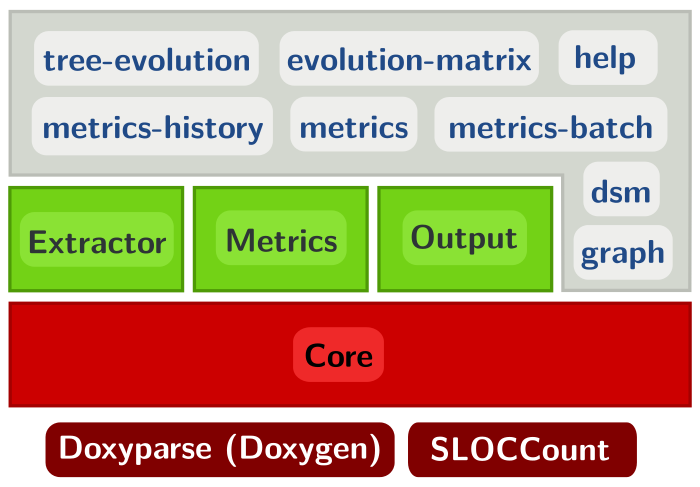
\includegraphics[scale=0.3]{imagens/analizo-architecture.png}
\caption{Arquitetura do Analizo, usando Layered Style \cite{Clements2002}}
\label{arquitetura-analizo}
\end{figure}

O {\it Core} contém as estruturas de dados usadas para armazenar informações a
respeito do código-fonte sendo analisado, como a lista de módulos\footnote{o
conceito ``módulo'' é usado como um termo abrangente para designar diferentes
tipos de estruturas usados em desenvolvimento de software, como classes e
arquivos fonte C}, elementos dentro de cada módulo (atributos, variáveis,
métodos, funções), informações de dependência (chamada, herança, etc). Esta
camada implementa a maior parte da lógica de negócio do Analizo, e não depende
de nenhuma outra camada.

A camada {\it Extractor} lida com as informaçoes de código-fonte obtidas pelas
diferentes estratégias implementadas no Analizo. Os extratores obtém
informações do código-fonte e armazenam em estruturas de dados da camada {\it
Core}. Adicionar um novo extrator requer apenas a criação de uma nova subclasse
que faça interface com uma ferramenta externa ou que ela própria realize análise
de código-fonte. Atualmente existem dois extratores, ambos fazem interface
com ferramentas externas de análise estática de código-fonte:

\begin{itemize}

  \item {\it Analizo::Extractor::Doxyparse} é uma interface para o Doxyparse,
  um parser de código-fonte para C, C++ e Java desenvolvida por nosso grupo de
  pesquisa\cite{Costa2009}. Doxyparse é baseado no
  Doxygen\footnote{doxygen.org}, um sistema de documentação multi-linguagem.

  \item {\it Analizo::Extractor::Sloccount} é uma interface para o
  Sloccount\footnote{dwheeler.com/sloccount} desenvolvido por David A. Wheeler,
  uma ferramenta que calcula o número efetivo de linhas de código.

\end{itemize}

As outras camadas intermediárias são {\it Metrics} e {\it Output}. A camada
{\it Metrics} processa as estruturas de dados do {\it Core} para calcular
métricas, até o momento Analizo suporta um conjunto razoável de métricas
(listadas na Seção \ref{metricas}), uma representação desta camada pode ser
vista no diagrama da Figura \ref{arquitetura-metrics-analizo}. A camada {\it
Output} é responsável por lidar com diferentes formatos de arquivos.
Atualmente, apenas o formato DOT é implementado no Analizo para representar
grafo de dependencia, adicionar novos formatos é simplesmente adicionar novas
classes nesta camada.

\begin{figure}[H]
\center
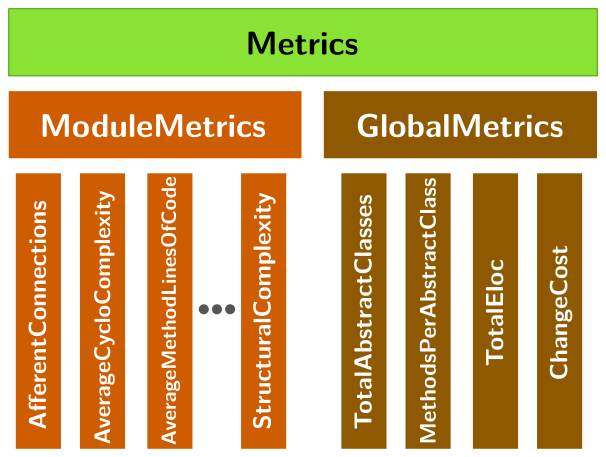
\includegraphics[scale=0.4]{imagens/analizo-metrics-architecture.png}
\caption{Arquitetura do módulo metrics em detalhe, usando Layered Style \cite{Clements2002}}
\label{arquitetura-metrics-analizo}
\end{figure}

A camada {\it Tools} fornece um conjunto de ferramentas de linha de comando que
constituem a interface do analizo, tanto para usuários finais quanto para
aplicações de mais alto nível. Estas ferramentas usam serviços providos pelas
outras camadas: eles instanciam as estruturas de dados do {\it Core},
inicializam um ou mais extratores, opcionalmente executam o processador de
métricas, instanciam um módulo de formato de saída, e gerencia todos eles para
prover o resultado desejado. A maioria das funcionalidades descritas na Seção
\ref{funcionalidades} são implementadas na camada {\it Tools} do Analizo.

Estas ferramentas são pensadas na filosofia UNIX: fazem uma tarefa
especializada e geram uma saída que pode ser utilizada como entrada para outras
ferramentas, seja para o próprio Analizo ou para ferramentas externas. Algumas das
ferramentas implementadas no Analizo são feitas consumindo saída gerada por
outra ferramenta ao invés de manipular explicitamente os internos do Analizo,
algumas outras são desenhadas para prover saída em formato específico para
aplicacoes externas, como por exemplo programas para desenho de grafos ou
visualização de dados.

\subsection{Funcionalidades}\label{funcionalidades}

\subsubsection{Análise de código-fonte multi-linguagem}

Atualmente Analizo suporta análise de código-fonte escrito em C, C++ e Java.
Entretanto, pode ser facilmente estendido para suportar outras linguagens pois
pode potencialmente suportar as inúmeras outras linguagens suportadas pelo Doxygen.

\subsubsection{Métricas}\label{metricas}

O Analizo suporta tanto métricas em nível de projeto, que é calculada para todo o projeto,
quanto métricas em nível de módulos, que é calculado individualmente para cada módulo.
No nível de projeto, Analizo também provê estatística descritiva básica para cada métrica em
nível de módulo: soma, média, mediana, moda, desvio padrão, variância, skewness e kurtosis da
distribuição, valores mínimo e maximo. As seguintes métricas são suportadas até o momento:

\begin{itemize}

  \item Métricas em nível de projeto: Change Cost, Total Abstract Classes,
  Total Coupling Factor, Total Effective Lines of Code, Total Lines of Code,
  Methods per Abstract Class, Total Number of Modules, Total number of modules
  with at least one defined attributes, Total number of modules with at least
  one defined method, Total Number of Methods.

  \item Métricas em nível de módulo: Afferent Connections per Class, Average
  Cyclomatic Complexity per Method, Average Method Lines of Code, Argument with
  'nonnull' attribute passed null, Average Number of Parameters per Method,
  Allocator sizeof operand mismatch, Assigned value is garbage or undefined,
  Bad deallocator, Bad free, Coupling Between Objects, Dead assignment,
  Divisions by zero, Double free, Depth of Inheritance Tree, Dereference of
  null pointer, Dereference of undefined pointer value, Potential buffer
  overflow in call to 'gets', Lack of Cohesion of Methods, Lines of Code,
  Memory leak, Max Method LOC, Number of Attributes, Number of Children, Number
  of Methods, Number of Public Attributes, Number of Public Methods,
  Out-of-bound array access, Offset free, Potential insecure temporary file in
  call 'mktemp', Response for a Class, Result of operation is garbage or
  undefined, Return of stack variable address, Stack address stored into global
  variable, Structural Complexity, Undefined allocation of 0 bytes,
  Use-after-free, Uninitialized argument value.

\end{itemize}

É possível especificar que certos diretórios dentro do projeto não devem ser
analisados, de forma que o Analizo ignore tais arquivos durante a análise e o
cálculo de métricas.

\subsubsection{Processamento em lote}\label{lote}

A maioria dos estudos quantitativos em Engenharia de Software envolve aquisição
de métricas de código-fonte de um grande número de projetos, processar cada
projeto individualmente é pouco prático, passível de erros e difícil de
repetir. Analizo pode processar multiplos projetos em lote e produzir arquivo
de dados CSV com métricas de cada projeto, bem como um resumo com as métricas
em nível de projeto de todos os projetos. Estes arquivos de dados podem ser
facilmente importados em ferramentas de estatística ou planilhas para análise
futura. Esta capacidade de processar em lote pode também ser utilizada para
analisar várias versões de um mesmo projeto, especialmente útil em estudos
sobre evolução de software.

Este processamento em lote pode se beneficiar de processamento paralelo dando
mais agilidade e na análise e reduzindo o tempo total de processamento.  A
saída pode ser também escrita diretamente em um banco de dados relacional ao
invés de gerar arquivos CSV. Outro recurso voltado à performance é um sistema
de cache para as informações previamente calculadas, evitando repetição de
processamento.

\subsubsection{Histórico de métricas}

Algumas vezes pesquisadores precisam processar o histórico de projetos de
software de uma forma mais escalável. Analizo pode processar repositórios de
controle de versão e prover arquivo de dados CSV com valores de métricas para
cada revisão onde o código-fonte foi alterado no projeto, ou pode também gravar
os valores diretamente num banco de dados ao invés de usar arquivos CSV. Repositórios Git e
Subversion são suportados diretamente, repositórios CVS devem ser convertidos
para Git de forma manual.

\subsubsection{Grafo de dependência}

Analizo pode gerar saída com informações sobre dependência entre as entidades
do projeto em um formato adequado para processamento por ferramentas de
renderização de grafos do Graphviz\footnote{graphviz.org}. A Figura
\ref{sample-graph} apresenta um exemplo de grafo desenhado pela ferramenta {\it
dot} do Graphviz a partir da saída gerada pelo Analizo {\it graph}.

\begin{figure}[h]
\center
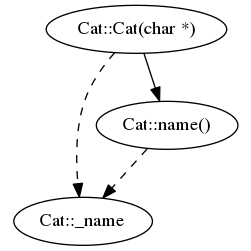
\includegraphics[scale=0.4]{imagens/sample-graph.png}
\caption{Exemplo de grafo de dependência}
\label{sample-graph}
\end{figure}

\subsubsection{Matriz de evolução}

Outra funcionalidade útil do Analizo é a visualização de matrizes de evolução
\cite{Lanza2001}. Ao processar cada release de um projeto (ver Seção
\ref{lote}), o usuário pode solicitar a criação de uma matrix de evolução a
partir de arquivos de dados individuais. A Figura \ref{sample-evolution-matrix}
apresenta um exemplo de uma matrix produzida pelo Analizo.

\begin{figure}[h]
\center
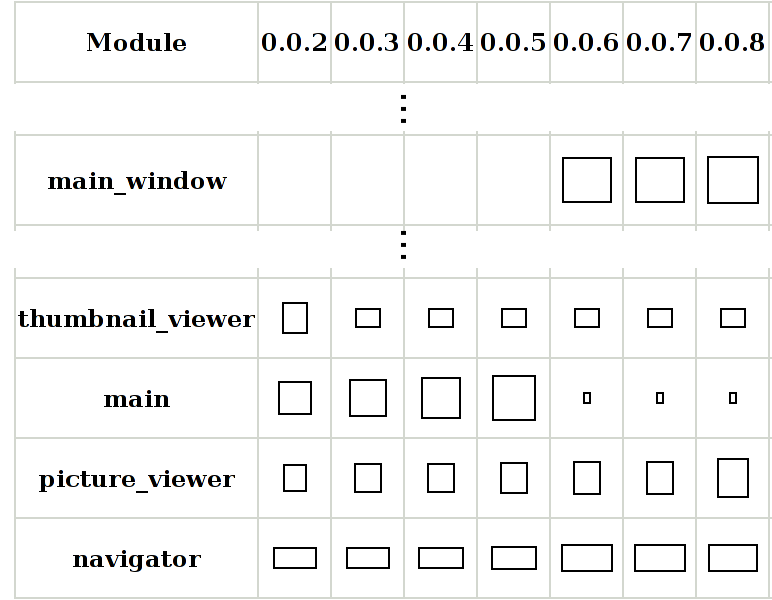
\includegraphics[scale=0.2]{imagens/sample-evolution-matrix.png}
\caption{Exemplo de matrix de evolução}
\label{sample-evolution-matrix}
\end{figure}

\subsubsection{Matriz de estrutura de projeto}

Uma funcionalidade recente do Analizo é a representação visual do
relacionamento entre os módulos do projeto em forma de uma Matriz de estrutura
de projeto ({\it Design Structure Matrix}) \cite{Maccormack2006}, uma DSM é a
representação de um grafo de dependência em forma de uma matriz quadrada. Um
exemplo gerado pelo Analizo pode ser visto na Figura \ref{sample-dsm}.

\begin{figure}[h]
\center
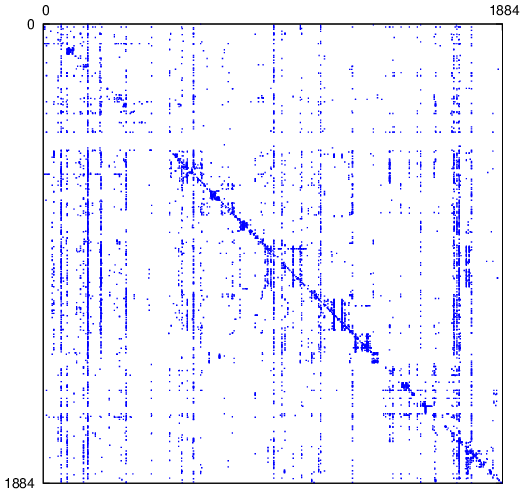
\includegraphics[scale=0.3]{imagens/sample-dsm.png}
\caption{Exemplo de matrix de estrutura de projeto}
\label{sample-dsm}
\end{figure}

\subsection{Uso em trabalhos de pesquisa}
\label{trabalhos-analizo}

Analizo tem sido extensivamente usada por nosso grupo de pesquisa em diversos
estudos:

\begin{itemize}

  \item \cite{Amaral2009} usou o grafo de dependencia gerado pelo Analizo para
  gerar uma matriz de evolução em um estudo de caso com o projeto VLC.

  \item \cite{Costa2009} fez uma comparação entre diferentes estratégias para
  extração de informação de dependencias entre módulos do código-fonte,
  resultando no desenvolvimento do Doxyparse - o extrator baseado no Doxygen do
  Analizo.

  \item \cite{Terceiro2009} usou métricas em um estudo exploratório sobre a
  evolução da complexidade estrutural em projetos de software livre escritos em
  C.

  \item \cite{Morais2009} usou a ferramenta de métricas do Analizo como backend
  para o Kalibro, um software para avaliação e observação de métricas de código-fonte.
  
  \item \cite{Terceiro2010} usou o processamento de histórico de métricas para
  realizar um estudo exploratório sobre a evolução da complexidade estrutural em
  7 projetos de servidor web de diferentes tamanhos.

  \item \cite{Meirelles2010} usou o processamento em lote do Analizo para
  processas o código-fonte de mais de 6000 projetos de software livre do
  repositório Sourceforge.net.

  \item \cite{Meirelles2011} usou o Analizo em um estudo sobre impacto de
  métricas de código-fonte na atratividade de projetos de softwares livres.

  \item \cite{Terceiro2012Understanding} usou o Analizo para investigar fatores
  que influenciam na evolução da complexidade estrutural em projetos de software
  livres.

  \item \cite{Silva2012} usou o Analizo para minerar 16000 revisões de
  repositórios de projetos de software para investigar o potencial de uma nova
  métrica chamada Lack of Concern-based Cohesion.

  \item \cite{Ronaldo2015} utilizou o Analizo para extrair métricas de
  código-fonte de 14 versões do sistema Android e estudar a evoluçao da API e
  seus aplicativos.

\end{itemize}

A maioria destes trabalhos contribuíram com melhorias para o Analizo, fazendo
dele ainda mais apropriado para pesquisas envolvendo análise de código-fonte.

\subsection{Considerações finais}

Apresentamos o Analizo, um conjunto de ferramentas para análise e
visualização de código-fonte com suporte a C, C++ e Java. Analizo é útil tanto
para pesquisadores trabalhando com análise de código-fonte quanto para
profissionais que precisam analisar seus projetos em busca de
potenciais problemas ou melhorias.

Analizo é software livre, licenciado sob a GNU General Public License versão 3.
Seu código-fonte, bem como pacotes binários, manuais e tutoriais podem ser
obtidos em http://analizo.org. Todas as ferramentas são auto-documentadas e
podem ser consultadas como páginas de manual UNIX. Analizo é escrito em Perl.


%------------------------------------------%

\xchapter{Conclusões}
{}
\label{conclusoes}

(pendente)

Trabalhos futuros:

usar mais dimensões na caracterização, ver issue #18

usar caracterizacao ja realizadas em outros trabalhor, ver issue #22


%------------------------------------------%

\backmatter
\bibliography{bibliografia}

\appendix

%------------------------------------------%

% \xchapter{Análise exploratória dos valores das métricas}
{Este capítulo apresenta uma análise exploratória e interpretação dos valores das métricas coletadas para cada ferramenta.}
\label{analise-metricas}

\subsection{Conexões aferentes de uma classe (ACC)}

ACC é um valor parcial de uma das métricas MOOD (Metrics for Object Oriented
Design) \cite{Brito1994} e mede o nível de acoplamento de uma classe. O
cálculo é feito através do número de classes que fazem referência a um outra
por meio de métodos ou atributos.

As Tabelas \ref{metrica-acc} e \ref{metrica-acc-industria} apresentam os
valores da métrica ACC para as ferramentas da academia e da indústria,
respectivamente.

%% begin.rcode metrica-acc, fig.align='center', results="asis"
% table = percentis_by_project("acc")
% total_modules = metric_by_project("total_modules")
% table = add_column(table, total_modules, colname = "classes")
% knitr_latex_table(table, "percentis da métrica ACC para as ferramentas da academia", "metrica-acc")
%% end.rcode

Duas ferramentas, accessanalysis e error-prone, tiveram valor 0 no percentil
75, é estranho que 75\% das classes destas 2 ferramentas, ambas escritas em
Java, não façam acesso através de métodos ou atributos a nenhuma outra classe
do mesmo sistema.

%% begin.rcode metrica-acc-industria, fig.align='center', results="asis"
% table = percentis_by_nist_project("acc")
% total_modules = metric_by_nist_project("total_modules")
% table = add_column(table, total_modules, colname = "classes")
% knitr_latex_table(table, "percentis da métrica ACC para as ferramentas da indústria", "metrica-acc-industria")
%% end.rcode

As ferramentas cqual e uno tiveram valores no percentil 75\% bem acima das
demais ferramentas, 24 e 34, respectivamente. Onde entre todas as outras o
maior valor foi 8.

\subsection{Média de complexidade ciclomática por método (ACCM)}

ACCM contabiliza o número de caminhos independentes que métodos de uma classe
pode seguir em sua execução. O cálculo é feito a partir do número de
estruturas condicionais encontrados nos métodos de um programa.

As Tabelas \ref{metrica-accm} e \ref{metrica-accm-industria} apresentam os
valores da métrica ACCM para as ferramentas da academia e da indústria,
respectivamente.

%% begin.rcode metrica-accm, fig.align='center', results="asis"
% table = percentis_by_project("accm")
% total_modules = metric_by_project("total_modules")
% table = add_column(table, total_modules, colname = "classes")
% knitr_latex_table(table, "percentis da métrica ACCM para as ferramentas da academia", "metrica-accm")
%% end.rcode

Esta métrica apresenta um comportamento sem muitas exceções dentro de cada
percentil, com intervalos entre 1.0 e 2.1 para percentil 75\%, 2.0 e 3.4 para
percentil 90\% e 2.9 e 5.0 para percentil 95\%.

%% begin.rcode metrica-accm-industria, fig.align='center', results="asis"
% table = percentis_by_nist_project("accm")
% total_modules = metric_by_nist_project("total_modules")
% table = add_column(table, total_modules, colname = "classes")
% knitr_latex_table(table, "percentis da métrica ACCM para as ferramentas da indústria", "metrica-accm-industria")
%% end.rcode

Também entre as ferramentas da indústria esta métrica não apresenta variações
muito grandes, com intervalos entre 1.0 e 6.9 para 75\%, 2.0 e 8.9 para
percentil 90\% e entre 4.0 e 15.6 para 95\%.

\subsection{Média do número de linhas de código por método (AMLOC)}

AMLOC é a média do número de linhas dos métodos de um módulo, apenas linhas
com código executável é calculada, comentários e linhas em branco são
desconsideradas do cálculo.

As Tabelas \ref{metrica-amloc} e \ref{metrica-amloc-industria} apresentam a
métrica AMLOC para as ferramentas da academia e da indústria, respectivamente.

%% begin.rcode metrica-amloc, fig.align='center', results="asis"
% table = percentis_by_project("amloc")
% total_modules = metric_by_project("total_modules")
% table = add_column(table, total_modules, colname = "classes")
% knitr_latex_table(table, "percentis da métrica AMLOC para as ferramentas da academia", "metrica-amloc")
%% end.rcode

Os valores para ferramentas da academia não nos chama atenção para nada
especial, com intervalos entre 5.4 e 14.5 para o percentil 75\%, entre 10.7 e
31.5 pra percentil 90\% e entre 15.4 e 51.4 para 95\%.

%% begin.rcode metrica-amloc-industria, fig.align='center', results="asis"
% table = percentis_by_nist_project("amloc")
% total_modules = metric_by_nist_project("total_modules")
% table = add_column(table, total_modules, colname = "classes")
% knitr_latex_table(table, "percentis da métrica AMLOC para as ferramentas da indústria", "metrica-amloc-industria")
%% end.rcode

Para a indústria os intervalos foram entre 7.0 e 36.9 para o percentil 75\%,
entre 16.0 e 62.1 para percentil 90\% e entre 22.0 e 119.7 para 95\%. A
ferramenta chama atenção por apresentr o menor valor no percentil 75\%, 7, e o
maior valor no prcentil 95\%, 119.7.

\subsection{Média do número de parâmetros por método (ANPM)}

ANPM é a média de parâmetros dos métodos de uma classe.

As Tabelas \ref{metrica-anpm} e \ref{metrica-anpm-industria} apresentam a
métrica ANPM para as ferramentas da academia e da indústria, respectivamente.

%% begin.rcode metrica-anpm, fig.align='center', results="asis"
% table = percentis_by_project("anpm")
% total_modules = metric_by_project("total_modules")
% table = add_column(table, total_modules, colname = "classes")
% knitr_latex_table(table, "percentis da métrica ANPM para as ferramentas da academia", "metrica-anpm")
%% end.rcode

%% begin.rcode metrica-anpm-industria, fig.align='center', results="asis"
% table = percentis_by_nist_project("anpm")
% total_modules = metric_by_nist_project("total_modules")
% table = add_column(table, total_modules, colname = "classes")
% knitr_latex_table(table, "percentis da métrica ANPM para as ferramentas da indústria", "metrica-anpm-industria")
%% end.rcode

\subsection{Acoplamento entre objetos (CBO)}

CBO é a recíproca da métrica ACC e mede quantas classes são utilizadas por uma
certa classe.

As Tabelas \ref{metrica-cbo} e \ref{metrica-cbo-industria} apresentam a
métrica CBO para as ferramentas da academia e da indústria, respectivamente.

%% begin.rcode metrica-cbo, fig.align='center', results="asis"
% table = percentis_by_project("cbo")
% total_modules = metric_by_project("total_modules")
% table = add_column(table, total_modules, colname = "classes")
% knitr_latex_table(table, "percentis da métrica CBO para as ferramentas da academia", "metrica-cbo")
%% end.rcode

%% begin.rcode metrica-cbo-industria, fig.align='center', results="asis"
% table = percentis_by_nist_project("cbo")
% total_modules = metric_by_nist_project("total_modules")
% table = add_column(table, total_modules, colname = "classes")
% knitr_latex_table(table, "percentis da métrica CBO para as ferramentas da indústria", "metrica-cbo-industria")
%% end.rcode

\subsection{Profundidade da árvore de herança (DIT)}

DIT mede a profundidade que uma classe se encontra na árvore de herança.

Os intervalos sugeridos são: até 2 (bom); entre 2 e 4 (regular); de 4 em
diante (ruim).

As Tabelas \ref{metrica-dit} e \ref{metrica-dit-industria} apresentam a
métrica DIT para as ferramentas da academia e da indústria, respectivamente.

%% begin.rcode metrica-dit, fig.align='center', results="asis"
% table = percentis_by_project("dit")
% total_modules = metric_by_project("total_modules")
% table = add_column(table, total_modules, colname = "classes")
% knitr_latex_table(table, "percentis da métrica DIT para as ferramentas da academia", "metrica-dit")
%% end.rcode

%% begin.rcode metrica-dit-industria, fig.align='center', results="asis"
% table = percentis_by_nist_project("dit")
% total_modules = metric_by_nist_project("total_modules")
% table = add_column(table, total_modules, colname = "classes")
% knitr_latex_table(table, "percentis da métrica DIT para as ferramentas da indústria", "metrica-dit-industria")
%% end.rcode

\subsection{Ausência de coesão em métodos (LCOM4)}

LCOM4 calcula quantos conjuntos de métodos relacionados existem dentro de uma
classe, isto é, métodos que compartilham utilização de algum atributo ou que
se referenciam.

Os intervalos sugeridos para código C++ e Java são: até 2 (bom); entre 2 e 5
(regular); de 5 em diante (ruim).

As Tabelas \ref{metrica-lcom4} e \ref{metrica-lcom4-industria} apresentam a
métrica LCOM4 para as ferramentas da academia e da indústria, respectivamente.

%% begin.rcode metrica-lcom4, fig.align='center', results="asis"
% table = percentis_by_project("lcom4")
% total_modules = metric_by_project("total_modules")
% table = add_column(table, total_modules, colname = "classes")
% knitr_latex_table(table, "percentis da métrica LCOM4 para as ferramentas da academia", "metrica-lcom4")
%% end.rcode

%% begin.rcode metrica-lcom4-industria, fig.align='center', results="asis"
% table = percentis_by_nist_project("lcom4")
% total_modules = metric_by_nist_project("total_modules")
% table = add_column(table, total_modules, colname = "classes")
% knitr_latex_table(table, "percentis da métrica LCOM4 para as ferramentas da indústria", "metrica-lcom4-industria")
%% end.rcode

\subsection{Número de linhas de código (LOC)}

LOC é a medida mais comum para o tamanho de um software, conta o número linhas
executáveis excluindo linhas em branco e comentários.

Os intervalos sugeridos para o LOC de uma classe (Java e C++) são: até 70
(bom); entre 70 e 130 (regular); de 130 em diante (ruim).

As Tabelas \ref{metrica-loc} e \ref{metrica-loc-industria} apresentam a
métrica LOC para as ferramentas da academia e da indústria, respectivamente.

%% begin.rcode metrica-loc, fig.align='center', results="asis"
% table = percentis_by_project("loc")
% total_modules = metric_by_project("total_modules")
% table = add_column(table, total_modules, colname = "classes")
% knitr_latex_table(table, "percentis da métrica LOC para as ferramentas da academia", "metrica-loc")
%% end.rcode

%% begin.rcode metrica-loc-industria, fig.align='center', results="asis"
% table = percentis_by_nist_project("loc")
% total_modules = metric_by_nist_project("total_modules")
% table = add_column(table, total_modules, colname = "classes")
% knitr_latex_table(table, "percentis da métrica LOC para as ferramentas da indústria", "metrica-loc-industria")
%% end.rcode

\subsection{Número de atributos (NOA)}

NOA contabiliza o número de atributos de uma classe.

As Tabelas \ref{metrica-noa} e \ref{metrica-noa-industria} apresentam a
métrica NOA para as ferramentas da academia e da indústria, respectivamente.

%% begin.rcode metrica-noa, fig.align='center', results="asis"
% table = percentis_by_project("noa")
% total_modules = metric_by_project("total_modules")
% table = add_column(table, total_modules, colname = "classes")
% knitr_latex_table(table, "percentis da métrica NOA para as ferramentas da academia", "metrica-noa")
%% end.rcode

%% begin.rcode metrica-noa-industria, fig.align='center', results="asis"
% table = percentis_by_nist_project("noa")
% total_modules = metric_by_nist_project("total_modules")
% table = add_column(table, total_modules, colname = "classes")
% knitr_latex_table(table, "percentis da métrica NOA para as ferramentas da indústria", "metrica-noa-industria")
%% end.rcode

\subsection{Número de filhos (NOC)}

NOC é o número total de flhos de uma classe.

As Tabelas \ref{metrica-noc} e \ref{metrica-noc-industria} apresentam a
métrica NOC para as ferramentas da academia e da indústria, respectivamente.

%% begin.rcode metrica-noc, fig.align='center', results="asis"
% table = percentis_by_project("noc")
% total_modules = metric_by_project("total_modules")
% table = add_column(table, total_modules, colname = "classes")
% knitr_latex_table(table, "percentis da métrica NOC para as ferramentas da academia", "metrica-noc")
%% end.rcode

%% begin.rcode metrica-noc-industria, fig.align='center', results="asis"
% table = percentis_by_nist_project("noc")
% total_modules = metric_by_nist_project("total_modules")
% table = add_column(table, total_modules, colname = "classes")
% knitr_latex_table(table, "percentis da métrica NOC para as ferramentas da indústria", "metrica-noc-industria")
%% end.rcode

\subsection{Número de métodos (NOM)}

NOM indica o tamanho das classes em termos das suas operações implementadas.

As Tabelas \ref{metrica-nom} e \ref{metrica-nom-industria} apresentam a
métrica NOM para as ferramentas da academia e da indústria, respectivamente.

%% begin.rcode metrica-nom, fig.align='center', results="asis"
% table = percentis_by_project("nom")
% total_modules = metric_by_project("total_modules")
% table = add_column(table, total_modules, colname = "classes")
% knitr_latex_table(table, "percentis da métrica NOM para as ferramentas da academia", "metrica-nom")
%% end.rcode

%% begin.rcode metrica-nom-industria, fig.align='center', results="asis"
% table = percentis_by_nist_project("nom")
% total_modules = metric_by_nist_project("total_modules")
% table = add_column(table, total_modules, colname = "classes")
% knitr_latex_table(table, "percentis da métrica NOM para as ferramentas da indústria", "metrica-nom-industria")
%% end.rcode

\subsection{Número de atributos públicos (NPA)}

NPA mede o encapsulamento entre classes.

Os intervalos sugeridos para Java e C++ são: até 1 (bom); entre 1 e 9
(regular); de 9 em diante (ruim).

As Tabelas \ref{metrica-npa} e \ref{metrica-npa-industria} apresentam a
métrica NPA para as ferramentas da academia e da indústria, respectivamente.

%% begin.rcode metrica-npa, fig.align='center', results="asis"
% table = percentis_by_project("npa")
% total_modules = metric_by_project("total_modules")
% table = add_column(table, total_modules, colname = "classes")
% knitr_latex_table(table, "percentis da métrica NPA para as ferramentas da academia", "metrica-npa")
%% end.rcode

%% begin.rcode metrica-npa-industria, fig.align='center', results="asis"
% table = percentis_by_nist_project("npa")
% total_modules = metric_by_nist_project("total_modules")
% table = add_column(table, total_modules, colname = "classes")
% knitr_latex_table(table, "percentis da métrica NPA para as ferramentas da indústria", "metrica-npa-industria")
%% end.rcode

\subsection{Número de métodos públicos (NPM)}

NPM indica o tamanho da ``interface'' da classe.

Os intervalos sugeridos para Java e C++ são: até 10 (bom); entre 10 e 40
(regular); de 40 em diante (ruim).

As Tabelas \ref{metrica-npm} e \ref{metrica-npm-industria} apresentam a
métrica NPA para as ferramentas da academia e da indústria, respectivamente.

%% begin.rcode metrica-npm, fig.align='center', results="asis"
% table = percentis_by_project("npm")
% total_modules = metric_by_project("total_modules")
% table = add_column(table, total_modules, colname = "classes")
% knitr_latex_table(table, "percentis da métrica NPM para as ferramentas da academia", "metrica-npm")
%% end.rcode

%% begin.rcode metrica-npm-industria, fig.align='center', results="asis"
% table = percentis_by_nist_project("npm")
% total_modules = metric_by_nist_project("total_modules")
% table = add_column(table, total_modules, colname = "classes")
% knitr_latex_table(table, "percentis da métrica NPM para as ferramentas da indústria", "metrica-npm-industria")
%% end.rcode

\subsection{Resposta para uma classe (RFC)}

RFC conta o número de métodos que podem ser executados a partir de uma
mensagem enviada a um objeto dessa classe.

As Tabelas \ref{metrica-rfc} e \ref{metrica-rfc-industria} apresentam a
métrica RFC para as ferramentas da academia e da indústria, respectivamente.

%% begin.rcode metrica-rfc, fig.align='center', results="asis"
% table = percentis_by_project("rfc")
% total_modules = metric_by_project("total_modules")
% table = add_column(table, total_modules, colname = "classes")
% knitr_latex_table(table, "percentis da métrica RFC para as ferramentas da academia", "metrica-rfc")
%% end.rcode

%% begin.rcode metrica-rfc-industria, fig.align='center', results="asis"
% table = percentis_by_nist_project("rfc")
% total_modules = metric_by_nist_project("total_modules")
% table = add_column(table, total_modules, colname = "classes")
% knitr_latex_table(table, "percentis da métrica RFC para as ferramentas da indústria", "metrica-rfc-industria")
%% end.rcode

\subsection{Complexidade estrutural (SC)}

SC é medida através da combinação das métricas de acoplamento (CBO) e coesão
(LCOM4).

As Tabelas \ref{metrica-sc} e \ref{metrica-sc-industria} apresentam a
métrica SC para as ferramentas da academia e da indústria, respectivamente.

%% begin.rcode metrica-sc, fig.align='center', results="asis"
% table = percentis_by_project("sc")
% total_modules = metric_by_project("total_modules")
% table = add_column(table, total_modules, colname = "classes")
% knitr_latex_table(table, "percentis da métrica SC para as ferramentas da academia", "metrica-sc")
%% end.rcode

%% begin.rcode sumario-sc, fig.align='center', results="asis"
% table = percentis_by_project("sc")
% table = table[-1:-5,]
% table = table[-4,]
% xt = xtable(summary(t(table)), caption="resumo da métrica SC nos percentis 75, 90 e 95 para as ferramentas da academia")
% print(xt, table.placement="H", caption.placement="top")
%% end.rcode

%% begin.rcode metrica-sc-industria, fig.align='center', results="asis"
% table = percentis_by_nist_project("sc")
% total_modules = metric_by_nist_project("total_modules")
% table = add_column(table, total_modules, colname = "classes")
% knitr_latex_table(table, "percentis da métrica SC para as ferramentas da indústria", "metrica-sc-industria")
%% end.rcode

%% begin.rcode sumario-sc-industria, fig.align='center', results="asis"
% table = percentis_by_nist_project("sc")
% table = table[-1:-5,]
% table = table[-4,]
% xt = xtable(summary(t(table)), caption="resumo da métrica SC nos percentis 75, 90 e 95 para as ferramentas da indústria")
% print(xt, table.placement="H", caption.placement="top")
%% end.rcode

\xchapter{Histogramas}{}

%% begin.rcode histograma-acc, fig.align='center', results="asis"
% histograma('acc', 'histograma da métrica ACC para todas as ferramentas')
%% end.rcode

%% begin.rcode histograma-accm, fig.align='center', results="asis"
% histograma('accm', 'histograma da métrica ACCM para todas as ferramentas')
%% end.rcode

%% begin.rcode histograma-cbo, fig.align='center', results="asis"
% histograma('cbo', 'histograma da métrica CBO para todas as ferramentas')
%% end.rcode

%% begin.rcode histograma-loc, fig.align='center', results="asis"
% histograma('loc', 'histograma da métrica LOC para todas as ferramentas')
%% end.rcode

%% begin.rcode histograma-amloc, fig.align='center', results="asis"
% histograma('amloc', 'histograma da métrica AMLOC para todas as ferramentas')
%% end.rcode

%% begin.rcode histograma-anpm, fig.align='center', results="asis"
% histograma('anpm', 'histograma da métrica ANPM para todas as ferramentas')
%% end.rcode

%% begin.rcode histograma-dit, fig.align='center', results="asis"
% histograma('dit', 'histograma da métrica DIR para todas as ferramentas')
%% end.rcode

%% begin.rcode histograma-rfc, fig.align='center', results="asis"
% histograma('rfc', 'histograma da métrica RFC para todas as ferramentas')
%% end.rcode

%% begin.rcode histograma-noa, fig.align='center', results="asis"
% histograma('noa', 'histograma da métrica NOA para todas as ferramentas')
%% end.rcode

%% begin.rcode histograma-noc, fig.align='center', results="asis"
% histograma('noc', 'histograma da métrica NOC para todas as ferramentas')
%% end.rcode

%% begin.rcode histograma-npm, fig.align='center', results="asis"
% histograma('npm', 'histograma da métrica NPM para todas as ferramentas')
%% end.rcode

%% begin.rcode histograma-nom, fig.align='center', results="asis"
% histograma('nom', 'histograma da métrica NOM para todas as ferramentas')
%% end.rcode

%% begin.rcode histograma-sc, fig.align='center', results="asis"
% histograma('sc', 'histograma da métrica SC para todas as ferramentas')
%% end.rcode



%------------------------------------------%

\xchapter{Edições das conferências revisadas}
{Este capítulo apresenta as edições das conferências incluídas na revisão
estruturada.}
\label{edicoes-conferencias}

\section{SCAM - Source Code Analysis and Manipulation Working Conference}

\begin{itemize}
  \item SCAM 2001 - {\small http://ieeexplore.ieee.org/xpl/mostRecentIssue.jsp?punumber=7667}
  \item SCAM 2002 - {\small http://ieeexplore.ieee.org/xpl/mostRecentIssue.jsp?punumber=6494367}
  \item SCAM 2003 - {\small http://ieeexplore.ieee.org/xpl/mostRecentIssue.jsp?punumber=8773}
  \item SCAM 2004 - {\small http://ieeexplore.ieee.org/xpl/mostRecentIssue.jsp?punumber=9523}
  \item SCAM 2005 - {\small http://ieeexplore.ieee.org/xpl/mostRecentIssue.jsp?punumber=10344}
  \item SCAM 2006 - {\small http://ieeexplore.ieee.org/xpl/mostRecentIssue.jsp?punumber=4026839}
  \item SCAM 2007 - {\small http://ieeexplore.ieee.org/xpl/mostRecentIssue.jsp?punumber=4362882}
  \item SCAM 2008 - {\small http://ieeexplore.ieee.org/xpl/mostRecentIssue.jsp?punumber=4637522}
  \item SCAM 2009 - {\small http://ieeexplore.ieee.org/xpl/mostRecentIssue.jsp?punumber=5279860}
  \item SCAM 2010 - {\small http://ieeexplore.ieee.org/xpl/mostRecentIssue.jsp?punumber=5600365}
  \item SCAM 2011 - {\small http://ieeexplore.ieee.org/xpl/mostRecentIssue.jsp?punumber=6063701}
  \item SCAM 2012 - {\small http://ieeexplore.ieee.org/xpl/mostRecentIssue.jsp?punumber=6389882}
  \item SCAM 2013 - {\small http://ieeexplore.ieee.org/xpl/mostRecentIssue.jsp?punumber=6636284}
  \item SCAM 2014 - {\small http://ieeexplore.ieee.org/xpl/mostRecentIssue.jsp?punumber=6970367}
  \item SCAM 2015 - {\small http://ieeexplore.ieee.org/xpl/mostRecentIssue.jsp?punumber=7321933}
\end{itemize}

\section{ASE - Automated Software Engineering}

Até o ano de 1996 a conferencia ASE se chamava KBSE - Knowledge-Based Software
Engineering Conference e a partir de 1997 passou a se chamar ASE - Automated
Software Conference.

\begin{itemize}
  \item ASE/KBSE 1991 - {\small http://ieeexplore.ieee.org/xpl/mostRecentIssue.jsp?punumber=5069}
  \item ASE/KBSE 1992 - {\small http://ieeexplore.ieee.org/xpl/mostRecentIssue.jsp?punumber=421}
  \item ASE/KBSE 1993 - {\small http://ieeexplore.ieee.org/xpl/mostRecentIssue.jsp?punumber=921}
  \item ASE/KBSE 1994 - {\small http://ieeexplore.ieee.org/xpl/mostRecentIssue.jsp?punumber=995}
  \item ASE/KBSE 1995 - {\small http://ieeexplore.ieee.org/xpl/mostRecentIssue.jsp?punumber=3518}
  \item ASE/KBSE 1996 - {\small http://ieeexplore.ieee.org/xpl/mostRecentIssue.jsp?punumber=4065}
  \item ASE 1997 - {\small http://ieeexplore.ieee.org/xpl/mostRecentIssue.jsp?punumber=5003}
  \item ASE 1998 - {\small http://ieeexplore.ieee.org/xpl/mostRecentIssue.jsp?punumber=5935}
  \item ASE 1999 - {\small http://ieeexplore.ieee.org/xpl/mostRecentIssue.jsp?punumber=6516}
  \item ASE 2000 - {\small http://ieeexplore.ieee.org/xpl/mostRecentIssue.jsp?punumber=7013}
  \item ASE 2001 - {\small http://ieeexplore.ieee.org/xpl/mostRecentIssue.jsp?punumber=7763}
  \item ASE 2002 - {\small http://ieeexplore.ieee.org/xpl/mostRecentIssue.jsp?punumber=8183}
  \item ASE 2003 - {\small http://ieeexplore.ieee.org/xpl/conhome.jsp?punumber=1000064}
  \item ASE 2004 - {\small http://ieeexplore.ieee.org/xpl/mostRecentIssue.jsp?punumber=9305}
  \item ASE 2005 - {\small http://dl.acm.org/citation.cfm?id=1101908}
  \item ASE 2006 - {\small http://ieeexplore.ieee.org/xpl/mostRecentIssue.jsp?punumber=4019543}
  \item ASE 2007 - {\small http://dl.acm.org/citation.cfm?id=1321631}
  \item ASE 2008 - {\small http://ieeexplore.ieee.org/xpl/mostRecentIssue.jsp?punumber=4639292}
  \item ASE 2009 - {\small http://ieeexplore.ieee.org/xpl/mostRecentIssue.jsp?punumber=5431684}
  \item ASE 2010 - {\small http://dl.acm.org/citation.cfm?id=1858996}
  \item ASE 2011 - {\small http://ieeexplore.ieee.org/xpl/mostRecentIssue.jsp?punumber=6093623}
  \item ASE 2012 - {\small http://ieeexplore.ieee.org/xpl/mostRecentIssue.jsp?punumber=6494367}
  \item ASE 2013 - {\small http://ieeexplore.ieee.org/xpl/mostRecentIssue.jsp?punumber=6684409}
  \item ASE 2014 - {\small http://dl.acm.org/citation.cfm?id=2642937}
  \item ASE 2015 - {\small http://ieeexplore.ieee.org/xpl/mostRecentIssue.jsp?punumber=7371449}
\end{itemize}


%------------------------------------------%

\end{document}

% vim: filetype=tex
